%%%%%%%%%%%%%%%%%%%%%%%%%%%%%%%%%%%%%%%%%
% Masters/Doctoral Thesis 
% LaTeX Template
% Version 1.43 (17/5/14)
%
% This template has been downloaded from:
% http://www.LaTeXTemplates.com
%
% Original authors:
% Steven Gunn 
% http://users.ecs.soton.ac.uk/srg/softwaretools/document/templates/
% and
% Sunil Patel
% http://www.sunilpatel.co.uk/thesis-template/
%
% License:
% CC BY-NC-SA 3.0 (http://creativecommons.org/licenses/by-nc-sa/3.0/)
%
% Note:
% Make sure to edit document variables in the Thesis.cls file
%
%%%%%%%%%%%%%%%%%%%%%%%%%%%%%%%%%%%%%%%%%

%----------------------------------------------------------------------------------------
%	PACKAGES AND OTHER DOCUMENT CONFIGURATIONS
%----------------------------------------------------------------------------------------

\documentclass[11pt, oneside]{Thesis} % The default font size and one-sided printing (no margin offsets)

\graphicspath{{../graphics/}} % Specifies the directory where pictures are stored

\usepackage[square, numbers, comma, sort&compress]{natbib} % Use the natbib reference package - read up on this to edit the reference style; if you want text (e.g. Smith et al., 2012) for the in-text references (instead of numbers), remove 'numbers' 

%from my usual papers
\usepackage{amsmath}
\usepackage{amssymb}
\usepackage{amsthm}
\usepackage{amscd}
\usepackage{amsfonts}
\usepackage{graphicx}%
%\usepackage{fancyhdr}
\usepackage{xcolor}
%\usepackage{cite}
\usepackage{physics}
\usepackage{float}
\usepackage{caption}
\usepackage{subcaption}
\usepackage{colortbl}

\usepackage{pdfpages}

%define some colors
\definecolor{Gray3}{gray}{0.6}
\definecolor{Gray6}{gray}{0.9}

\hypersetup{urlcolor=black, colorlinks=true} % Colors hyperlinks in blue - change to black if annoying
\title{\ttitle} % Defines the thesis title - don't touch this

\begin{document}

\frontmatter % Use roman page numbering style (i, ii, iii, iv...) for the pre-content pages

\setstretch{1.3} % Line spacing of 1.3

% Define the page headers using the FancyHdr package and set up for one-sided printing
\fancyhead{} % Clears all page headers and footers
\rhead{\thepage} % Sets the right side header to show the page number
\lhead{} % Clears the left side page header

\pagestyle{fancy} % Finally, use the "fancy" page style to implement the FancyHdr headers

\newcommand{\HRule}{\rule{\linewidth}{0.5mm}} % New command to make the lines in the title page

%code handling
\newcommand{\raven}{\texttt{RAVEN}}
\newcommand{\bison}{\texttt{BISON}}
\newcommand{\moose}{\texttt{MOOSE}}
\newcommand{\mammoth}{\texttt{MAMMOTH}}
\newcommand{\rattlesnake}{\texttt{RATTLESNAKE}}

% some handy math stuff
\newcommand{\expv}[1]{\ensuremath{\mathbb{E}[ #1]}}
\newcommand{\xs}[2]{\ensuremath{\Sigma_{#1}^{(#2)}}}
\newcommand{\intz}{\ensuremath{\int\limits_0^1}}
\newcommand{\intf}{\ensuremath{\int\limits_{-\infty}^\infty}}
\newcommand{\intzf}{\ensuremath{\int\limits_{0}^\infty}}
\newcommand{\LargerCdot}{\raisebox{-0.25ex}{\scalebox{1.2}{$\cdot$}}}
\newcommand{\hold}[1]{\ensuremath{\Big|_{#1}}}
\newcommand{\barhat}[1]{\hat{\bar{{#1}}}}
\newcommand{\intom}{\ensuremath{\int\limits_{\Omega}}}
\newcommand{\intomn}{\ensuremath{\int\limits_{\Omega_n}}}
\newcommand{\intomx}[1]{\ensuremath{\int\limits_{\Omega_{#1}}}}
\newcommand{\mlsum}[2]{\ensuremath{\sum_{\tiny\begin{array}{c}#1\end{array}}^{#2}}}
\newcommand{\mlprod}[2]{\ensuremath{\prod_{\tiny\begin{array}{c}#1\end{array}}^{#2}}}

\renewcommand{\vec}[1]{\mathbf{#1}}

% PDF meta-data
\hypersetup{pdftitle={\ttitle}}
\hypersetup{pdfsubject=\subjectname}
\hypersetup{pdfauthor=\authornames}
\hypersetup{pdfkeywords=\keywordnames}

%----------------------------------------------------------------------------------------
%	DECLARATION PAGE
%	Your institution may give you a different text to place here
%----------------------------------------------------------------------------------------
\clearpage

\includepdf[offset=75 -75,angle=0,pagecommand={}]{university/diss_approval_pdf}  
\clearpage % Start a new page
%----------------------------------------------------------------------------------------
%	TITLE PAGE
%----------------------------------------------------------------------------------------

\begin{titlepage}
\begin{center}

%\textsc{\LARGE \univname}\\[1.5cm] % University name
%\textsc{\Large Doctoral Thesis}\\[0.5cm] % Thesis type

%\HRule \\[0.4cm] % Horizontal line
{\huge \bfseries \ttitle}\\[0.4cm] % Thesis title
%\HRule \\[1.5cm] % Horizontal line
 
%\begin{minipage}{0.4\textwidth}
%\begin{flushleft}
  %\centering{
  \large
  by\\[1cm]
%\href{http://www.johnsmith.com}
  \authornames\\[1cm]% Author name - remove the \href bracket to remove the link
\normalsize
B.S., Physics, Brigham Young University-Idaho, 2010 \\
M.S., Nuclear Engineering, Oregon State University, 2013%}
%\end{minipage}
%\begin{minipage}{0.4\textwidth}
%\begin{flushright} \large
%\emph{Supervisor:} \\
%\href{http://www.jamessmith.com}
%{\supname} % Supervisor name - remove the \href bracket to remove the link  
%\end{flushright}
%\end{minipage}
\\[3cm]
\large DISSERTATION
\\[3cm]
 
\large \textit{Submitted in partial fulfillment of the requirements\\ 
for the degree of Doctor of Philosophy in}\\[0.3cm] % University requirement text
%\textit{in the}\\[0.4cm]
Nuclear Engineering
%\deptname
\\[1cm] % Research group name and department name
The University of New Mexico\\
Albuquerque, New Mexico
\\[2cm]
{\large December 2016}\\[4cm] % Date
%\includegraphics{Logo} % University/department logo - uncomment to place it
 
\vfill
\end{center}
\end{titlepage}

\clearpage % Start a new page
%%----------------------------------------------------------------------------------------
%%	DEDICATION
%%----------------------------------------------------------------------------------------
%
\setstretch{1.3} % Return the line spacing back to 1.3
%
%\pagestyle{empty} % Page style needs to be empty for this page
%
\setcounter{page}{3}
\begin{center}
\dedicatory{To my dear wife, Heather, whose support has provided refuge and 
sanctuary through my every endeavor, and to my children, who remind me who I am.} % Dedication text
\end{center}
%
\addtocontents{toc}{\vspace{2em}} % Add a gap in the Contents, for aesthetics

%----------------------------------------------------------------------------------------
%	ACKNOWLEDGEMENTS
%----------------------------------------------------------------------------------------

\setstretch{1.3} % Reset the line-spacing to 1.3 for body text (if it has changed)
%
\acknowledgements{\addtocontents{toc}{\vspace{1em}} % Add a gap in the Contents, for aesthetics
%
\begin{em}
\vfill
First and foremost, I offer my thanks to my adviser, Dr. Anil Prinja, for his dedicated support of my research and
my family as we've explored this work.  Without him, this opportunity would not have been possible.

\vfill
On a similar note, I extend warm thanks to the \raven{} team: Drs. Cristian Rabiti, Andrea Alfonsi, 
Joshua Cogliati, Diego Mandelli, Bob Kinoshita, CongJian Wang, and Dan
Maljovec.  These remarkable gentlemen have provided no end of assistance as I learned, used, and contributed
to their (or should I say ``our'') project.  It has been an honor and a phantasmagoric pleasure working on the team.

\vfill
Thanks also to University of New Mexico colleagues Drs. Aaron Olson, David Dixon, Nick Myers, and Matthew Gonzalez, 
whose collaboration dried
out many whiteboard markers but led to many discoveries and much better understanding.  Special thanks also to
Dr. Mohammad Motamed, whose efforts to bridge mathematics and engineering for polynomial chaos provided much
of the education for this work.

\vfill
I extend my gratitude to Idaho National Laboratory researchers Sebastian Schunert, for his efforts in helping me 
use both \mammoth{} and 
\rattlesnake{}, and Kyle Gamble and Giovanni Pastori, for their contributions in using \bison{}.

\vfill
Finally, my thanks rests upon my parents, Will and Mary Lynn, whose choice to take the time to answer ``why''
questions from an inquisitive child has made all the difference.
\end{em}
\vfill
}
\clearpage % Start a new page


%----------------------------------------------------------------------------------------
%	ABSTRACT PAGE
%----------------------------------------------------------------------------------------

\addtotoc{Abstract} % Add the "Abstract" page entry to the Contents

\abstract{\addtocontents{toc}{\vspace{1em}} % Add a gap in the Contents, for aesthetics
\begin{flushleft}
As experiment complexity in fields such as nuclear engineering continually increases, so does the
demand for robust computational methods to simulate them.  In many 
simulations, input design parameters and intrinsic experiment properties are sources
of uncertainty.  Often small perturbations in uncertain parameters have significant impact on the
experiment outcome.  For instance, in nuclear fuel performance, small changes
in fuel thermal conductivity can greatly affect maximum stress on the surrounding cladding.
The difficulty quantifying input uncertainty impact in such systems has grown with the
complexity of numerical models.  Traditionally, uncertainty quantification has been approached using
random sampling methods like Monte Carlo.
For some models, the input parametric space and corresponding
response output space is sufficiently explored with few low-cost calculations.
For other models, it is computationally costly to obtain
good understanding of the output space.  

To combat the expense of random sampling, 
this research explores the possibilities of advanced methods in
Stochastic Collocation for generalized Polynomial Chaos (SCgPC) as an alternative to traditional uncertainty
quantification techniques such as Monte Carlo (MC) and Latin Hypercube Sampling (LHS) methods.  In this
thesis we explore the behavior of traditional SCgPC construction strategies as well as
truncated polynomial spaces using Total Degree and Hyperbolic Cross construction strategies.  While
an infinite number of polynomials can exactly represent any model, of necessity we limit
the number of polynomials for practical application.  We
also consider applying anisotropy (unequal treatment of different dimensions) to the polynomial space, 
and analyze methods whereby optimal levels of
anisotropy can be approximated.  We review and develop adaptive polynomial construction
strategies.  Finally, we add High-Dimensional Model Reduction (HDMR) expansions, using SCgPC representations for
the subspace terms, and consider adaptive methods to construct them.
We analyze these methods on a series of models of increasing complexity.  We use analytic models of
various levels of complexity, then demonstrate performance on two engineering-scale problems: a single-physics
nuclear reactor neutronics problem, and a multiphysics fuel cell problem coupling fuels performance and
neutronics.  Lastly, we demonstrate sensitivity analysis for a time-dependent fuels performance problem.
We demonstrate the application of all the
algorithms in \raven, a production-level uncertainty quantification framework.
\end{flushleft}
}
\clearpage % Start a new page

%----------------------------------------------------------------------------------------
%	LIST OF CONTENTS/FIGURES/TABLES PAGES
%----------------------------------------------------------------------------------------

\pagestyle{fancy} % The page style headers have been "empty" all this time, now use the "fancy" headers as defined before to bring them back

\lhead{\emph{Contents}} % Set the left side page header to "Contents"
\tableofcontents % Write out the Table of Contents

\lhead{\emph{List of Figures}} % Set the left side page header to "List of Figures"
\listoffigures % Write out the List of Figures

\lhead{\emph{List of Tables}} % Set the left side page header to "List of Tables"
\listoftables % Write out the List of Tables

%----------------------------------------------------------------------------------------
%	ABBREVIATIONS
%----------------------------------------------------------------------------------------

\clearpage % Start a new page
%
\setstretch{1.5} % Set the line spacing to 1.5, this makes the following tables easier to read
%
\lhead{\emph{Abbreviations}} % Set the left side page header to "Abbreviations"
\listofsymbols{ll} % Include a list of Abbreviations (a table of two columns)
{
  ANOVA & ANalysis Of VAriance \\
  CDF & Cumulative Distribution Function \\
  gPC & generalized Polynomial Chaos \\
  HDMR & High-Dimensional Model Representation \\
  KL & Karhunen-Loeve Expansion \\
  LHS & Latin Hypercube Sampling \\
  MC & Monte Carlo (sampling strategy) \\
  PDF & Probability Distribution Function \\
  SCgPC & Stochastic Collocation for generalized Polynomial Chaos expansions \\
  UQ & Uncertainty Quantification
}
%
%%----------------------------------------------------------------------------------------
%%	PHYSICAL CONSTANTS/OTHER DEFINITIONS
%%----------------------------------------------------------------------------------------
%
%\clearpage % Start a new page
%
%\lhead{\emph{Physical Constants}} % Set the left side page header to "Physical Constants"
%
%\listofconstants{lrcl} % Include a list of Physical Constants (a four column table)
%{
%Speed of Light & $c$ & $=$ & $2.997\ 924\ 58\times10^{8}\ \mbox{ms}^{-\mbox{s}}$ (exact)\\
%% Constant Name & Symbol & = & Constant Value (with units) \\
%}
%
%%----------------------------------------------------------------------------------------
%%	SYMBOLS
%%----------------------------------------------------------------------------------------
%
\clearpage % Start a new page

\lhead{\emph{Symbols}} % Set the left side page header to "Symbols"

\listofnomenclature{lll} % Include a list of Symbols (a three column table)
{
 Symbol & Name & Space\\
 $N$ & Dimensionality of input space & $\mathbb{N}^1$ \\
 $Y$ & Multidimensional uncertain input vector & $\mathbb{R}^N$ \\
 $y_n$ & Single uncertain input & $\mathbb{R}^1$ \\
 $\Omega$ & Multidimensional uncertainty input space & $\mathcal{R}^{N}$ \\
 $\Omega_{y_n}$ & Single variable uncertainty input space & $\mathcal{R}^{1}$ \\
 $u(Y)$ & Response functional & $\mathbb{R}^1$ \\
 $k$ & Multidimensional index for polynomials & $\mathbb{N}^N$ \\
 $k_n$ & Single index for polynomials & $\mathbb{N}^1$ \\
 $L$ & Limiting order for SCgPC expansion & $\mathbb{N}^1$ \\
 $\Lambda$ & Collection of $k$ corresponding to polynomial orders & $\mathbb{N}^{|\Lambda|\cross N}$ \\
 $\expv{u(Y)}$ & Expectation value of $u(Y)$ & $\mathbb{R}^1$\\
 $\mu$ & Mean of a distribution & $\mathbb{R}^1$ \\
 $\sigma$ & Standard Deviation of a distribution & $\mathbb{R}^1$ \\
 $\gamma_1$ & Skewness of a distribution & $\mathbb{R}^1$ \\
 $\gamma_2$ & Excess Kurtosis of a distribution & $\mathbb{R}^1$ \\
 $\mathcal{S_n}$ & Sobol sensitivity coefficient for input $n$ & $\mathbb{R}^1$\\
 $\eta_k$ & Impact of polynomial $k$ on response  & $\mathbb{R}^1$\\ 
 $\xi$ & Impact of HDMR subset on response  & $\mathbb{R}^1$\\ 
 $\phi_{k_n}(y_n)$ & Orthonormal polynomial of order $k_n$ &  \\
 $\Phi_{k}(Y)$ & Multidimensional orthonormal polynomial of orders $k$ &  \\
 $S[u(Y)]$ & Smolyak sparse grid numerical integral of $u(Y)$ & \\
 $G(Y)$ & SCgPC expansion of $u(Y)$ & \\
 $H(Y)$ & ANOVA HDMR expansion of $u(Y)$ & \\
 $T(Y)$ & Cut-HDMR expansion of $u(Y)$ & \\
}
%

%----------------------------------------------------------------------------------------
%	THESIS CONTENT - CHAPTERS
%----------------------------------------------------------------------------------------

\mainmatter % Begin numeric (1,2,3...) page numbering

\pagestyle{fancy} % Return the page headers back to the "fancy" style

% Include the chapters of the thesis as separate files from the Chapters folder
% Uncomment the lines as you write the chapters
\nocite{*}
% Chapter 1

\chapter{Introduction} % Main chapter title

\label{ch:intro} % For referencing the chapter elsewhere, use \ref{Chapter1} 

\lhead{1. \emph{Introduction}} % This is for the header on each page - perhaps a shortened title

%----------------------------------------------------------------------------------------

%\section{Welcome and Thank You}

%problem description
In simulation modeling, we attempt to capture the behavior of a physical system by describing it in a series
of equations, often partial differential equations.  These equations may be time-dependent, and capture
physics of interest for understanding the system.  A \emph{solver} is then written that can solve the series
of equations and determine quantities of interest (QoI).  A traditional solver accepts a set of inputs and
produces a set of single-valued outputs.  For instance, a solver might solve equations related to the
attenuation of a beam of photons through a material, and the QoI might be the strength of the beam exiting the
material.  A single run of the solver usually results in a single value, or realization, of the quantity of
interest.

This single realization might be misleading, however.  In most systems there is some degree of uncertainty in
the input parameters to the solver.  Some of these uncertainties may be epistemic, or systematic uncertainty
originating with inexact measurements or measurable unknowns.  Other uncertainties might be aleatoric,
intrinsic uncertainty in the system itself, such as probabilistic interactions or random motion.  Taken
together, the input parameter uncertainties exist within a multidimensional probabilistic space.  While some
points in that space may be more likely than others, the possible range of values for the QoI is only
understood when the uncertain input space is considered as a whole.  We note here that while it is possible
that some of the input parameters are correlated in their probabilistic distribution, it is also possible to
decouple them into uncorrelated variables.  Throughout this work we will assume the input parameters 
are uncorrelated.

%Monte Carlo
One traditional method for exploring the uncertain input space is through random sampling, such as in analog Monte
Carlo sampling.  In this method, a point in the input space is chosen at random based on probability.  This
point represents values for the input parameters to the solver.  The solver is executed with these inputs, and
the QoIs are collected.  Then, another point in the input space is chosen at random.  This process continues
until the properties of the QoIs, or \emph{response}, are well understood.

There are some beneficial properties to random sampling approaches like Monte Carlo.  
Significantly, they are unintrusive:
 there is no need to modify the solver in order to use these methods.  This allows a framework of
algorithms to be developed which know only the input space and QoI of a solver, but need no further knowledge
about its operation.  Unintrusive methods are desirable because the uncertainty quantification algorithms can
be developed and maintained separately from the solver.

Monte Carlo and similar sampling strategies are relatively slow to converge on the response surface.  For
example, with Monte Carlo sampling, in order to reduce the standard error of the mean of the response by a factor
of two, it is necessary to take at least four times as many samples.  If a solver is sufficiently computationally
inexpensive, running additional solutions is not a large concern; however, for lengthy and expensive solvers,
it may not be practical to obtain sufficient realizations to obtain a clear response.

% expensive solvers need low-sample UQ
In this work, we will assume solvers are computationally expensive, requiring many hours per solve, and that
computational resource availability requires as few solves as possible.  As such, we consider several methodologies 
for quantifying the uncertainty in expensive solver
calculations.  In order to demonstrate clearly the function of these methods, we apply them first on
several simpler problems, such as polynomial evaluations and analytic attenuation.  These models have a high
degree of regularity, and their analyticity provides for straightforward benchmarking.  Through gradual
increasing complexity, we investigate the behavior of the UQ methods.

Finally, we apply the methods to an engineering-scale solver that
models the neutronics and performance of nuclear fuel.  This will
demonstrate the practical application of the uncertainty quantification methods, where the regularity and
other properties of the model are not well understood.

The first uncertainty quantification method we consider
is traditional analog Monte Carlo (MC) analysis, wherein random sampling of the input space generates a view of
the response.  MC is used as a benchmark methodology; if other methods converge on moments of the quantities
of interest more quickly and consistently than MC, we consider them ``better'' for our purposes.

The second method we consider is stochastic collocation for generalized polynomial
chaos (SCgPC)\cite{sparseSC,sparse1,sparse2,xiu}, whereby deterministic collocation points 
are used to develop a polynomial-interpolated reduced-order model
of the response as a function of the inputs.  This method algorithmically expands the solver as the sum of
orthogonal multidimensional polynomials with scalar coefficients.  The scalar coefficients are obtained by
numerical integration using multidimensional collocation (quadrature) points.  The chief distinction between
SCgPC and Monte Carlo methods is that SCgPC is deterministic, in that the realizations required from the
solver are predetermined instead of randomly sampled.  There are two major classes of deterministic
uncertainty quantification methods: intrusive and unintrusive.  Like Monte Carlo, SCgPC is unintrusive
and performs well without any need to access the operation of the solver.  This behavior is desirable for
construction black-box approach algorithms for uncertainty quantification.  Other intrusive methods such as
stochastic Galerkin exist \cite{galerkin}, but require solver modification to operate.  This makes them
solver-dependent and undesirable for an independent uncertainty quantification framework.

The other methods we present here expand on
SCgPC.  First, we introduce non-tensor-product methods for determining the set of polynomial bases to
use in the expansion.  Because a tensor product grows exponentially with increasing cardinality of the input
space, we combat this curse of dimensionality using the 
alternative polynomial set construction methods\cite{hctd}.
These bases will then be used to construct Smolyak-like sparse grids \cite{smolyak} to provide collocation
points that in turn calculate the coefficients in the polynomial expansion.  Second, we consider
anisotropic sparse grids,
allowing higher-order polynomials for particular input parameters.  We also consider methods for
obtaining weights that determine the level of anisotropic preference to give parameters, and explore the effects of a
variety of anisotropic choices.

The second method group we consider is high-dimension model representation (HDMR), which correlates with Sobol
decomposition \cite{hdmr}.  This method is useful both for developing sensitivities of the quantity of interest to subsets
of the input space, as well as constructing a reduced-order model itself.  We demonstrate the strength of HDMR
as a method to inform anisotropic sensitivity weights for SCgPC.

Finally, we consider adaptive algorithms to construct both SCgPC and HDMR expansions using second-moment
convergence criteria.  We analyze these for potential efficiencies and shortcomings.  We also propose future
work to further improve the adaptive methods.

We implement all these methods in Idaho National Laboratory's \raven{}\cite{raven}
uncertainty quantification framework. \raven{} is a Python-written framework that non-intrusively provides
tools for analysts to quantify the uncertainty in their simulations with minimal development.  To demonstrate
the application of the method developed, we use a complex non-linear multiphysics system solver simulating
the operation of a fuel pin within a nuclear reactor core, including both neutronics and fuel performance
physics kernals.  For this solver, we use the coupled \rattlesnake{}\cite{rattlesnake} and 
\bison{} \cite{bison,mammoth} production codes.
Both of these codes are developed and maintained within the \moose{}\cite{moose} environment.  The
multiphysics nonlinear system provides a challenge with unknown response properties for the uncertainty
quantification methods discussed in this proposal.

%outline chapters
The remainder of this work will proceed as follows:
\begin{itemize}
  \item Chapter 2: We describe the analytic test problems and engineering-scale problem solved by the simulations 
    we will be running, along with their properties and inferences about the algorithms developed.
    We discuss potential approaches to model solving and applications of the models.
  \item Chapter 3: We describe methods for uncertainty quantification, including Monte Carlo (MC),
    stochastic collocation for generalized Polynomial Chaos (SCgPC), and high-dimension model reduction
    (HDMR).  We additionally describe adaptive methods for SCgPC and HDMR.
  \item Chapter 4: We analyze results obtained for the various UQ methods on analytic models, and contrast 
    them with traditional Monte Carlo convergence on statistical moments.
  \item Chapter 5: We perform analysis on the engineering-scale multiphysics coupled problem, and analyze
    results.
  \item Chapter 6: We consider application of collocation-based methods to time-dependent sensitivity analysis.
  \item Chapter 7: We draw conclusions from the evaluations performed, and offer some suggestions for
    applicability and limitations discovered.
  \item Chapter 8: We consider new research and future development uncovered by the UQ methods demonstrated here.
\end{itemize}
%----------------------------------------------------------------------------------------
         % 1
% Chapter Template

\chapter{Traditional Uncertainty Quantification Methods} % Main chapter title

\label{ch:methods basic} % Change X to a consecutive number; for referencing this chapter elsewhere, use \ref{ChapterX}

\lhead{Chapter 2. \emph{Methods: Traditional UQ}} % Change X to a consecutive number; this is for the header on each page - perhaps a shortened title

%----------------------------------------------------------------------------------------
%	SECTION: INTRO
%----------------------------------------------------------------------------------------

\section{Introduction}
In this chapter we describe traditional uncertainty quantification concepts as well as several common existing
uncertainty quantification methods and their applications.
We begin
by discussing the principles of input spaces and responses, and define terminology used in this work.  Next we
discuss uncertainty quantification at a high level, and finally describe several common uncertainty quantification
tools.

% inputs and outputs
Many simulation models are algorithms constructed to solve partial differential equations, often in two or
three spatial dimensions and possibly time.  The inputs to these models include boundary conditions, material
properties, tuning parameters, and so forth.  The outputs are responses, either data fields or
scalar values.  The responses are used to inform decision-making processes.  For example, a neutronics
simulation in nuclear engineering takes materials, geometries, and boundary conditions as inputs, and yields
neutron flux and the neutron multiplication factor $k$ as responses.  Similarly, a fuels performance code
takes materials, geometries, and power shapes as inputs and yields stresses, strains, and temperature profiles
as outputs.  Figure \ref{fig:ober} is an example of this workflow \cite{oberkampf}.
\begin{figure}
  \centering
  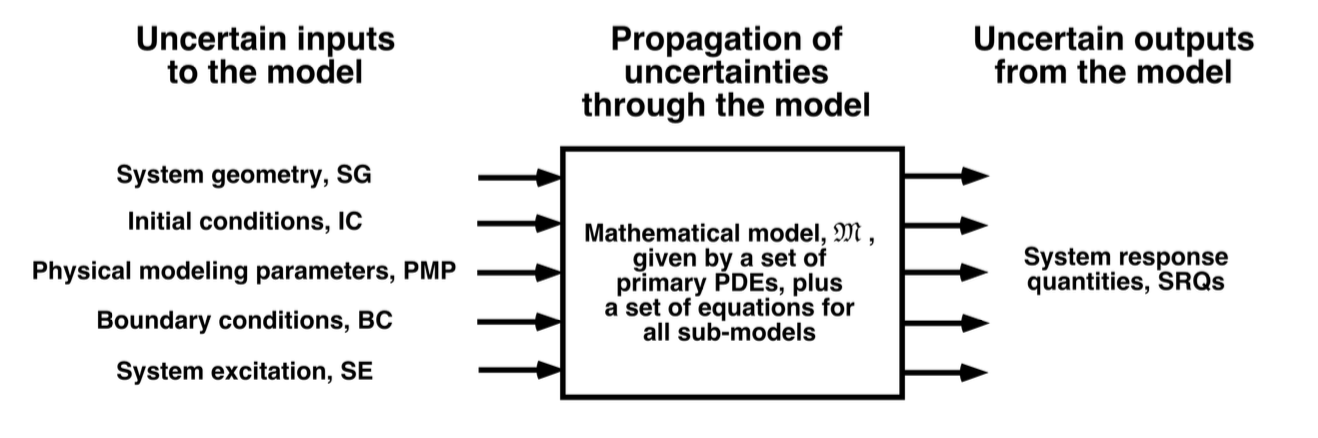
\includegraphics[width=\linewidth]{v_and_v_uq}
  \caption{Uncertainty Quantification \cite{oberkampf}}
  \label{fig:ober}
\end{figure}

In general, we define $u(Y)$ to be
a response as a function of the input space $Y = (y_1,\ldots,y_n,\ldots,y_N)$ where $y_n$ is a single
uncertain input
parameter to the model, $n$ is an index spanning the number of inputs, and $N$ is the total number of inputs.
Uncertain input parameters can include any of the inputs to the simulation.
We assume each response to be a scalar, integrated quantity.  In the event
the output is a vector or field quantity, each element can be considered as a distinct scalar response.
\emph{Models} are mathematical equations used to obtain the response $u(Y)$, and \emph{solvers} or
\emph{simulations} are numerical algorithms used to solve models.

Using our examples above, for neutronics calculations $Y$ might include nuclear cross sections, geometry
parameters, and sources, while $u(Y)$ could be $k$-effective or the neutron flux at a particular location of
interest.  For fuels performance calculations, $Y$ might entail thermal conductivity of various parameters,
geometric construction parameters, moderator inlet temperatures, and so forth.  $u(Y)$ could be peak clad
temperature, maximum fuel centerline temperature, clad elongation, percent fission gas released, and so on.

\subsection{Uncertain Inputs}
Essential to using simulation models is understanding the possibility that significant uncertainties exist in
the inputs.  These could be aleatoric uncertainties due to intrinsic randomness in the inputs, or epistemic
uncertainties due to model imperfections or lack of knowledge.  
For example, quantum behaviors or Brownian motion often provide non-deterministic sources of aleatoric uncertainty.
Further, the simulation itself might be solved through non-deterministic methods such as Monte Carlo sampling,
in which case the random seed acts as an uncertain input.  Examples of epistemic uncertainties include initial
or boundary conditions that can only be controlled to some finite level, such as manufacturing tolerances,
temperature and pressure, and so forth.
Each of these aleatoric and epistemic uncertainties has some
distribution defining the likelihood of an input to have a particular value.  Sometimes these distributions
are known; often, they can only be approximated.  These distributions might be
assumed or constructed from experiment; for our work, we will assume distributions are given, and that the given 
distributions are accurate.  

The distribution of input likelihoods is the probability distribution function (PDF) $\rho_n(y_n)$.  
An integral over any portion of the input space of the PDF provides the probability that the input's value
is within that portion.
We require
\begin{equation}
  \int_a^b \rho_n(y_n) d\ y_n = 1,
\end{equation}
where $a$ and $b$ are the minimum and maximum values $y_n$ can take (possibly infinite).  In other words, the
probability of finding the input between $a$ and $b$ is 100\%; similarly, we can say the value of the input
lies between $a$ and $b$ almost surely.

\subsection{Multidimensional Input Spaces}
% multidimensional
When there are more than one uncertain input, the combination of distributions for these inputs make up an
uncertainty space $\Omega$. $\Omega$ is a part of the probability space $(\Omega,\sigma,\rho)$, where $\Omega$
is the set of all possible outcomes, $\sigma$ is the set of events $\omega$, and $\rho$ is the probability function for
the space.  The dimensionality of $\Omega$ is $N$,
the number of uncertain input variables.  The probability of any event in the input space occurring is given
by an integral of the joint-probability distribution $\rho(Y)$, still enforcing
\begin{equation} \label{eq:joint pdf}
  \int_{a_1}^{b_1}\cdots\int_{a_N}^{b_N} \rho(Y) dy_1\cdots dy_N = 1.
\end{equation}
For clarity, we define multidimensional integral operator
\begin{equation}\label{eq: no rho}
  \int_\Omega (\cdot)dY\equiv \int_{a_1}^{b_1}\cdots\int_{a_N}^{b_N} (\cdot) dy_1\cdots dy_N,
\end{equation}
so that Eq. \ref{eq:joint pdf} can be written
\begin{equation}
  \int_\Omega \rho(Y) dY = 1.
\end{equation}
The function $u(Y)$ maps realizations ($\omega$) from the input space $\Omega$ to a real-valued response.
That is, for each input variable $y_n$, a realization is taken by selecting a single value from the
distribution of $y_n$, which gives a single input value $y_n(\omega)$.  Taking a single realization of each of
the distributed input parameters yields a full input realization $Y(\omega)=(y_1(\omega),\cdots,y_N(\omega))$,
which can be used as inputs for
$u(Y)$ to obtain a realization of the response $u(Y(\omega))$.  To simplify notation, in general the
dependency of a realization on $\omega$ will be omitted and referred to as \emph{sampling} or \emph{taking a
realization}.

% correlation
\subsection{Correlation and the Karhunen-Loeve expansion}\label{sec:KL}
We note the possibility that multiple inputs may be correlated with each other.  When inputs are not
independent, the joint probability distribution is not the product of each individual probability distribution
distribution.  When this is the case, each distribution cannot be sampled independently, and this
creates complications for many of the sampling strategies presented in this work.  

Using input space mapping, however, a surrogate orthogonal input space can be
constructed.  This surrogate space is functionally identical to the original for our purposes.
There are mathematical approaches to decoupling input parameters through surrogate
spaces.  In particular, using principle component analysis (or Karhunen-Loeve expansion
\cite{karhunen} for discrete inputs), the covariance matrix for the distributed input parameters
can be used to construct a multidimensional
standard Gaussian normal distribution, whose components are all orthogonal.
As a result, we only consider independent variables in this work, as dependent variables can
be decoupled through this surrogate mapping process.


\section{Uncertainty Quantification}
% introduction
The purpose of uncertainty quantification is to propagate the uncertainties present in the input space of a
model through that model and comprehend their effects on the output responses.  This is desirable because
single-realization simulations give a very limited view of real-life operation.  In traditional simulations, a
single value for each input variable results in a single value for the response.  When performing uncertainty
quantification, a range of values for each input results in a range of response values.  To quantify the
distribution of the output response, often statistical moments are used, including the mean, variance,
skewness, and kurtosis.

\subsection{Statistical Moments}\label{sec:stat moments}
The four most basic statistical moments used in describing probability distributions are the mean, variance,
skewness, and (excess) kurtosis.
The mean ($\mu$) provides the expected value of the response, or generally the most probable
value for the response.  The variance ($\sigma^2$) establishes the spread of the response, or the distance response values
have from the mean on average.  The standard deviation of the response is given by the square root of the
variance, and provides a useful metric to determine the probability of finding a response value within a
range.  For instance, Chebyshev's inequality \cite{chebyshevineq} says $1-1/k^2$ of a distribution's values
are within $k$ standard deviations from the mean.  This is true whenever the mean and variance can be
defined.  Table
\ref{tab:cheby stdev} shows the minimum percent of the response covered by including multiples of the
standard deviation from the mean.

Some distributions are much more restrictive than Chebyshev's inequality requires.  For instance, we 
show a similar table for a normal Gaussin distribution in Table \ref{tab:norm stdev}.  Fig. \ref{fig:stdev pct}
shows the same information graphically.
\begin{table}[htb]
  \centering
  \begin{tabular}{c c}
  Number of Std. Dev. & Percent of Values \\ \hline
  1 & 0 \\
  $\sqrt{2}$ & 50 \\
  2 & 75 \\
  3 & 88.89 \\
  4 & 93.75 \\
  5 & 96 \\
  10 & 99
  \end{tabular}
  \caption{Percentage of Values within $k$ standard deviations for general distributions}
  \label{tab:cheby stdev}
\end{table}
\begin{table}[htb]
  \centering
  \begin{tabular}{c c}
  Number of Std. Dev. & Percent of Values \\ \hline
  1 & 68.3 \\
  2 & 95.45 \\
  3 & 99.73 \\
  4 & 99.994 \\
  \end{tabular}
  \caption{Percentage of Values within $k$ standard deviations for Gaussian normal}
  \label{tab:norm stdev}
\end{table}
\begin{figure}[H]
  \centering
  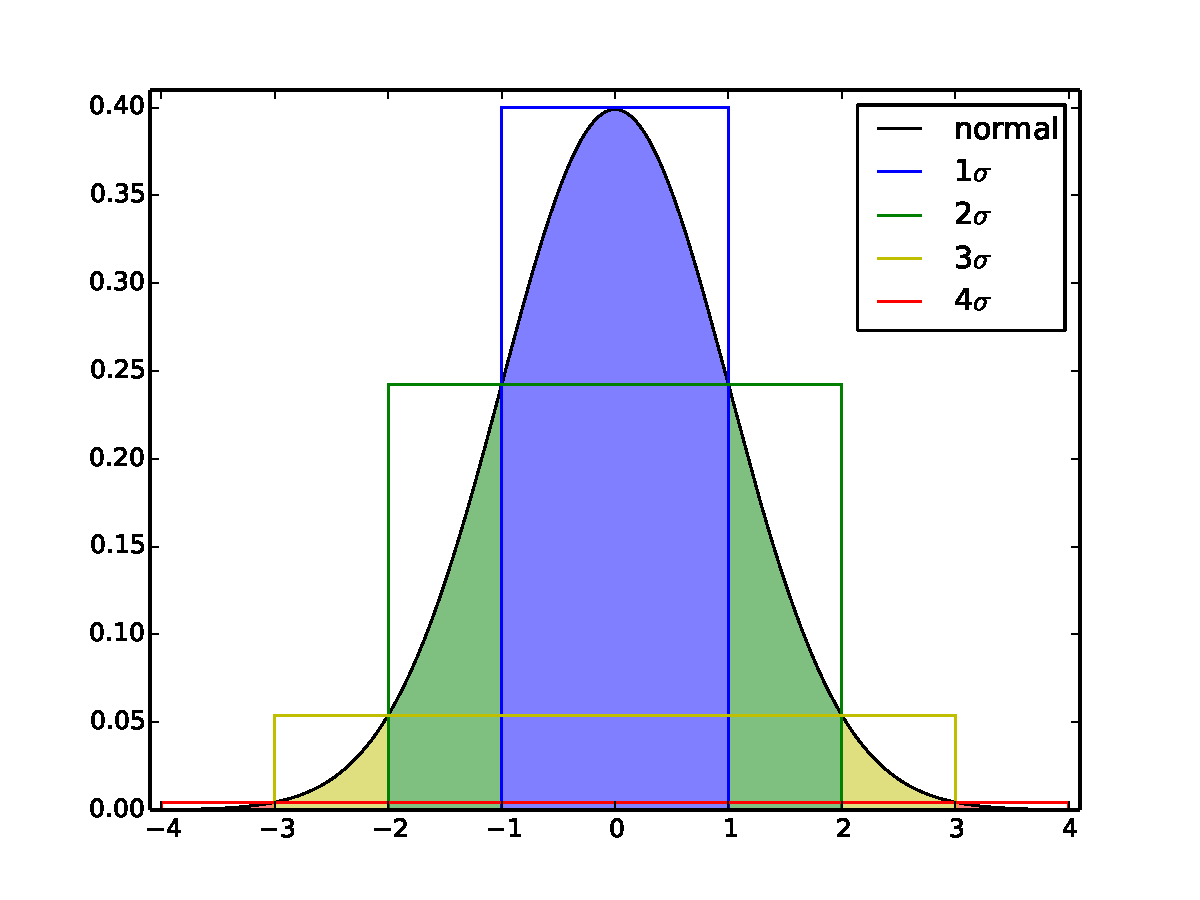
\includegraphics[width=0.7\linewidth]{stdev_pct}
  \caption{Standard Deviations of Normal Gaussian Distribution}
  \label{fig:stdev pct}
\end{figure}
Higher order moments, skewness ($\gamma_1$) and kurtosis ($\gamma_2$), describe the asymmetry and "tailedness"
of the response distribution respectively.  The more asymmetric the distribution, the
higher the skewness is.  For example, a Gaussian normal distribution has zero skewness,
and skewness is introduced to a Beta distribution by allowing $\alpha\neq\beta$.
Kurtosis is more complicated in its interpretation, but in general kurtosis provides an idea
of how much of the variance is contributed by extreme deviations from the mean.  The kurtosis
of a Guassian normal distribution is 3.  This leads to the definition of excess kurtosis,
which is 3 less than the traditional kurtosis.  

An example of similar distributions with different moments is
given in Figure \ref{fig:change moments}.  The mean shifts the entire distribution, the variance spreads the
distribution, the skewness measures asymmetry, and the kurtosis measures tailedness.  In each case, the blue
is a ``standard'' distribution, and the red demonstrates increasing the indicated statistical moment.
\begin{figure}[H]
  \centering
  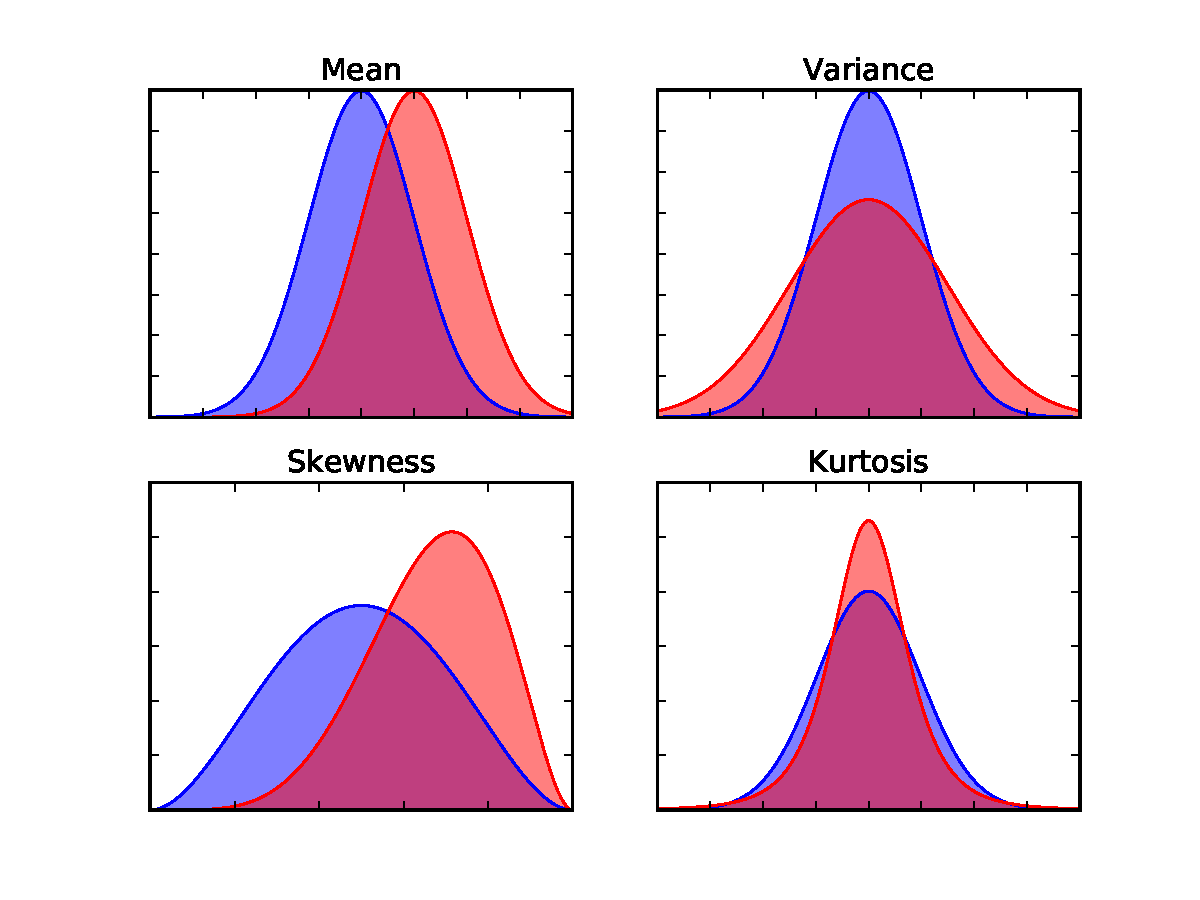
\includegraphics[width=0.7\linewidth]{change_stats}
  \caption{Visual Representation of Statistical Moments}
  \label{fig:change moments}
\end{figure}

While both skewness and kurtosis provide insight to the distribution of responses,
most uncertainty quantification is centered on second-order metrics.
Second-order uncertainty quantification seeks for the mean and variance of
the perturbed response.  Mathematically, the mean ($\mu$) of a model is the first moment,
\begin{equation}
  \mu = \expv{u(Y)} = \int_\Omega u(Y) dY,
\end{equation}
and the variance ($\sigma^2$) is the second moment less the square of the first,
\begin{equation}
  \sigma^2 = \expv{u(Y)^2} - \expv{u(Y)}^2 = \int_\Omega u(Y)^2 dY - \mu^2.
\end{equation}
 
Another use for uncertainty quantification is understanding the sensitivity of the output responses to the
uncertain inputs; that is, determining how responses change as a function of changes in the input space.  At
the most primitive level, linear sensitivity of the mean of a response to an input is the derivative of the response
with respect to the input.  Sensitivities can be either local to a region in the input space or global
to the entire space.

There are two chief methods to define sensitivity.  One of the most typical sensitivities
is mean to mean; that is, the rate of change in the value of the response as a function of changes in the
input values.  This metric is most useful what attempting to maximize or minimize a response value by changing
input parameters.  The second method is variance to variance, or the rate of change in the variance of the
response as a function of changes in the variance of an input.  This is useful when trying to mitigate the
spread of possible response values.  If there is a possibility of a response having an undesirable value,
knowing the variance-variance sensitivity helps in identifying which inputs need to have their variance
reduced to prevent the undesirable value from occurring.

\subsection{After Uncertainty Quantification}
Once the response distribution is well-understood through statistical moments and sensitivities, 
further analysis
and decisions can be made.  For example, one post-uncertainty quantification analysis is \emph{limit
surface} definition and \emph{failure probability}.  In this type of analysis, a criteria is given that determines
a ``success'' and ``failure'' condition for a response.  For instance, in the simulation of a
material undergoing stress during heating, a failure condition could be whether the material
buckles during the simulation.  The limit surface search seeks to determine what portion of the
input space results in response failures, and what portion to successes, and define the hypersurfaces dividing
successes and failures.  Figure \ref{fig:lss} shows a sample limit surface search sampling, and Figure
\ref{fig:lss fail} shows the surface between success and failure regions \cite{raven}.  

\begin{figure}[htb]
  \centering
  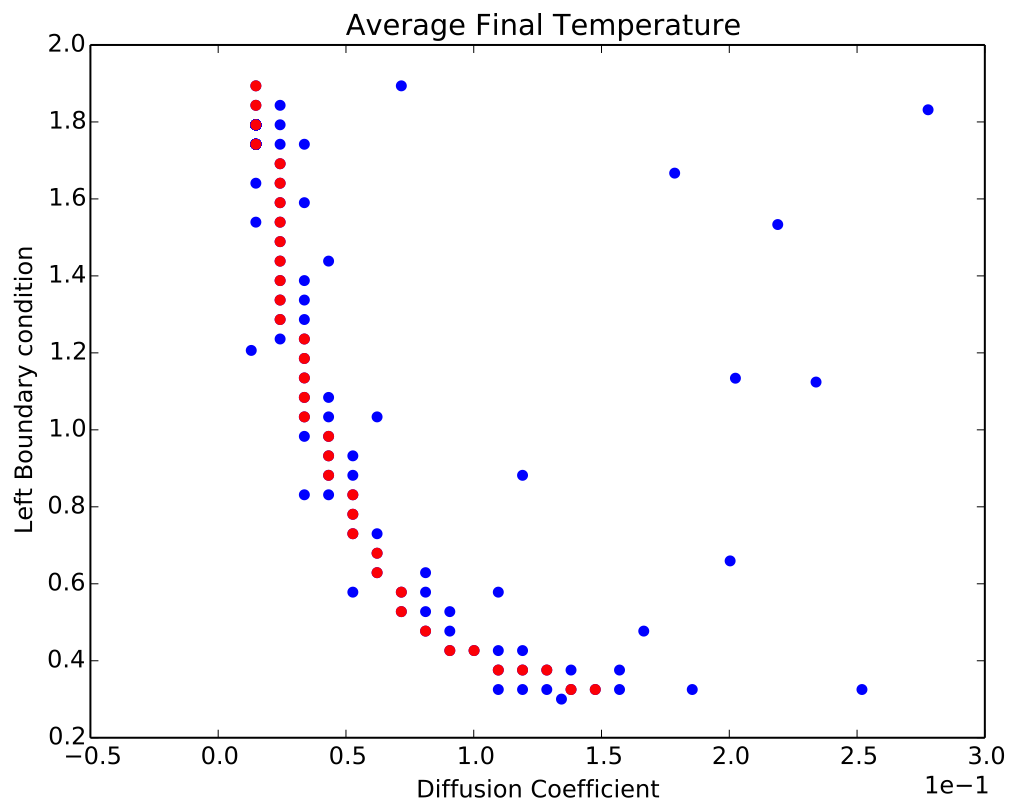
\includegraphics[width=0.5\linewidth]{lss}
  \caption{Limit Surface Sampling \cite{raven}}
  \label{fig:lss}
\end{figure}
\begin{figure}[htb]
  \centering
  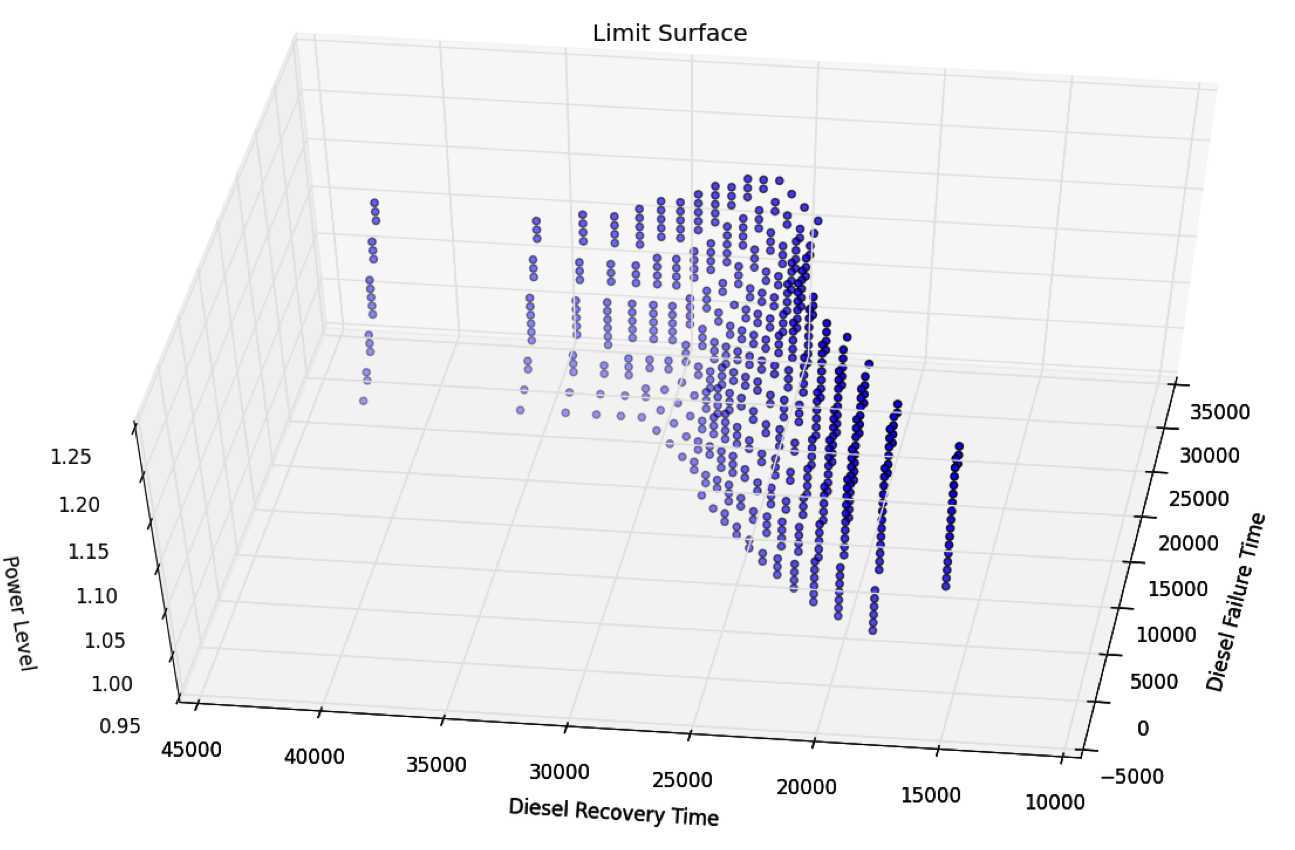
\includegraphics[width=0.7\linewidth]{lss_fail}
  \caption{Limit Surface and Failure Regions \cite{raven}}
  \label{fig:lss fail}
\end{figure}

After a limit surface search, optimization can be performed, which gives
some criteria for ideal operation and searches the success space for optimal inputs.  For example,
if alloy compositions are the inputs for the stress and heat material mentioned earlier, optimization
can help find the least expensive alloy that won't buckle in the conditions given by the simulation.

Another post-uncertainty quantification calculation is to make use of sensitivity information to determine
the inputs that could benefit from reduced variance to reduce the variance of the response in turn.
If some inputs have minimal impact on variance in the output, they don't need the same level of care
in manufacturing as other inputs.  For example, consider the construction of a commercial nuclear power
reactor.  If the material properties and geometry of the reflector have a much smaller impact on the operation
variance than the fuel content and geometry of the fuel pellets, the most naive cost-effective way to control
variance is to decrease margins in fuel manufacturing instead of reflector construction.  While this example
seems readily evident, often engineering intuition can be informed by uncertainty quantification and
sensitivity analysis.

\subsection{Analytic Uncertainty Quantification}
For some models, there exists analytic techniques for propagation of uncertainty.  One of these is the
so-called \emph{sandwich formula}, often referred to as \emph{standard propagation of error} \cite{sandwich}.
Assuming independent input parameters (see section \ref{sec:KL}), the standard deviation $\sigma_u$ of $u(Y)$
is given as
\begin{equation}
  \sigma^2_u = \sum_{n=1}^N \qty(\pdv{u(Y)}{y_n})^2\sigma_{y_n}^2,
\end{equation}
where $\sigma_{y_n}$ is the standard deviation of uncertain input $y_n$.  This approximation is limited to the
linear characteristics of the gradient of $u(Y)$, and so is useful especially when the standard deviation of
the inputs are small compared to the partial derivatives \cite{sandwich2}.

For models with gradients that are simple to calculate accurately (and sufficiently small input
uncertainties), this formula is very effective at propagating error.  However, computing or estimating such
gradients accurately for complex models is prohibitive, and leads to numerical approaches to uncertainty
quantification, as we discuss in this work.


\subsection{Uncertainty Quantification Techniques}
There are several common tools used for uncertainty quantification when analytic analysis is not possible or
not practical.
These include stochastic methods such as Monte Carlo sampling, deterministic methods such as Grid sampling,
and mixed methods such as Latin Hypercube sampling (LHS). We discuss each here and show examples of the
sampling strategies.

\subsection{Monte Carlo}
The Monte Carlo method (MC) \cite{mc} has been used formally since the 1930s as a tool to explore possible outcomes
in uncertain models.  Nuclear physicist Enrico Fermi used the method in his work with neutron moderation in
Rome \cite{mcfermi}.  In its simplest form, MC involves randomly picking realizations from a set of
possibilities, then statistically collecting the results.  In uncertainty quantification, Monte Carlo can be
used to sample realizations in the input space based on the joint probability distribution.  These
realizations are then run through the model solver, and the collection of
response realizations is analyzed to determine its moments.

The mean of a response is determined by MC using the unweighted average of samples collected:
\begin{equation}
  \expv{u(Y)} = \frac{1}{M}\sum_{m=1}^M \qty(u(Y(\omega_m))) + \epsilon_M^{\text{MC}},
\end{equation}
where $Y(\omega_m)$ is a realization randomly chosen based on $\rho(Y)$, and $M$ is the total number of samples taken.
The error in the approximation diminishes with the root of the number of samples taken,
\begin{equation}
  \epsilon_M^{\text{MC}} \propto \frac{1}{\sqrt{M}}.
\end{equation}
The second moment is similarly approximated as
\begin{equation}
  \expv{u(Y)^2} \approx \frac{1}{M}\sum_{m=1}^M \qty(u(Y(\omega_m))^2).
\end{equation}
The standard deviation (root of the variance) converges similarly to the mean for Monte Carlo methods.  There
are many tools that can be used to improve Monte Carlo sampling \cite{mcvarred}\cite{mcnpvarred}; we restrict
our discussion to traditional analog Monte Carlo sampling.

Monte Carlo has long been a gold standard for uncertainty quantification because of its consistency.  Monte
Carlo will always resolve the response statistics given a sufficient number of samples.  Additionally, the
convergence of Monte Carlo is largely agnostic of the input space dimensionality, a feature not shared by the
Grid sampling method.

The drawback to Monte Carlo sampling also centers on its consistency.  The error in analog Monte Carlo can only be
consistently reduced by drastically increasing the number of evaluations solved.  While coarse estimates are
inexpensive to obtain, high precision takes a great deal of effort to converge.
Figure \ref{fig:mc sample}
shows Monte Carlo sampling of a two-dimensional input space, and Figure \ref{fig:mc prob} shows the
probability weight of the sampled points \cite{raven}.

\begin{figure}[H]
  \centering
  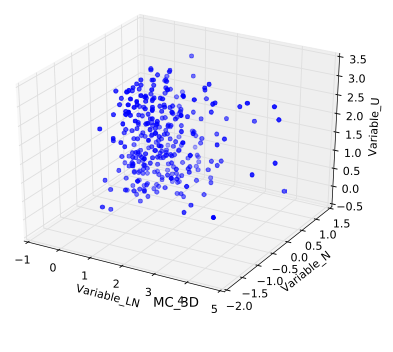
\includegraphics[width=0.5\linewidth]{mc_sample}
  \caption{Example Monte Carlo Samples \cite{raven}}
  \label{fig:mc sample}
\end{figure}
\begin{figure}[H]
  \centering
  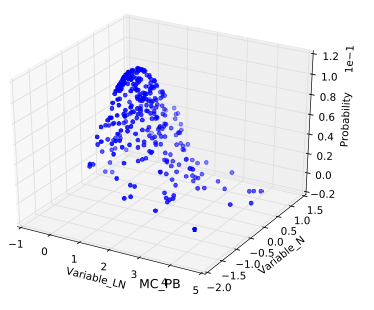
\includegraphics[width=0.5\linewidth]{mc_prob}
  \caption{Example Monte Carlo Probabilities \cite{raven}}
  \label{fig:mc prob}
\end{figure}

\subsection{Grid}
One of the drawbacks of Monte Carlo is lack of control over points sampled.
An alternative is using a structured orthogonal grid.  In this strategy, the input space is
divided into hypervolumes that are equal in volume either in the input space or in uncertainty space.  For
demonstration, we first consider a one-dimensional case with a single normally-distributed variable $y$ with mean
$\mu$ and standard deviation $\sigma$.  If the input space is divided into equal volumes in the input space,
a lower and upper bound are determined,
then nodes are selected on the ends and equally spaced throughout.  If the input space is
divided into equal probability volumes, nodes are selected to be equidistant along the cumulative distribution
function (CDF).  This assures that the volume between each set of nodes has equal probability.  See Figure
\ref{fig:grid samp}, in which both equal in value and equal in CDF grid spacing is applied to a standard Gaussian
normal distribution.
\begin{figure}[htb]
  \centering
  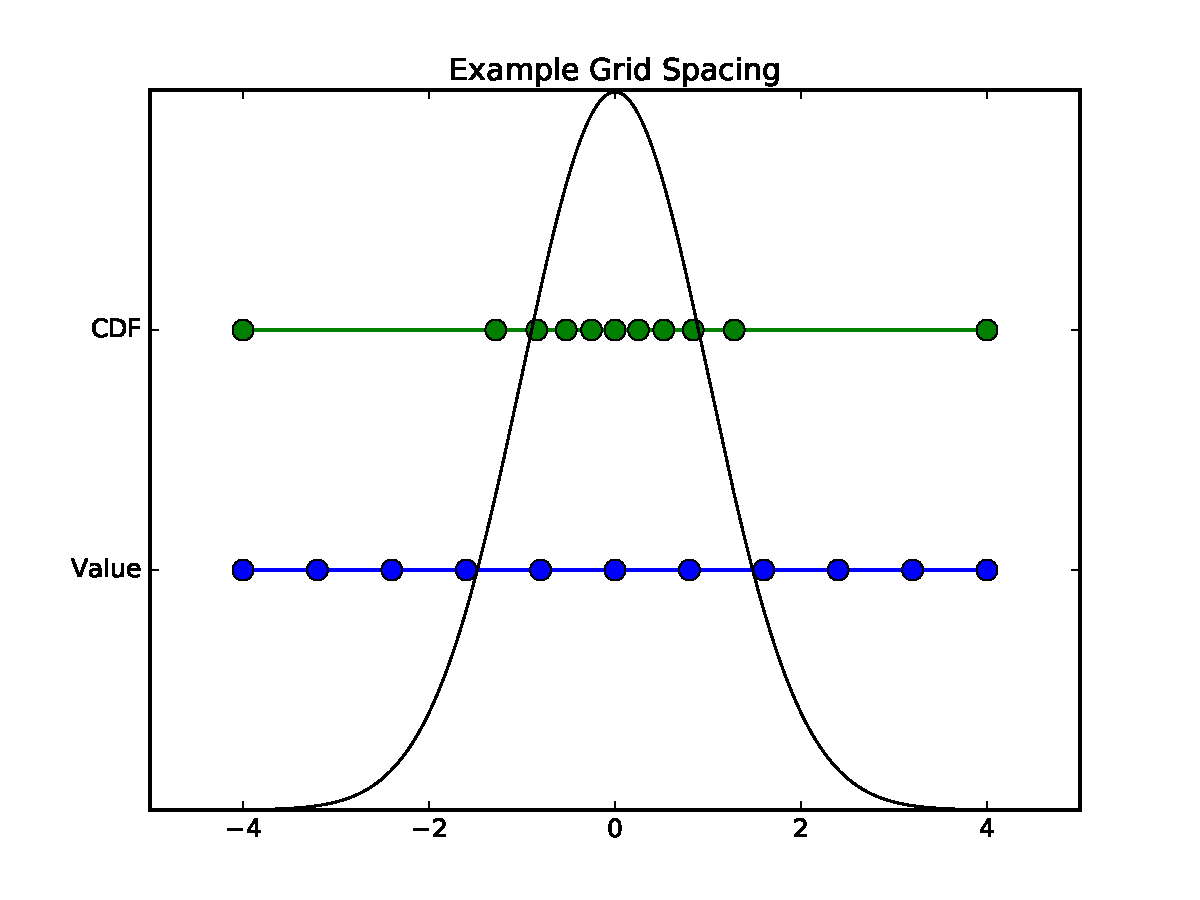
\includegraphics[width=0.7\linewidth]{grid_spacing}
  \caption{Grid Sampling}
  \label{fig:grid samp}
\end{figure}
In multidimensional input spaces, the tensor product of each grid is taken to result in the full grid.

Since the grid nodes are user-defined, approximating integrals are slightly more complicated than in the Monte
Carlo space.  The mean is approximated by
\begin{equation}
  \expv{u(Y)} = \int_\Omega u(Y) dY \approx \sum_{m=1}^M w_m u(Y(\omega_m)),
\end{equation}
where $m$ iterates over each node in the grid, $Y(\omega_m)$ is the multidimensional input realization at grid node $m$, and
$w_m$ is a probability weight determined by the volume of probability represented by the grid node.  In grids
constructed by CDF, all $w_m$ are of the same value, while in grids spaced equally by value, $w_m$ can vary
significantly.  Similarly, the second moment is approximated by
\begin{equation}
  \expv{u(Y)^2} = \int_\Omega u(Y)^2 dY \approx \sum_{m=1}^M w_m u(Y(\omega_m))^2.
\end{equation}

An advantage to grid sampling is its regular construction, which can give more clarity to how a response
behaves throughout the input space.  However, the grid construction suffers greatly from the curse of
dimensionality, which makes it inefficient for input spaces with large dimensionality.
Figure \ref{fig:grid sample}
shows Grid sampling of a two-dimensional input space, and Figure \ref{fig:grid prob} shows the
probability weight of the sampled points \cite{raven}.

\begin{figure}[H]
  \centering
  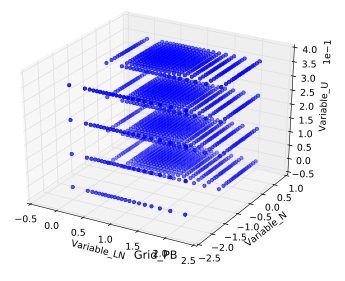
\includegraphics[width=0.5\linewidth]{grid_sample}
  \caption{Example Grid Samples \cite{raven}}
  \label{fig:grid sample}
\end{figure}
\begin{figure}[H]
  \centering
  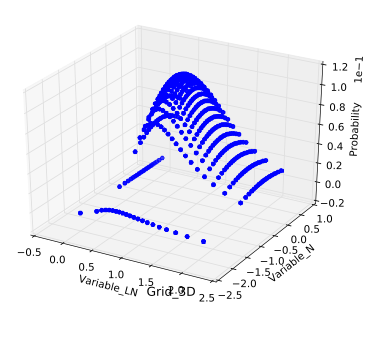
\includegraphics[width=0.5\linewidth]{grid_prob}
  \caption{Example Grid Probabilities \cite{raven}}
  \label{fig:grid prob}
\end{figure}


\subsection{LHS}
A cross between Monte Carlo and Grid sampling strategies, the Latin Hypercube Sampling (LHS) strategy 
is a sampling tool used to reduce
the total samples needed without significantly sacrificing integration quality \cite{lhs}.  In LHS, the input
space is also divided into a grid just as in the Grid sampling strategy.  However, unlike Grid sampling, only
one sample is taken per hyperplane; that is, for any of the input variables, there is only one sample taken
between each of the one-dimensional nodes.  Once a hypervolume is selected to take a sample, the exact
point is selected by random sampling in the probability space within the hypervolume.
Figure \ref{fig:lhs sample}
shows lhs sampling of a two-dimensional input space, and Figure \ref{fig:lhs prob} shows the
probability weight of the sampled points \cite{raven}.

\begin{figure}[H]
  \centering
  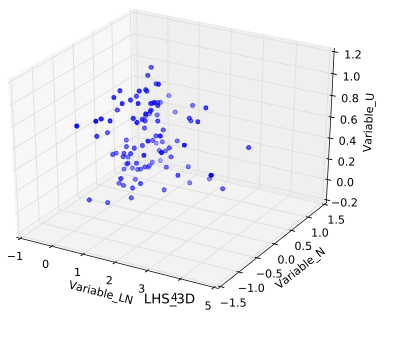
\includegraphics[width=0.5\linewidth]{lhs_sample}
  \caption{Example LHS Samples \cite{raven}}
  \label{fig:lhs sample}
\end{figure}
\begin{figure}[H]
  \centering
  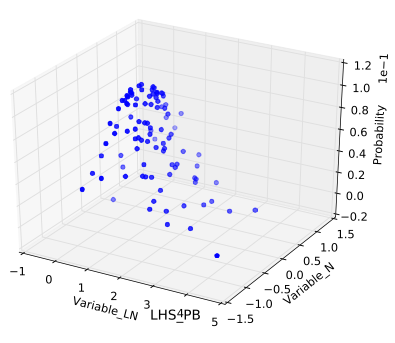
\includegraphics[width=0.5\linewidth]{lhs_prob}
  \caption{Example LHS Probabilities \cite{raven}}
  \label{fig:lhs prob}
\end{figure}

As in the Grid method, the weight of each sample is the probability volume of the hypervolume it represents.
While LHS has been a boon to computational researchers due to its low sample size, it struggles to resolve
responses with significant nonlinear shape.  Because only a small portion of the input space is used to obtain
the response statistics, there is a risk of missing important response features that may include
high-probability spaces.

\section{Conclusion}
Monte Carlo, Grid, and LHS sampling are all useful tools in uncertainty quantification.  Each one, however,
also has weak points that make it undesirable for some responses.  Monte Carlo tends to be slow in converging
to high-order accuracy, Grid suffers greatly from the curse of dimensionality, and LHS relies on
slowly-changing responses.  In the remainder of this work we explore advanced UQ methods to improve on these
three standard techniques.

 % 2
% Chapter Template

\chapter{Methods: Stochastic Collocation for Generalized Polynomial Chaos} % Main chapter title

\label{ch:methods scgpc} % Change X to a consecutive number; for referencing this chapter elsewhere, use \ref{ChapterX}

\lhead{Chapter 2. \emph{Methods: Collocation for Polynomial Chaos}} % Change X to a consecutive number; this is for the header on each page - perhaps a shortened title

%----------------------------------------------------------------------------------------
%	SECTION: INTRO
%----------------------------------------------------------------------------------------

\section{Introduction}
In this chapter we describe several common and novel uncertainty quantification methods and their applications.
We begin
by discussing the principles of input spaces and responses, and define terminology used in this work.  Next we
discuss uncertainty quantification at a high level, and describe several common uncertainty quantification
tools.  Finally, we explore Stochastic Collocation for generalized Polynomial Chaos (SCgPC), an advanced
uncertainty quantification technique.

% inputs and outputs
Many simulation models are algorithms constructed to solve partial differential equations, often in two or
three spatial dimensions and possibly time.  The inputs to these models include boundary conditions, material
properties, tuning parameters, and so forth.  The outputs are responses, either data fields or
scalar values.  The responses are used to inform decision-making processes.  For example, a neutronics
simulation in nuclear engineering takes materials, geometries, and boundary conditions as inputs, and yields
neutron flux and the neutron multiplication factor $k$ as responses.  Similarly, a fuels performance code
takes materials, geometries, and power shapes as inputs and yields stresses, strains, and temperature profiles
as outputs.  Figure \ref{fig:ober} is an example of this workflow \cite{oberkampf}.
\begin{figure}
  \centering
  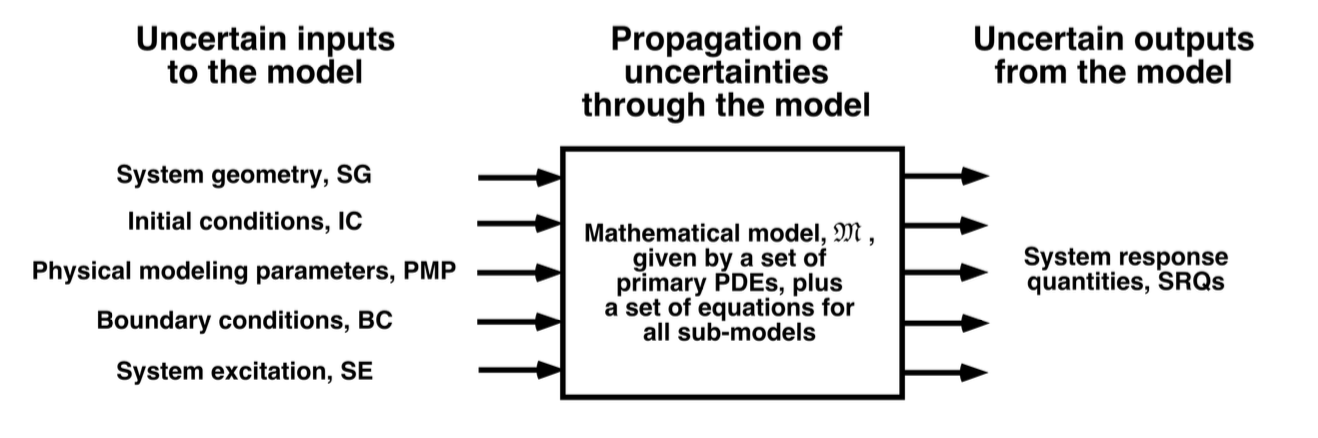
\includegraphics[width=\linewidth]{v_and_v_uq}
  \caption{Uncertainty Quantification \cite{oberkampf}}
  \label{fig:ober}
\end{figure}

In general, we define $u(Y)$ to be
a response as a function of the input space $Y = (y_1,\ldots,y_n,\ldots,y_N)$ where $y_n$ is a single
uncertain input
parameter to the model, $n$ is an index spanning the number of inputs, and $N$ is the total number of inputs.
Uncertain input parameters can include any of the inputs to the simulation.
We assume each response to be a scalar, integrated quantity.  In the event
the output is a vector or field quantity, each element can be considered as a distinct scalar response.
\emph{Models} are mathematical equations used to obtain the response $u(Y)$, and \emph{solvers} or
\emph{simulations} are numerical algorithms used to solve models.

Using our examples above, for neutronics calculations $Y$ might include nuclear cross sections, geometry
parameters, and sources, while $u(Y)$ could be $k$-effective or the neutron flux at a particular location of
interest.  For fuels performance calculations, $Y$ might entail thermal conductivity of various parameters,
geometric construction parameters, moderator inlet temperatures, and so forth.  $u(Y)$ could be peak clad
temperature, maximum fuel centerline temperature, clad elongation, percent fission gas released, and so on.

\subsection{Uncertain Inputs}
Essential to using simulation models is understanding the possibility that significant uncertainties existing in
the inputs.  These could be aleatoric uncertainties due to intrinsic randomness in the inputs, or epistemic
uncertainties due to model imperfections or lack of knowledge.  
For example, quantum behaviors or Brownian motion often provide non-deterministic sources of aleatoric uncertainty.
Further, the simulation itself might be solved through non-deterministic methods such as Monte Carlo sampling,
in which case the random seed acts as an uncertain input.  Examples of epistemic uncertainties include initial
or boundary conditions that can only be controlled to some finite level, such as manufacturing tolerances,
temperature and pressure, and so forth.
Each of these aleatoric and epistemic uncertainties has some
distribution defining the likelihood of an input to have a particular value.  Sometimes these distributions
are known; often, they can only be approximated.  These distributions might be
assumed or constructed from experiment; for our work, we will assume distributions are given, and that the given 
distributions are accurate.  The
input likelihood distribution is the probability distribution function (PDF) $\rho_n(y_n)$.  
An integral over any portion of the input space of the PDF provides the probability that the input's value
is within that portion.
We require
\begin{equation}
  \int_a^b \rho_n(y_n) d\ y_n = 1,
\end{equation}
where $a$ and $b$ are the minimum and maximum values $y_n$ can take (possibly infinite).  In other words, the
probability of finding the input between $a$ and $b$ is 100\%; similarly, we can say the value of the input
lies between $a$ and $b$ almost surely.

\subsection{Multidimensional Input Spaces}
% multidimensional
When there are more than one uncertain input, the combination of distributions for these inputs span an
uncertainty space $\Omega$. $\Omega$ is a part of the probability space $(\Omega,\sigma,\rho)$, where $\Omega$
is the set of all possible outcomes, $\sigma$ is the set of events $\omega$, and $\rho$ is the probability function for
the space.  The dimensionality of $\Omega$ is $N$,
the number of uncertain input variables.  The probability of any event in the input space occurring is given
by an integral of the joint-probability distribution $\rho(Y)$, still enforcing
\begin{equation} \label{eq:joint pdf}
  \int_{a_1}^{b_1}\cdots\int_{a_N}^{b_N} \rho(Y) dy_1\cdots dy_N = 1.
\end{equation}
For clarity, we define multidimensional integral operator
\begin{equation}
  \int_\Omega (\cdot)dY\equiv \int_{a_1}^{b_1}\cdots\int_{a_N}^{b_N} (\cdot) dy_1\cdots dy_N,
\end{equation}
so that Eq. \ref{eq:joint pdf} can be written
\begin{equation}
  \int_\Omega \rho(Y) dY = 1.
\end{equation}
The function $u(Y)$ maps realizations ($\omega$) from the input space $\Omega$ to a real-valued response.
That is, for each input variable $y_n$, a realization is taken by selecting a single value from the
distribution of $y_n$, which gives a single input value $y_n(\omega)$.  Taking a single realization of each of
the distributed input parameters yields a full input realization $Y(\omega)=(y_1(\omega),\cdots,y_N(\omega))$,
which can be used as inputs for
$u(Y)$ to obtain a realization of the response $u(Y(\omega))$.  To simplify notation, in general the
dependency of a realization on $\omega$ will be omitted and referred to as \emph{sampling} or \emph{taking a
realization}.

% correlation
\subsection{Correlation and the Karhunen-Loevre expansion}\label{sec:kl}
We note the possibility that multiple inputs may be correlated with each other.  When inputs are not
independent, the joint probability distribution is not the product of each individual probability distribution
distribution.  When this is the case, each distribution cannot be sampled independently, and this
creates complications for many of the sampling strategies presented in this work.  

Using input space mapping, however, a surrogate orthogonal input space can be
constructed.  This surrogate space is functionally identical to the original for our purposes.
There are mathematical approaches to decoupling input parameters through surrogate
spaces.  In particular, using principle component analysis (or Karhunen-Loeve expansion
\cite{karhunen} for discrete inputs), the covariance matrix for the distributed input parameters
can be used to construct a multidimensional
standard Gaussian normal distribution, whose components are all orthogonal.
As a result, we only consider independent variables in this work, as dependent variables can
be decoupled through this surrogate mapping process.


\section{Uncertainty Quantification}
% introduction
The purpose of uncertainty quantification is to propagate the uncertainties present in the input space of a
problem through the model and comprehend their effects on the output responses.  In traditional simulations, a
single value for each input variable results in a single value for the response.  When performing uncertainty
quantification, a range of values for each input results in a range of response values.  To quantify the
distribution of the output response, often statistical moments are used, including the mean, variance,
skewness, and kurtosis.
\subsection{Statistical Moments}
The mean provides the expected value of the response, or generally the most probable
value for the response.  The variance establishes the spread of the response, or the distance response values
have from the mean on average.  The standard deviation of the response is given by the square root of the
variance, and provides a useful metric to determine the probability of finding a response value within a
range.  For instance, Chebyshev's inequality \cite{chebyshevineq} says $1-1/k^2$ of a distribution's values
are within $k$ standard deviations from the mean.  This is true whenever the mean and variance can be
defined.  Table
\ref{tab:cheby stdev} shows the minimum percent of the response covered by expanding the range by multiples of the
standard deviation.
Some distributions are much more restrictive than Chebyshev's inequality requires.  For instance, we 
show a similar table for a normal Gaussin distribution in Table \ref{tab:norm stdev}.  Fig. \ref{fig:stdev pct}
shows the same information graphically.
\begin{table}[htb]
  \centering
  \begin{tabular}{c c}
  Number of Std. Dev. & Percent of Values \\ \hline
  1 & 0 \\
  $\sqrt{2}$ & 50 \\
  2 & 75 \\
  3 & 88.89 \\
  4 & 93.75 \\
  5 & 96 \\
  10 & 99
  \end{tabular}
  \caption{Percentage of Values within $k$ standard deviations for general distributions}
  \label{tab:cheby stdev}
\end{table}
\begin{table}[htb]
  \centering
  \begin{tabular}{c c}
  Number of Std. Dev. & Percent of Values \\ \hline
  1 & 68.3 \\
  2 & 95.45 \\
  3 & 99.73 \\
  4 & 99.994 \\
  \end{tabular}
  \caption{Percentage of Values within $k$ standard deviations for Gaussian normal}
  \label{tab:norm stdev}
\end{table}
\begin{figure}[H]
  \centering
  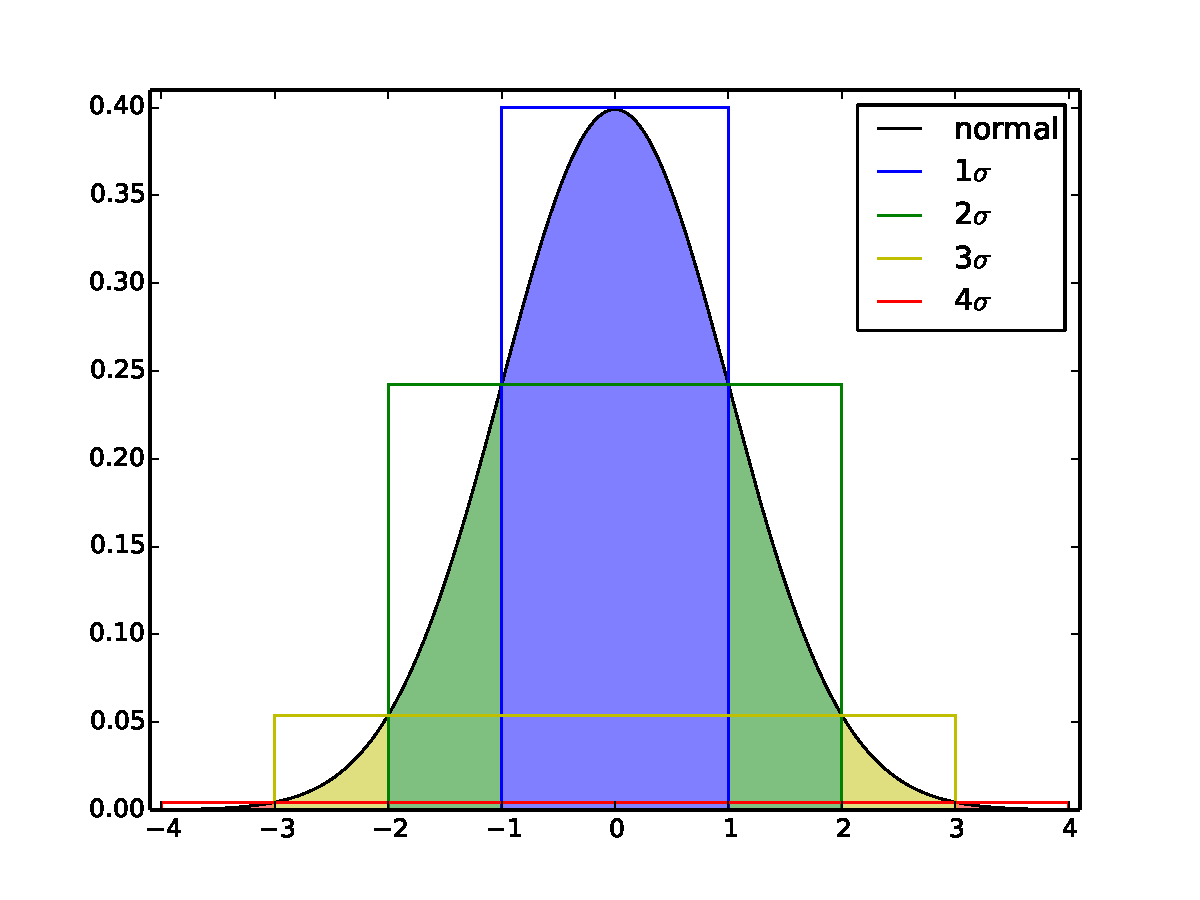
\includegraphics[width=0.7\linewidth]{stdev_pct}
  \caption{Standard Deviations of Normal Gaussian Distribution}
  \label{fig:stdev pct}
\end{figure}
Higher order moments, skewness and kurtosis, describe the asymmetry and "tailedness"
of the response distribution respectively.  The more asymmetric the distribution, the
higher the skewness is.  For example, a Gaussian normal distribution has zero skewness,
and skewness is introduced to a Beta distribution by allowing $\alpha\neq\beta$.
Kurtosis is more complicated in its interpretation, but in general kurtosis provides an idea
of how much of the variance is contributed by extreme deviations from the mean.  The kurtosis
of a Guassian normal distribution is 3.  This leads to the definition of excess kurtosis,
which is 3 less than the traditional kurtosis.

While both the skewness and kurtosis provide insight as to the distribution of reponses,
most uncertainty quantification is centered on second-order metrics.
Second-order uncertainty quantification seeks for the mean and variance of
the perturbed response.  Mathematically, the mean of a model is the first moment,
\begin{equation}
  \text{mean} = \expv{u(Y)} = \int_\Omega \rho(Y) u(Y) dY,
\end{equation}
and the variance is the second moment less the square of the first,
\begin{equation}
  \text{variance} = \expv{u(Y)^2} - \expv{u(Y)}^2 = \int_\Omega \rho(Y) u(Y)^2 dY - \text{mean}^2.
\end{equation}
 
Another use for uncertainty quantification is understanding the sensitivity of the output responses to the
uncertain inputs; that is, determining how responses change as a function of changes in the input space.  At
the most primitive level, linear sensitivity of a response mean to an input is the derivative of the response
with respect to the input.  Sensitivities can be both local to a region in the input space as well as global
to the entire problem.

In addition, there are two chief methods to define sensitivity.  One of the most typical sensitivities
is mean to mean; that is, the rate of change in the value of the reponse as a function of changes in the
input.  This metric is most useful what attempting to maximize or minimize a response value by changing
input parametrs.  The second method is variance to variance, or the rate of change in the variance of the
response as a function of changes in the variance of an input.  This is useful when trying to mitigate the
spread of possible response values.  If there is a possibility of a response having an undesirable value,
knowing the variance-variance sensitivity helps in identifying which inputs need to have their variance
reduced to prevent the undesirable value from occuring.

\subsection{After Uncertainty Quantification}
Once the response distribution is well-understood through statistical moments and sensitivities, 
further analysis
and decisions can be made.  For example, one post-uncertainty quantification analysis is limit
surface definition and failure probability.  In this analysis, a criteria is given that determines
a ``success'' and ``failure'' condition for a response.  For instance, in the simulation of a
material undergoing stress during heating, a failure condition could be whether the material
buckles during the simulation.  The limit surface search seeks to determine what portion of the
input space leads to failures, and what portion to successes, and define the hypersurfaces dividing
successes and failures.  After a limit surface search, optimization can be performed, which gives
some criteria for ideal operation and searches the success space for optimal inputs.  For example,
if alloy compositions are the inputs for the stress and heat material mentioned earlier, optimization
can help find the least expensive alloy that won't buckle in the conditions given by the simulation.

Another post-uncertainty quantification calculation is to make use of sensitivity information to determine
the inputs that could benefit from reduced variance to reduce the variance of the response in turn.
If some inputs have minimal impact on variance in the output, they don't need the same level of care
in manufacturing as other inputs.  For example, consider the construction of a commercial nuclear power
reactor.  If the material properties and geometry of the reflector have a much smaller impact on the operation
variance than the fuel content and geometry of the fuel pellets, the most naieve cost-effective way to control
variance are to decrease margins in fuel manufacturing instead of reflector construction.  While this example
seems readily evident, often engineering intuition can be surprised by uncertainty quantification and
sensitiviy analysis.

\subsection{Analytic Uncertainty Quantification}
For some models, there exists analytic techniques for propagation of uncertainty.  One of these is the
so-called \emph{sandwich formula}, often referred to as \emph{standard propagation of error} \cite{sandwich}.
Assuming independent input parameters (see section \ref{sec:KL}), the standard deviation $\sigma_u$ of $u(Y)$
is given as
\begin{equation}
  \sigma^2_u = \sum_{n=1}^N \qty(\pdv{u(Y)}{y_n})^2\sigma_{y_n}^2,
\end{equation}
where $\sigma_{y_n}$ is the standard deviation of uncertain input $y_n$.  This approximation is limited to the
linear characteristics of the gradient of $u(Y)$, and so is useful especially when the standard deviation of
the inputs are small compared to the partial derivatives \cite{sandwich2}.

For models with gradients that are simple to calculate accurately (and sufficiently small input
uncertainties), this formula is very effective at propagating error.  However, computing or estimating such
gradients accurately for complex models is prohibitive, and leads to numerical approaches to uncertainty
quantification, as we discuss in this thesis.


\subsection{Uncertainty Quantification Techniques}
There are several common tools used for uncertainty quantification when analytic analysis is not possible.
These include stochastic methods such as Monte Carlo sampling, deterministic methods such as Grid sampling,
and mixed methods such as Latin Hypercube sampling (LHS).  After describing these, we also consider advanced
uncertainty quantification techniques: generalized polynomial chaos expansion and high-dimension
model reduction.

\subsection{Monte Carlo}
The Monte Carlo method \cite{mc} has been used formally since the 1930s as a tool to explore possible outcomes
in uncertain models.  Nuclear physicist Enrico Fermi used the method in his work with neutron moderation in
Rome \cite{mcfermi}.  In its simplest form, Monte Carlo involves randomly picking realizations from a set of
possibilities, then statistically collecting the results.  In uncertainty quantification, Monte Carlo can be
used to sample points in the input space based on the joint probability distribution.  The collection of
points is analyzed to determine the moments of the response.

The mean of a response is determined using the unweighted average of samples collected:
\begin{equation}
  \expv{u(Y)} = \frac{1}{N}\sum_{m=1}^M \qty(u(Y_m)) + \epsilon_M^{\text{MC}},
\end{equation}
where $Y_m$ is a realization randomly chosen based on $\rho(Y)$, and $M$ is the total number of samples taken.
The error in the approximation diminishes with the root of the number of samples taken,
\begin{equation}
  \epsilon_M^{\text{MC}} \propto \frac{1}{\sqrt{M}}.
\end{equation}
The second moment is similarly approximated as
\begin{equation}
  \expv{u(Y)^2} \approx \frac{1}{N}\sum_{m=1}^M \qty(u(Y_m)^2).
\end{equation}
The standard deviation (root of the variance) converges similarly to the mean for Monte Carlo methods.  There
are many tools that can be used to improve Monte Carlo sampling \cite{mcvarred}\cite{mcnpvarred}; we restrict
our discussion to traditional analog Monte Carlo sampling.

Monte Carlo has long been a gold standard for uncertainty quantification because of its consistency.  Monte
Carlo will always resolve the response statistics given a sufficient number of samples.  Additionally, the
convergence of Monte Carlo is largely agnostic of the input space dimensionality, a feature not shared by the
LHS and Grid sampling methods.

The drawback to Monte Carlo sampling also centers on its consistency.  The error in analog Monte Carlo can only be
consistently reduced by drastically increasing the number of samples calculated.  While coarse estimates are
inexpensive to obtain, high precision takes a great deal of runs to converge.

TODO 2d, 3d grid example

\subsection{Grid}
One of the drawbacks of Monte Carlo is lack of control over points sampled.  While LHS can improve this
somewhat, another alternative is using a structured orthogonal grid.  In this strategy, the input space is
divided into hypervolumes that are equal in volume either in the input space or in uncertainty space.  For
demonstration, we first consider a one-dimensional case with a single normally-distributed variable $y$ with mean
$\mu$ and standard deviation $\sigma$.  If the input space is divided into equal volumes in the input space, a lower and upper bound are determined,
then nodes are selected on the ends and equally spaced throughout.  See Figure TODO.  If the input space is
divided into equal probability volumes, nodes are selected to be equidistant along the cumulative distribution
function (CDF).  This assures that the volume between each set of nodes has equal probability.  See Figure TODO.
TODO Figure should show both equal spacing and CDF spacing, plus a normal distribution for comparison.
In higher dimensions, a grid is constructed as a tensor product of each grid.

Since the grid nodes are user-defined, approximating integrals are slightly more complicated than in the Monte
Carlo space.  The mean is approximated by
\begin{equation}
  \expv{u(Y)} = \int_\Omega \rho(Y) u(Y) dY \approx \sum_{m=1}^M w_m u(Y_m),
\end{equation}
where $m$ iterates over each node in the grid, $Y_m$ is the multidimensional input point as node $m$, and
$w_m$ is a probability weight determined by the volume of probability represented by the node.  In grids
constructed by CDF, all $w_m$ are of the same value, while in grids spaced equally by value, $w_m$ can vary
significantly.  Similarly, the second moment is approximated by
\begin{equation}
  \expv{u(Y)^2} = \int_\Omega \rho(Y) u(Y)^2 dY \approx \sum_{m=1}^M w_m u(Y_m)^2.
\end{equation}

An advantage to grid sampling is its regular construction, which can give more clarity to how a response
behaves throughout the input space.  However, the grid construction suffers greatly from the curse of
dimensionality, which makes it inefficient for input spaces with large dimensionality. TODO references
TODO 2d, 3d grid example

\subsection{LHS}
A cross between Monte Carlo and Grid sampling strategies, the Latin Hypercube Sampling (LHS) strategy 
has long been a sampling tool used to reduce
the total samples needed without significantly sacrificing integration quality \cite{lhs}.  In LHS, the input
space is also divided into a grid just as in the Grid sampling strategy.  However, unlike Grid sampling, only
one sample is taken per hyperplane; that is, for any of the input variables, there is only one sample taken
between each of the one-dimensional nodes.  Once a hypervolume is selected to take a sample, the exact
point is selected by random sampling in the probability space within the hypervolume.  See for example the
sampling in Figure TODO.

As in the Grid method, the weight of each sample is the probability volume of the hypervolume it represents.

\section{Generalized Polynomial Chaos}
Expanding beyond the traditional uncertainty quantification methods of Monte Carlo, Grid, and LHS sampling, there are more
advanced methods that are quite efficient in particular applications.
Polynomial chaos expansion (PCE) methods, for example, seek to interpolate the simulation code as a combination of
polynomials of varying degree in each dimension of the input space.  There are several advantages to expanding
in polynomials.  TODO citation!  First, orthonormal polynomials have means and standard deviations that are trivial to calculate
analytically, even for computer algorithms.  Second, the resulting polynomial expansion is an
inexpensive surrogate model that can be used in place of the original.  Third, the unknowns in the expansions
are scalar coefficients, which can often be efficiently calculated through numerical integration.

Originally Wiener
proposed expanding in Hermite polynomials for Gaussian-normal distributed variables \cite{wiener}.  Askey and
Wilson generalized Hermite polynomials to include Jacobi polynomials, including Legendre and Laguerre
polynomials \cite{Wiener-Askey}.  Xiu and Karniadakis combined these concepts to perform PCE for a range of Gaussian-based
distributions with corresponding polynomials,
including Legendre polynomials for uniform distributions, Laguerre polynomials for Gamma distributions, and
Jacobi polynomials for Beta distributions \cite{xiu}.

In each of these cases, a probability-weighted
integral over the distribution can be cast in a way that the corresponding polynomials are orthogonal over the
same weight and interval.  These chaos Wiener-Askey polynomials were used by Xiu and Karniadakis to develop
the generalized polynomial chaos expansion method (gPC), including a transformation for applying the same
method to arbitrary distributions (as long as they have a known inverse CDF) \cite{xiu}.  Two significant
methodologies have grown from gPC application.  The first makes use of Lagrange polynomials to expand the
original function or simulation code, as Lagrange polynomials can be made orthogonal over the same domain as the
distributions \cite{SCLagrange}; the other uses the Wiener-Askey polynomials \cite{xiu}.  We consider the latter in this work.

We consider a simulation code that produces a quantity of interest $u$ as a function $u(Y)$ whose arguments are
the uncertain, distributed input
parameters $Y=(Y_1,\ldots,Y_n,\ldots,Y_N)$.  A particular realization $\omega$ of $Y_n$ is expressed by
$Y_n(\omega)$, and a single realization of the entire input space results in a solution to the function as
$u(Y(\omega))$.  We acknowledge obtaining a realization of $u(Y)$ may take considerable computation time and
effort, and may be solved nonlinearly.  There also may be other input parameters that
contribute to the solution of $u(Y)$; we neglect these, as our interest is in the uncertainty space; all
parameters without uncertainty are held at their nominal values.
In addition, it is possible that the quantity of interest $u(Y)$ is an integrated quantity or some norm of a
value that is temporally or spatially distributed. We restrict $u(Y(\omega))$ to a single scalar
output, but the same principles apply to a multidimensional response.  Further, a quantity of interest may be
time-dependent in a transient simulation.  In this case, the PCE can be constructed at several selected points
in time throughout the simulation, which can then be interpolated between.  In effect, the polynomial
coefficients become time-dependent scalar values.  For now, we consider a static case with no time dependence.

We expand $u(Y)$ in orthonormal multidimensional polynomials $\Phi_k(Y)$, where $k$ is a multi-index tracking
the polynomial order in each axis of the polynomial Hilbert space, and $\Phi_k(Y)$ is constructed as
\begin{equation}\label{eq:gPC}
  \Phi_k(Y) = \prod_{n=1}^N \phi_{k_n}(Y_n),
\end{equation}
where $\phi_{k_n}(Y_n)$ is a single-dimension Wiener-Askey orthonormal polynomial of order $k_n$ and
$k=(k_1,\ldots,k_n,\ldots,k_N)$, $k_n\in\mathbb{N}^0$.  For example, given $u(y_1,y_2,y_3)$, $k=(2,1,4)$
is the multi-index of the
product of a second-order polynomial in $y_1$, a first-order polynomial in $y_2$, and a fourth-order
polynomial in $y_4$. The gPC for $u(Y)$ using this notation is
\begin{equation}
  u(Y) \approx \sum_{k\in\Lambda(L)} u_k\Phi_k(Y),
\end{equation}
where $u_k$ is a scalar weighting polynomial coefficient. The polynomials used in the expansion are determined
by the set of multi-indices $\Lambda$, which can be selected in a variety of ways we will discuss in section
\ref{sec:index sets} and are the essence of this work.  In the limit
that $\Lambda$ contains all possible combinations of polynomials of any order, Eq. \ref{eq:gPC} is exact.
Practically, however, $\Lambda$ is truncated to some finite set of combinations, discussed in section
\ref{sec:index sets}.

Using the orthonormal properties of the Wiener-Askey polynomials,
\begin{equation}
  \int_\Omega \Phi_k(Y)\Phi_{\hat k}(Y) \rho(Y) dY = \delta_{k\hat k},
\end{equation}
where $\rho(Y)$ is the combined PDF of $Y$, $\Omega$ is the multidimensional domain of $Y$, and $\delta_{nm}$
is the Dirac delta, we can isolate an expression for the polynomial expansion coefficients.
We multiply both sides of Eq. \ref{eq:gPC} by
$\Phi_{\hat k}(Y)$, integrate both sides over the probability-weighted input domain, and sum over all $\hat k$
to obtain the coefficients, sometimes referred to as polynomial expansion moments,
\begin{align}\label{eq:polycoeff}
  u_k &= \frac{\langle u(Y)\Phi_k(Y) \rangle}{\langle \Phi_k(Y)^2 \rangle},\\
      &= \langle u(Y)\Phi_k(Y) \rangle,
\end{align}
where we use the angled bracket notation to denote the probability-weighted inner product,
\begin{equation}
  \langle f(Y) \rangle \equiv \int_\Omega f(Y)\rho(Y) dY.
\end{equation}
When $u(Y)$ has an analytic form, these coefficients can be solved by integration; however, in general other
methods must be applied to numerically perform the integral.  While tools such as Monte Carlo integration can
be used to evaluate the integral, we can harness the properties of Gaussian quadratures because of the
probability weights and domain.  This stochastic collocation method is discussed in section \ref{sec:stoch
coll}.

\subsection{Polynomial Index Set Construction}\label{sec:index sets}
The chief concern in expanding a function in interpolating multidimensional polynomials is choosing appropriate polynomials to
make up the expansion.
There are many generic ways by which a polynomial set can be constructed.  Here we present three static
approaches: tensor
product, total degree, and hyperbolic cross.

In the nominal tensor
product case, $\Lambda(L)$ contains all possible combinations of polynomial indices up to truncation order $L$ in each
dimension, as
\begin{equation}
  \Lambda_\text{TP}(L)=\Big\{\bar p=(p_1,\cdots,p_N): \max_{1\leq n\leq N}p_n\leq L
\Big\}.
\end{equation}
The cardinality of this index set is $|\Lambda_\text{TP}(L)|=(L+1)^N$. For example, for a two-dimensional
input space ($N$=2) and truncation limit $L=3$, the index set $\Lambda_\text{TP}(3)$ is given in Table
\ref{tab:TP}, where the notation $(1,2)$ signifies the product of a polynomial that is first order in $Y_1$
and second order in $Y_2$.

\begin{table}[h]
  \centering
  \begin{tabular}{c c c c}
    (3,0) & (3,1) & (3,2) & (3,3) \\
    (2,0) & (2,1) & (2,2) & (2,3) \\
    (1,0) & (1,1) & (1,2) & (1,3) \\
    (0,0) & (0,1) & (0,2) & (0,3)
  \end{tabular}
  \caption{Tensor Product Index Set, $N=2,L=3$}
  \label{tab:TP}
\end{table}

It is evident there is some inefficiencies in this index set.  First, it suffers dramatically from the
\emph{curse of dimensionality}; that is, the number of polynomials required grows exponentially with
increasing dimensions.  Second, the total order of polynomials is not considered.  Assuming the contribution of
each higher-order polynomial is smaller than lower-order polynomials, the (3,3) term is
contributing sixth-order corrections that are likely smaller than the error introduced by ignoring
fourth-order corrections (4,0) and (0,4).  This leads to the development of the \emph{total degree} (TD) and
\emph{hyperbolic cross} (HC) polynomial index set construction strategies \cite{hctd}.

In TD, only multidimensional polynomials whose \emph{total} order at most $L$ are permitted,
\begin{equation}
  \Lambda_\text{TD}(L)=\Big\{\bar p=(p_1,\cdots,p_N):\sum_{n=1}^N p_n \leq L
\Big\}.
\end{equation}
The cardinality of this index set is $|\Lambda_\text{TD}(L)|={L+N\choose N}$, which grows with increasing
dimensions much more slowly than TP.  For the same $N=2,L=3$ case above, the TD index set is given in Table
\ref{tab:TD}. 

\begin{table}[h]
  \centering
  \begin{tabular}{c c c c}
    (3,0) &       &       &       \\
    (2,0) & (2,1) &       &       \\
    (1,0) & (1,1) & (1,2) &       \\
    (0,0) & (0,1) & (0,2) & (0,3)
  \end{tabular}
  \caption{Total Degree Index Set, $N=2,L=3$}
  \label{tab:TD}
\end{table}

In HC, the \emph{product} of polynomial orders is used to restrict allowed polynomials in the index set.  This
tends to polarize the expansion, emphasizing higher-order polynomials in each dimension but lower-order
polynomials in combinations of dimensions, as
\begin{equation}
  \Lambda_\text{HC}(L)=\Big\{\bar p=(p_1,\ldots,p_N):\prod_{n=1}^N p_n+1 \leq L+1
\Big\}.
\end{equation}
The cardinality of this index set is bounded by $|\Lambda_\text{HC}(L)|\leq (L+1)(1+\log(L+1))^{N-1}$. It
grows even more slowly than TD with increasing dimension, as shown in Table \ref{tab:HC} for $N=2,L=3$.

\begin{table}[h]
  \centering
  \begin{tabular}{c c c c}
    (3,0) &       &       &       \\
    (2,0) &       &       &       \\
    (1,0) & (1,1) &       &       \\
    (0,0) & (0,1) & (0,2) & (0,3)
  \end{tabular}
  \caption{Hyperbolic Cross Index Set, $N=2,L=3$}
  \label{tab:HC}
\end{table}

It has been shown that the effectiveness of TD and HC as index set choices depends strongly on the regularity
of the responce \cite{hctd}.  TD tends to be most effective for infinitely-continuous response surfaces,
while HC is more effective for surfaces with limited smoothness or discontinuities.

\subsection{Anisotropy}
While using TD or HC to construct the polynomial index set combats the curse of dimensionality present in TP,
it is not eliminated and continues to be an issue for problems of large dimensionality.  Another method that can
be applied to mitigate this issue is index set anisotropy, or the unequal treatment of various dimensions.
In this strategy, weighting factors $\alpha=(\alpha_1,\ldots,\alpha_n,\ldots,\alpha_N)$ are applied in each
dimension to allow additional polynomials in some dimensions and less in others.  This change adjusts the TD
and HC construction rules as follows, where $|\alpha|_1$ is the one-norm of $\alpha$.
\begin{equation}
  \tilde\Lambda_\text{TD}(L)=\Big\{\bar p=(p_1,\cdots,p_N):\sum_{n=1}^N \alpha_n p_n \leq \qty|\vec\alpha|_1 L
\Big\},
\end{equation}
\begin{equation}
  \tilde\Lambda_\text{HC}(L)=\Big\{\bar p=(p_1,\cdots,p_N):\prod_{n=1}^N \qty(p_n+1)^{\alpha_n} \leq
  \qty(L+1)^{\qty|\vec\alpha|_1} \Big\}.
\end{equation}
As it is desirable to obtain the isotropic case from a reduction of the anisotropic cases, we define the
one-norm for the weights as
\begin{equation}
  |\alpha|_1 = \frac{\sum_{n=1}^N \alpha_n}{N}.
\end{equation}
Considering the same case above ($N=2,L=3$), we apply weights $\alpha_1=5,\alpha_2=3$, and the resulting index
sets are Tables \ref{tab:aniTD} (TD) and \ref{tab:aniHC} (HC).

\begin{table}[h]
  \centering
  \begin{tabular}{c c c c c}
    (2,0) &       &       &       & \\
    (1,0) & (1,1) & (1,2) &       & \\
    (0,0) & (0,1) & (0,2) & (0,3) & (0,4)
  \end{tabular}
  \caption{Anisotropic Total Degree Index Set, $N=2,L=3$}
  \label{tab:aniTD}
\end{table}

\begin{table}[h]
  \centering
  \begin{tabular}{c c c c}
    (1,0) &       &       &       \\
    (0,0) & (0,1) & (0,2) & (0,3)
  \end{tabular}
  \caption{Anisotropic Hyperbolic Cross Index Set, $N=2,L=3$}
  \label{tab:aniHC}
\end{table}

There are many methods by which anisotropy weights can be assigned.  Often, if a problem is well-known to an 
analyst, it may be enough to use heuristics to assign importance arbitrarily.  Otherwise, a smaller
uncertainty quantification solve can be used to roughly determine sensitivity coefficients (such as Pearson
coefficients), and the inverse of those can then be applied as anisotropy weights.  Sobol sensitivity coefficients
 could also serve as a basis for these weights.
A good choice of anisotropy weight can greatly speed up convergence; however, a
poor choice can slow convergence considerably, as computational resources are used to resolve low-importance
dimensions.


\subsection{Polynomial Expansion Features}
As previously mentioned, there are several benefits to the PCE once constructed.  First, the PCE is a
surrogate model for the original response, and can be used in its place as long as all the inputs are within
the same bounds as when the original PCE was constructed.  The error in this representation will be of the
same order as the truncation error of the expansion.

Second, the first and second moments of the PCE are very easy to obtain.  Because the probability-weighted 
integral of all the orthonormal polynomials is zero with the exception of the zeroth-order polynomial, and
using the notation 
\begin{equation}
  u(Y) \approx \tilde u(Y) \equiv \sum_{k\in\lambda} u_k\Phi_k(Y),
\end{equation}
the mean is simply
\begin{align}
  \expv{\tilde u(Y)}  &= \int_\Omega \rho(Y) \sum_{k\in\Lambda} u_k\Phi_k(Y) dY, \nonumber\\
                      &= u_{(0,\cdots,0)}.
\end{align}
The second moment is similarly straightforward.  The integral of the square of the PCE involves cross-products of
all the expansion terms; however, because the integral of the product of any two polynomials is the dirac
delta $\delta_{i,j}$, this simplifies to the sum of the squares of the expansion coefficients,
\begin{align}
  \expv{\tilde u(Y)^2} &=\int_\Omega \rho(Y) \qty[\sum_{k\in\Lambda} u_k\Phi_k(Y)]^2 dY,
                 \nonumber\\ \vspace{5pt}
  &= \int_\Omega \rho(Y) \sum_{k_1\in\Lambda} \sum_{k_2\in\Lambda} u_{k_1}\Phi_{k_1}(Y) \cdot 
                           u_{k_2}\Phi_{k_2}(Y) dY, \nonumber \\ \vspace{5pt}
  &= \sum_{k_1\in\Lambda} \sum_{k_2\in\Lambda} u_{k_1} \cdot u_{k_2}\delta_{k_1,k_2},\nonumber \\ \vspace{5pt}
  &= \sum_{k\in\Lambda} u_k^2.
\end{align}

\section{Stochastic Collocation}\label{sec:stoch coll}
Having outlined the PCE construction and its uses, we turn to the method of calculating the polynomial
expansion coefficients.  Stochastic collocation is the process of using collocated points to approximate integrals 
of stochastic space
numerically.  In particular we consider using Gaussian quadratures (Legendre, Hermite, Laguerre, and Jacobi)
corresponding to the polynomial expansion polynomials for numerical integration.  Quadrature integration takes
the form
\begin{align}
  \int_a^b f(x)\rho(x) &= \sum_{\ell=1}^\infty w_\ell f(x_\ell),\\
  &\approx \sum_{\ell=1}^{\hat L} w_\ell f(x_\ell),
\end{align}
where $w_\ell,x_\ell$ are corresponding points and weights belonging to the quadrature set, truncated at order
$\hat L$.  At this point, this $\hat L$ should not be confused with the polynomial expansion truncation order $L$.  We
can simplify this expression using the operator notation
\begin{equation}\label{eq:quad op}
  q^{(\hat L)}[f(x)] \equiv \sum_{\ell=1}^{\hat L} w_\ell f(x_\ell).
\end{equation}
A nominal multidimensional quadrature is the tensor product of
individual quadrature weights and points, and can be written
\begin{align}
  Q^{(\vec{L})} &= q^{(\hat L_1)}_1 \otimes q^{(\hat L_2)}_2 \otimes \cdots,\\
                     &= \bigotimes_{n=1}^N q^{(\hat L_n)}_n.
\end{align}
It is worth noting each quadrature may have distinct points and weights; they need not be constructed using
the same quadrature rule.
In general, one-dimensional Gaussian
quadrature excels in exactly integrating polynomials of order $2p-1$ using $p$ points and weights;
equivalently, it requires $(p+1)/2$ points to integrate an order $p$ polynomial. 
%<TODO> A
%summary of the Gaussian quadratures and corresponding probability distribution weight functions are described
%in an appendix </TODO>.
For convenience we repeat here the coefficient integral we desire to evaluate, Eq.
\ref{eq:polycoeff}.
\begin{equation}
  u_k = \langle u(Y)\Phi_k(Y) \rangle.
\end{equation}
We can approximate this integral with the appropriate Gaussian quadrature as
\begin{align}
  u_k &\approx Q^{(\vec{\hat L})}[u(Y)\Phi_k(Y)],
\end{align}
where we use bold vector notation to note the order of each individual quadrature,
$\vec{\hat L} = [\hat L_1, \ldots,\hat L_n,\ldots,\hat L_N]$. For clarity, we remove the bold notation and
assume a one-dimensional problem, which extrapolates as expected into the multidimensional case.
\begin{align}
  u_k &\approx q^{(\hat L)}[u(Y)\Phi_k(Y)],\\
      &= \sum_{\ell=1}^{\hat L} w_\ell u(Y_\ell)\Phi_k(Y_\ell).
\end{align}
In order to determine the quadrature order $\hat L$ needed to accurately integrate this expression, we consider the
gPC formulation for $u(Y)$ in Eq. \ref{eq:gPC} and replace it in the sum,
\begin{equation}
  u_k\approx \sum_{\ell=1}^{\hat L} w_\ell \Phi_k(Y_\ell) \sum_{k\in\Lambda(L)}u_{\hat k}\Phi_{\hat k}(Y_\ell).
\end{equation}
Using orthogonal properties of the polynomials, this reduces as $\hat L\to\infty$ to
\begin{equation}
  u_k\approx \sum_{\ell=1}^{\hat L} w_\ell u_k \Phi_k(Y_\ell)^2.
\end{equation}
Thus, the integral, to the same error introduced by truncating the  gPC expansion, the quadrature is
approximating an integral of order $2k$. As a result, the quadrature order should be order 
\begin{equation}
  p=\frac{2k+1}{2}=k+\frac{1}{2}<k+1,
\end{equation}
so we can conservatively use $p=k+1$.  In the case of the largest polynomials with order
$k=L$, the quadrature size $\hat L$ is the same as $L+1$.  It is worth noting that if $u(Y)$ is effectively of
much higher-order polynomial than $L$, this equality for quadrature order does not hold true; however, it also
means that gPC of order $L$ will be a poor approximation.

While a tensor product of highest-necessary quadrature orders could serve as a suitable multidimensional
quadrature set, we can make use of Smolyak-like sparse quadratures to reduce the number of function
evaluations necessary for the TD and HC polynomial index set construction strategies.

\subsection{Smolyak Sparse Grids}
Smolyak sparse grids \cite{smolyak} are an attempt to discover the smallest necessary quadrature set to
integrate a multidimensional integral with varying orders of predetermined quadrature sets.  In our case, the
polynomial index sets determine the quadrature orders each one needs in each dimension to be integrated
accurately.  For example, the polynomial index set point (2,1,3) requires three points in $Y_1$, two in $Y_2$,
and four in $Y_3$,or
\begin{equation}
  Q^{(2,1,3)} = q^{(3)}_1 \otimes q^{(2)}_2 \otimes q^{(4)}_3.
\end{equation}
The full tensor grid of all collocation points would be the tensor product of all quadrature for all points,
or
\begin{equation}
  Q^{(\Lambda(L))} = \bigotimes_{k\in\Lambda}Q^{(k)}.
\end{equation}
Smolyak sparse grids consolidate this tensor form by adding together the points from tensor products of subset
quadrature sets.  Returning momentarily to a one-dimensional problem, we introduce the notation \cite{sparse1}
\begin{equation}
  \Delta_k^{(\hat L)}[f(x)] \equiv \qty(q_k^{(\hat L)} - q_{k-1}^{(\hat L)})[f(x)],
\end{equation}
\begin{equation}
  q_0^{(\hat L)}[f(x)] = 0.
\end{equation}
A Smolyak sparse grid is then defined and applied to the desired integral in Eq. \ref{eq:polycoeff},
\begin{equation}
  S^{(\vec{\hat L})}_{\Lambda,N}[u(Y)\Phi_k(Y)] = \sum_{k\in\Lambda(L)} \left(\Delta_{k_1}^{(\hat L_1)} \otimes \cdots \otimes
  \Delta_{k_N}^{(\hat L_N)}\right)[u(Y)\Phi_k(Y)].
\end{equation}
Equivalently, and in a more algorithm-friendly approach,
\begin{equation}
  S^{(\vec{\hat L})}_{\Lambda,N}[u(Y)\Phi_k(Y)] = \sum_{k\in\Lambda(L)} c(k)\bigotimes_{n=1}^N
  q^{(\hat L_n)}_n[u(Y)\Phi_k(Y)]
\end{equation}
where
\begin{equation}
  c(k) = \sum_{\substack{j=\{0,1\}^N,\\k+j\in\Lambda}} (-1)^{|j|_1},
\end{equation}
using the traditional 1-norm for $|j|_1$.
The values for $u_k$ can then be calculated as
\begin{align}
  u_k &= \langle u(Y)\Phi_k(Y) \rangle,\\
      &\approx S^{(\vec{\hat L})}_{\Lambda,N}[u(Y)\Phi_k(Y)].
\end{align}
With this numerical method to determine coefficients, we have a complete method for performing SCgPC
analysis in an algorithmic manner.

TODO expand to include the matlab algorithm from Motamed's class


\section{Adaptive Sparse Grid}\label{sec:adaptive sparse grid}
One method for improving SCgPC is to construct the polynomial index set adaptively.  This effectively
constructs anisotropic index sets based on properties of the expansion as it is constructed, instead of in a
predetermined way.  This method is presented in \cite{Gerstner} and used in \cite{Ayres}.  The algorithm
proceeds generally as follows:
\begin{itemize}
  \item Begin with the mean (zeroth-order) polynomial expansion.
  \item While not converged:
    \begin{itemize}
      \item Collect a list of the polynomial index set whose predecessors have all been evaluated.
      \item Predict the impact of adding each polynomial to the existing polynomial index set.
      \item If the total impact of all indices is less than tolerance, convergence is reached.
      \item Otherwise, add the predicted highest-impact polynomial and loop back.
    \end{itemize}
\end{itemize}
This adaptive algorithm has the strength of determining the appropriate anisotropy to apply when generating a
polynomial index set.  For strongly  anisotropic cases, or cases where the static index set construction rules are not
ideal, the adaptive index set could potentially provide a method to avoid wasted calculations and emphasize
high-impact polynomials in the expansion.

Figures \ref{fig:asg step} and \ref{fig:asg block} show a single
step and the progression of multiple steps, respectively, for a demonstrative two-dimensional model.  In each, 
the algorithm progresses from the upper
left diagram to the lower right.  The blue squares indicate polynomials already included, and the green circle
shows the next selected polynomial to include.  It can be seen how the algorithm is including more polynomials
along the $x$-axis variable than the $y$-axis variable because $x$ has a higher impact on the response.
\begin{figure}[H]
  \centering
  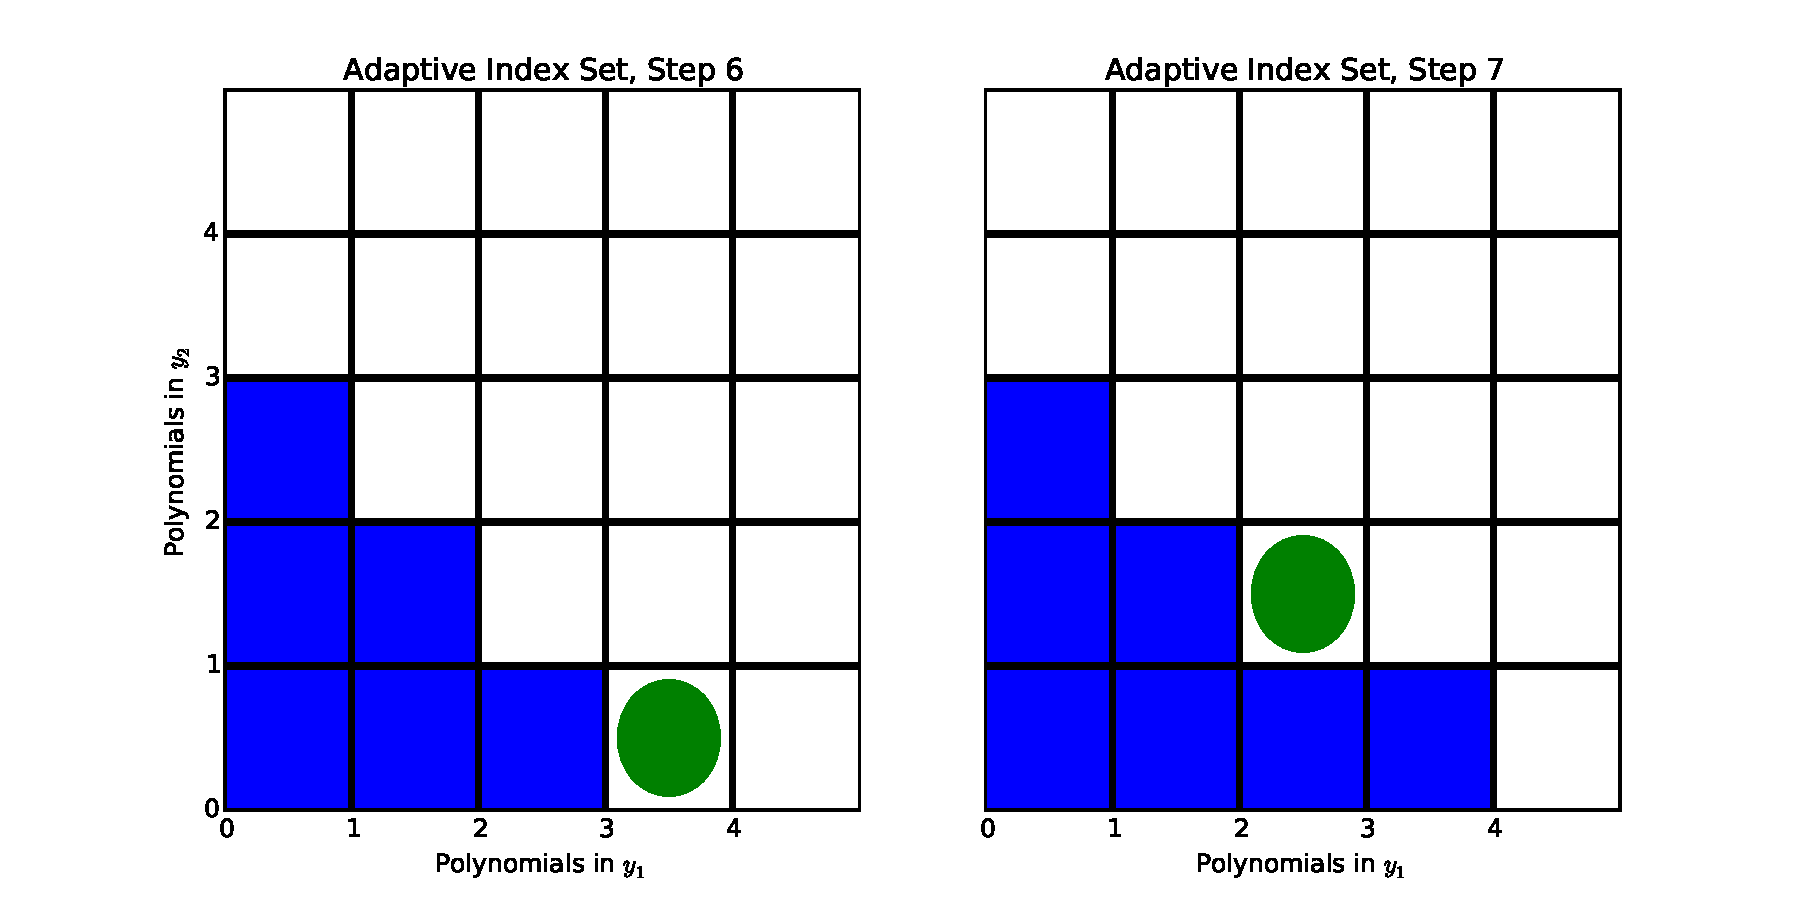
\includegraphics[width=\linewidth]{asc_step}
  \caption{Adaptive Sparse Grid Step}
  \label{fig:asg step}
\end{figure}
\begin{figure}[H]
  \centering
  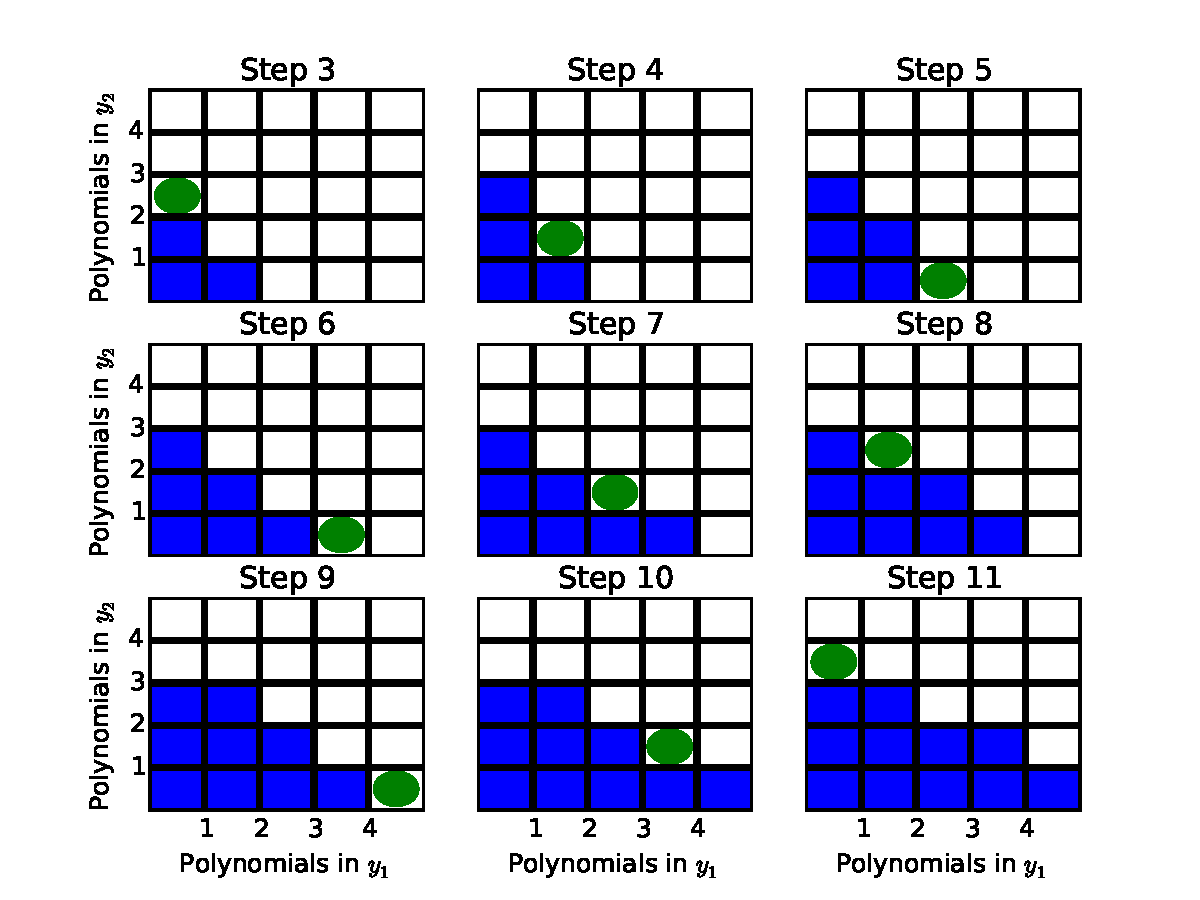
\includegraphics[width=0.7\linewidth]{asc_block}
  \caption{Adaptive Sparse Grid Progression}
  \label{fig:asg block}
\end{figure}

There are, however, some weak points in this algorithm.  First, the current algorithm has no predictive method
to determine the next polynomial index to include in the set; instead, it evaluates each potential index and
selects the one with the most impact \cite{Ayres}.  This is somewhat inefficient, because of SCgPC representations created
that are not used in the final product.  One improvement we make to this algorithm is to predict the impact of
un-evaluated polynomials based on the impact of predecessors.

In order to predict the most valuable polynomial to add to the expansion during an adaptive search, we first
identify a metric for value.  Because our interest is in second-order statistics, and the variance of the
polynomial expansions is the sum of the polynomial expansion coefficients, we consider the \emph{impact}
$\eta_k$ of a polynomial to be the square of its polynomial expansion coefficient,
\begin{equation}\label{eq: act poly impact}
  \eta_k = u_k^2.
\end{equation}
To estimate the impact of a polynomial whose coefficient is not yet calculated, we consider the average of the
preceeding polynomials.  That is, for a polynomial $k=(3,2,4)$ we average the impacts of $(2,2,4)$, $(3,1,4)$,
and $(3,1,3)$,
\begin{equation}\label{eq: poly impact}
  \tilde \eta_k = \frac{1}{N-j}\sum_{n=1}^N \eta_{k-e_n},
\end{equation}
where $\tilde \eta_k$ is the estimated impact of polynomial $k$, $e_n$ is a unit vector in dimension $n$, and
for every entry where $k-e_n$ would reduce one index to less than 0, it is skipped and $j$ is incremented by
one.  In this way any polynomial with some missing predecessors is still averaged appropriately with all
available information.  While occasionally this prediction algorithm may be misled, in general it saves
significantly over the previous algorithm.

Another weakness of the adaptive sparse grid algorithm is that 
there are certain types of models for which the adaptive algorithm will stall, converge too early, or
similarly fail.  For instance, if the partial derivative of the model with respect to any of the
input dimensions is zero when evaluated at the mean point (but nonzero elsewhere), the algorithm will falsely
converge prematurely, as adding additional polynomial orders to the input in question will not change the
value of the model at the mean point.  For example, consider a model
\begin{equation}
  f(a,b) = a^3b^3,
\end{equation}
with both $a$ and $b$ uniformly distributed on [-1,1].  We note the partial derivatives with respect to either
input variable evaluated at the central point (0,0) are zero.  The first polynomial index set point to
evaluate is zeroth-order in each dimension, [0,0].  We distinguish input domain points from polynomial index
set points by using parenthesis for the former and square brackets for the latter. The quadrature point to
evaluate this polynomial coefficient is (0,0), which, when evaluated, gives $f(0,0)=0$.  The next polynomial
index set combinations are [1,2] and [2,1].  For [1,2], the quadrature points required are
(0,$\pm\sqrt{1/3}$).  This evaluates to $f(0,\pm\sqrt{1/3})=0$, as well.  Because of symmetry, we obtain the
same result of [2,1].  According to our algorithm, because our old value was 0, and the sum of the new
contributions is 0, we have converged; however, we know this is false convergence.  While we expect few
applications for SCgPC to exhibit these zero partial derivatives in the input space, it is a limitation to be
aware of.  An argument can be made that, since lower-order polynomials correspond to lower-energy modes of the
modeled physics, it is expected that higher-order polynomials should rarely contribute to an accurate
expansion unless lower-order polynomials contribute as well.
 % 2
% Chapter Template

\chapter{Results for Stochastic Collocation for Generalized Polynomial Chaos} % Main chapter title

\label{ch:results scgpc} % Change X to a consecutive number; for referencing this chapter elsewhere, use \ref{ChapterX}

\lhead{Chapter 4. \emph{Results: SCgPC}} % Change X to a consecutive number; this is for the header on each page - perhaps a shortened title

%----------------------------------------------------------------------------------------
%	SECTION: INTRO
%----------------------------------------------------------------------------------------

\section{Introduction}\label{sec:res scgpc intro}
In this chapter we present results obtained using stochastic collocation for generalized polynomial chaos
expansions (SCgPC) using the three presented static polynomial sets (tensor product, hyperbolic cross, and
total degree) as well as the adaptive construction approach for polynomial sets.  We present performance on 
a variety of increasingly-complex
models, from linear polynomials to discontinuous products.  For each model, we demonstrate the
efficiency of each collocation method on a variety of input space sizes where possible.  The increasingly
complex models in addition to the increasing input space sizes will provide a survey of where
collocation-based methods clearly outperform Monte Carlo (MC) and where they fall short.

We use these six analytic models as a means to study convergence on the first two statistical moments of the
response.  This requires a high-precision evaluation of the moments, which is not practical for non-analytic
models.  We are concerned chiefly with the convergence rate of each model; that is, for the cost of increasing
the number of computation solves, how much error can be reduced.  Because Monte Carlo converges linearly on a
log-log plot of error versus solves, this linear convergence provides the benchmark for collocation methods.

Our primary objective in expanding the usability of collocation-based methods is to reduce the number of
computational model solves necessary to obtain reasonable second-order statistics for the model.  For each
analytic model, we present \emph{value figures} and \emph{convergence figures}.  

Value figures show the values of the mean or standard deviation obtained, along with the benchmark analytic
value as a dotted line.  MC performance is taken at a few representative points.  Error bars are provided
for MC and are estimated using the population variance,
\begin{equation}
  \epsilon_{95} = \frac{2\bar\sigma_M}{\sqrt{M}},
\end{equation}
\begin{equation}
  \bar\sigma_M^2 = \frac{M}{M-1}\sigma^2_M = \frac{M}{M-1}\qty(\frac{1}{M}\sum_{m=1}^M u(Y(\omega_m))^2 - \bar
  u(Y)^2_N),
\end{equation}
where $Y(\omega_m)$ are a set of $M$ independent realizations taken from the identically-distributed input space.
These error bars estimate where the value of the statistic is with a probability of at least 0.75, as discussed in
section \ref{sec:stat moments}.  The estimate of
this error improves as additional samples are taken.

Convergence figures are
log-log error graphs with the number of computational solves required on the x-axis and error with respect to the analytic
solution on the y-axis.  The distinct series plotted demonstrate results obtained for each UQ method.  
The series we show here are analog traditional MC; static 
SCgPC expansions using the hyperbolic
cross index set (SC:HC), total degree index set (SC:TD), and (where possible) tensor product index set (SC:TP); 
and adaptive SCgPC (SC:adapt).
Each
series obtains additional values by increasing the refinement of the method.  For MC, additional
random samples are added.  For static SCgPC, higher-order polynomials are used in the representative expansion.  For
adaptive methods, additional solves are allowed to adaptively include additional polynomials.

The measure of success for a method is not dependent on the absolute value of the error shown.  While
informative, we are more concerned with how increasing refinement reduces error.  The
rate of convergence as refinement increases determines the desirability of the method for that model.  We
expect the rate of convergence to depend primarily two factors: the dimensionality of the uncertain space for the
model, and the continuity or smoothness of the response measured.  The value of the error, on the other hand, will additionally
depend on how well a particular choice of polynomials matches the analytic polynomial representation of the model.
We consider the convergence of both the mean and the standard deviation for each model.

The uncertainty quantification analysis in this chapter is all performed in \raven{} \cite{raven} on external python
models.  Results from \raven{} computations were written to file using 10 digits of accuracy.
As a result, any apparent convergence past this level of accuracy is coincidental or the result of
machine-exact values, and we consider a relative difference of $10^{-10}$ to be converged.




\section{Tensor Monomials}
\subsection{Description}\label{mod:tensor monom}
The simplest model we make use of is a first-order tensor polynomial (tensor monomial) combination \cite{Ayres}.
Each term in this polynomial expression is at most linear in any dimension.  This provides a simple calculation
of the statistical moments, and no second-order polynomials are required to exactly reproduce this model.
The mathematical expression for tensor monomials is
\begin{equation}
  u(Y) = \prod_{n=1}^N (y_n+1).
\end{equation}
For example, for $N=3$ we have
\begin{equation}
  u(Y) = y_1y_2y_3 + y_1y_2 + y_1y_3 + y_2y_3 + y_1 + y_2 + y_3 + 1.
\end{equation}
For this model we can distribute the uncertain inputs in several ways because of its simplicity: uniformly on [-1,1], uniformly on
[0,1], and normally on [$\mu,\sigma$]. A summary of analytic statistics is given in Table \ref{tab:tensormono moments}.
The two-dimensional representation of this response is given in Figure \ref{fig: tensor monomials}.
\begin{figure}[htb]
  \centering
  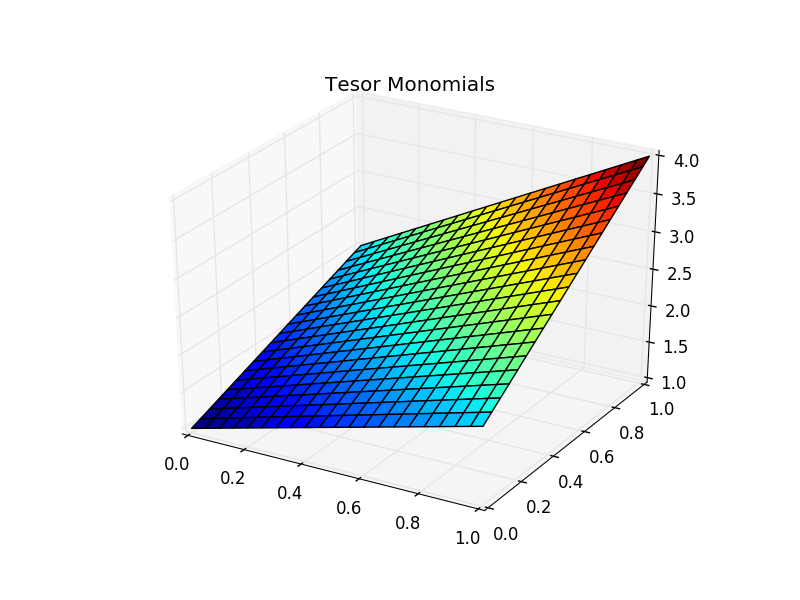
\includegraphics[width=0.7\linewidth]{anlmodels/tensor_monom}
  \caption{Tensor Monomials Response}
  \label{fig: tensor monomials}
\end{figure}

\begin{table}[H]
  \centering
  \begin{tabular}{c|c|c}
    Distribution & Mean & Variance \\\hline
    $\mathcal{U}[-1,1]$ & 1 & $\qty(\frac{4}{3})^N - 1$ \\
    $\mathcal{U}[0,1]$ & $\qty(\frac{3}{4})^N$ & $\qty(\frac{7}{3})^N - \qty(\frac{3}{4})^{2N}$ \\
    $\mathcal{N}[\mu,\sigma]$ & $\prod_{n=1}^N (\mu_{y_n}+1)$ & $\prod_{n=1}^N[(\mu_{y_n}+1)^2+\sigma_{y_n}^2]
    - \prod_{n=1}^N (\mu_{y_n}+1)^2$
  \end{tabular}
  \caption{Analytic Expressions for Tensor Monomial Case}
  \label{tab:tensormono moments}
\end{table}
For purposes of demonstration, we pick several increasing orders of dimensionality: three input variables, five variables, and
ten variables.

\subsection{Discussion}
As this polynomial contains only combinations of
first-order polynomials, we expect the Tensor Product index set construction method to be very efficient
in absolute error.  
As such, it will be difficult to observe the convergence rate for this method, as it converges exactly with 
first-order polynomials.
Because the model has infinite continuity, we expect all collocation-based
methods to be quite efficient.  Plots with the values and errors of the mean and standard deviation are given
for each of three (Figures \ref{fig:tensormono mean values 3} through \ref{fig:tensormono var errors 3}),
five (Figures \ref{fig:tensormono mean values 5} through \ref{fig:tensormono var errors 5}), 
and ten (Figures \ref{fig:tensormono mean values 10} through \ref{fig:tensormono var errors 10})
input parameters.  Note especially that TP exactly reproduces the original model with expansion order 1, so no convergence is
observed past the initial sampling point.

\subsection{Tensor Monomials: 3 Inputs}
The strength of collocation methods is clear for this small-dimensionality problem of three uncertain inputs.
The convergence on the
mean and standard deviation is swift for all the methods.  The convergence of the mean is instant for all methods, since
the linear nature of the problem means only the zeroth-order polynomial term is required to exactly reproduce the mean.
More convergence behavior can be seen for the standard deviation.
Because hyperbolic cross polynomials emphasize single-variable polynomials over cross terms, it is the slowest to reach
effectively zero error.  Similarly, the total degree quickly obtains most of the polynomials in the exact expansion,
but takes a few levels to include the term that has all the input variables in it.  Because first-order tensor product
polynomials is exactly the model itself, it converges instantly.
The adaptive SCgPC method initially explores high-order polynomials before finding the remaining tensor
monomials, which makes it less directly efficient than tensor product but otherwise desirable over the other
two static polynomial sets.
\begin{figure}[H]
  \centering
  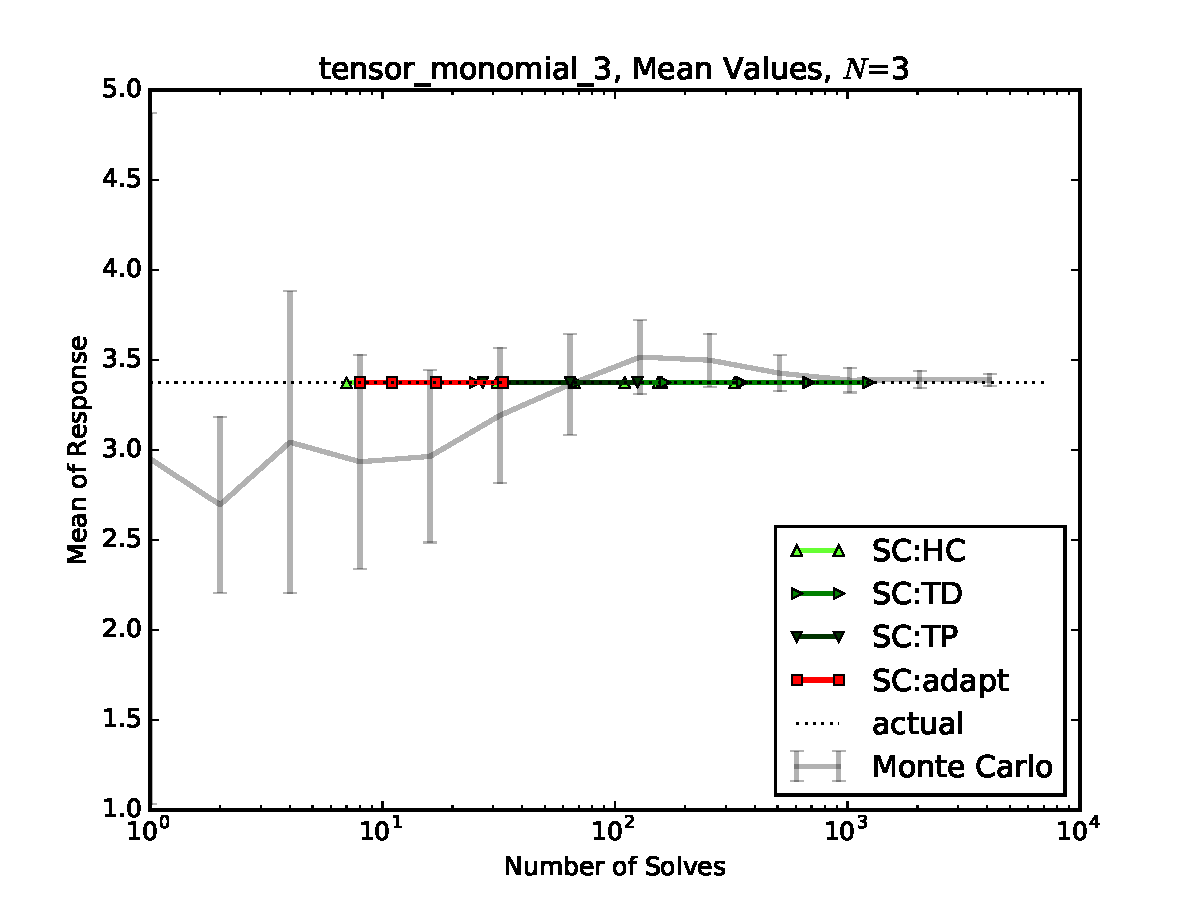
\includegraphics[width=0.7\linewidth]{anlmodels/tensor_monomial_3_mean_vals_nohdmr}
  \caption{Tensor Monomial, $N=3$, Mean Values}
  \label{fig:tensormono mean values 3}
\end{figure}
\begin{figure}[H]
  \centering
  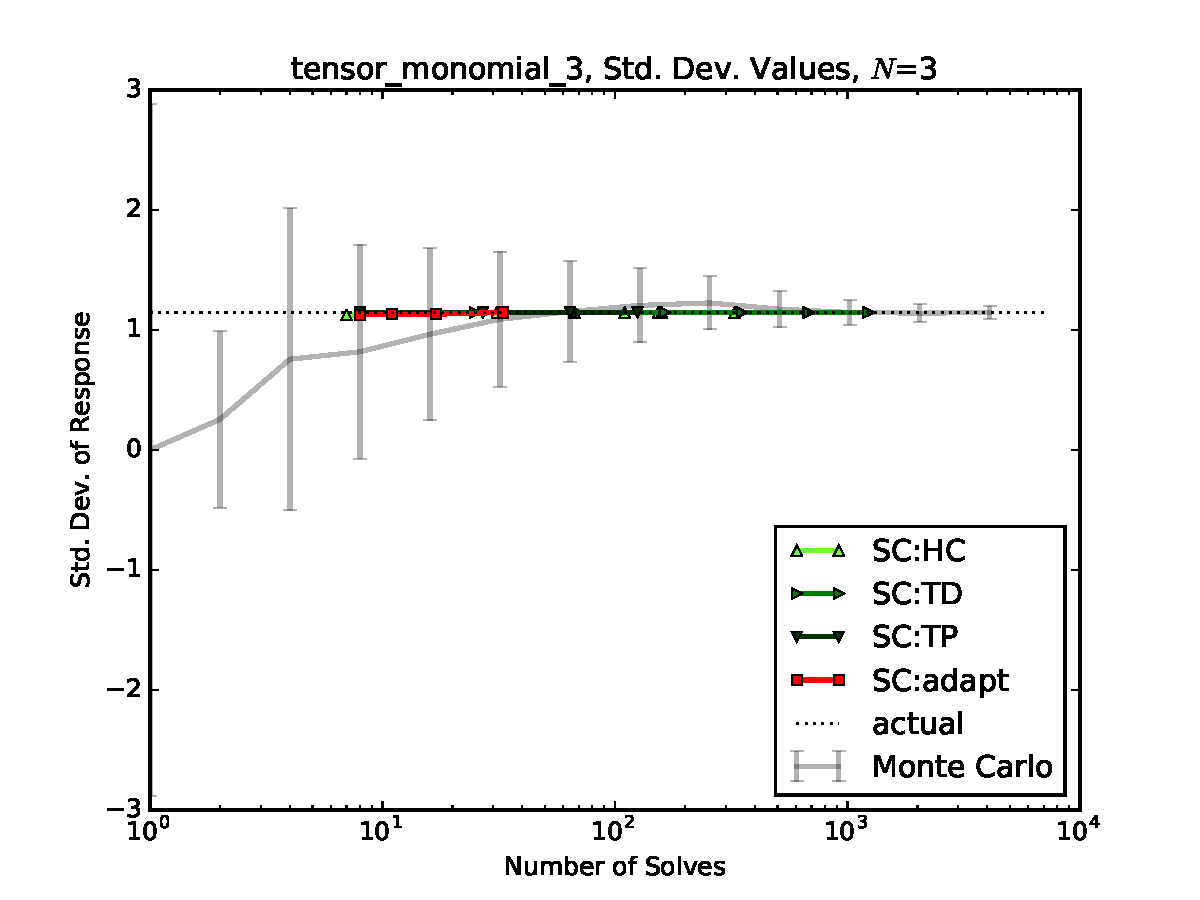
\includegraphics[width=0.7\linewidth]{anlmodels/tensor_monomial_3_var_vals_nohdmr}
  \caption{Tensor Monomial, $N=3$, Std. Dev. Values}
  \label{fig:tensormono var values 3}
\end{figure}

\begin{figure}[H]
  \centering
  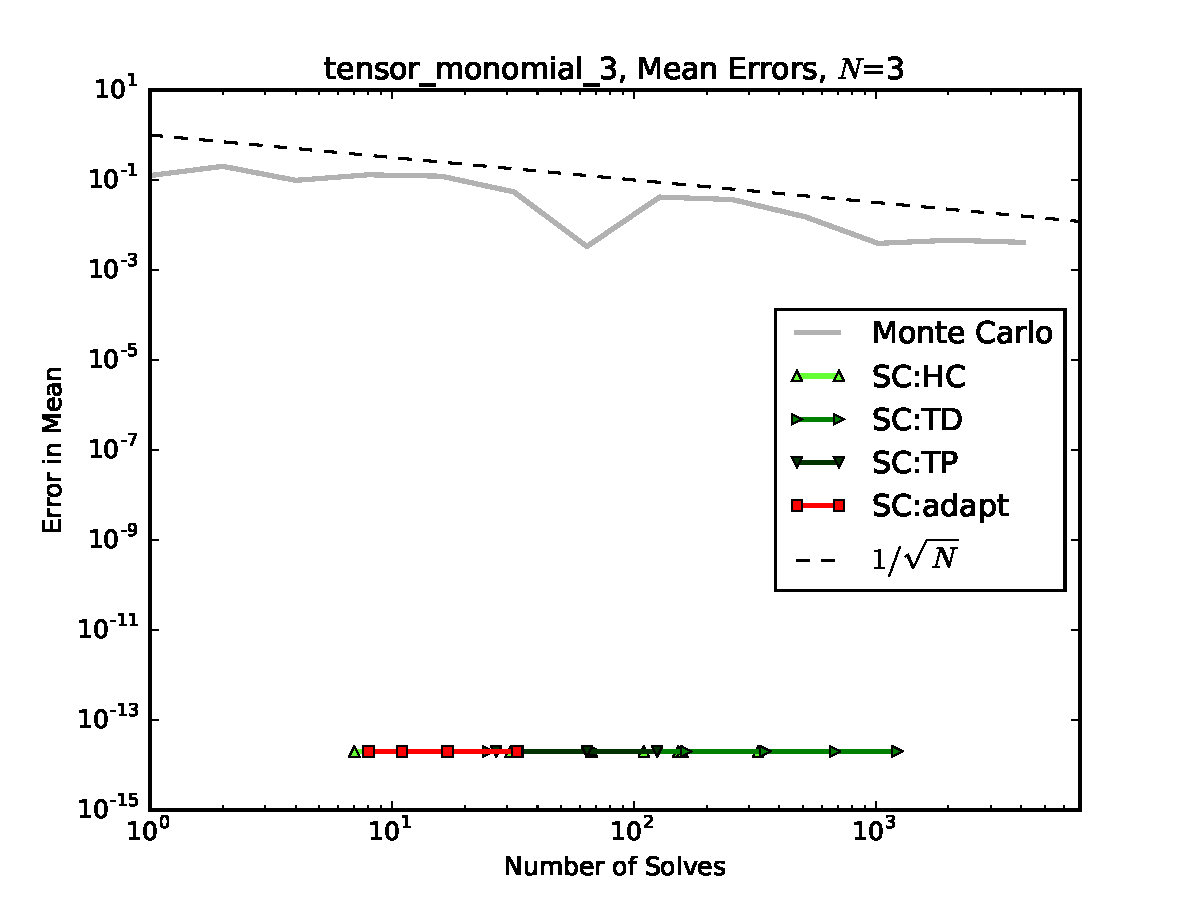
\includegraphics[width=0.7\linewidth]{anlmodels/tensor_monomial_3_mean_errs_nohdmr}
  \caption{Tensor Monomial, $N=3$, Mean Convergence}
  \label{fig:tensormono mean errors 3}
\end{figure}
\begin{figure}[H]
  \centering
  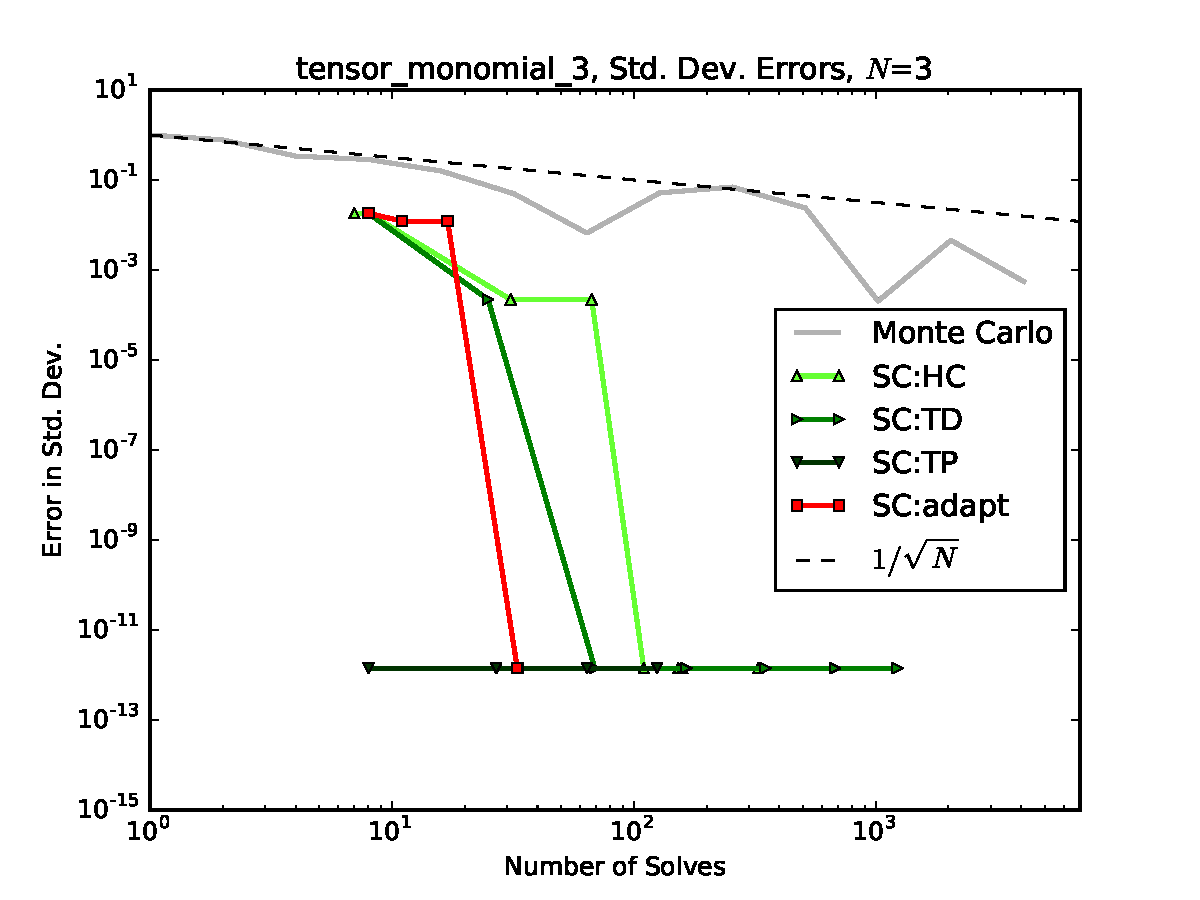
\includegraphics[width=0.7\linewidth]{anlmodels/tensor_monomial_3_variance_errs_nohdmr}
  \caption{Tensor Monomial, $N=3$, Std. Dev. Convergence}
  \label{fig:tensormono var errors 3}
\end{figure}

\subsection{Tensor Monomials: 5 Inputs}
While the convergence on the mean is still direct for the five-dimensional input problem, we begin to see
degradation in the convergence on the standard deviation for collocation-based methods.  
As with the three variable case, the mean is trivial and obtained with the zeroth-order polynomial.  
Exponential
convergence can be seen for the total degree and hyperbolic cross polynomials, while the adaptive
method
is still exploring higher-order polynomials as more likely candidates for inclusion in the expansion and hasn't
seen the same rapid convergence curve yet.  This is a flaw in the default search parameters for the adaptive
algorithm when applied to this model.
Total Degree outperforms Hyperbolic Cross and Adaptive, as
the adaptive search algorithm struggles to find the optimal tensors of low-order polynomials required.  Hyperbolic
Cross is outperformed by Total Degree as expected for a problem with this level of regularity.
\begin{figure}[H]
  \centering
  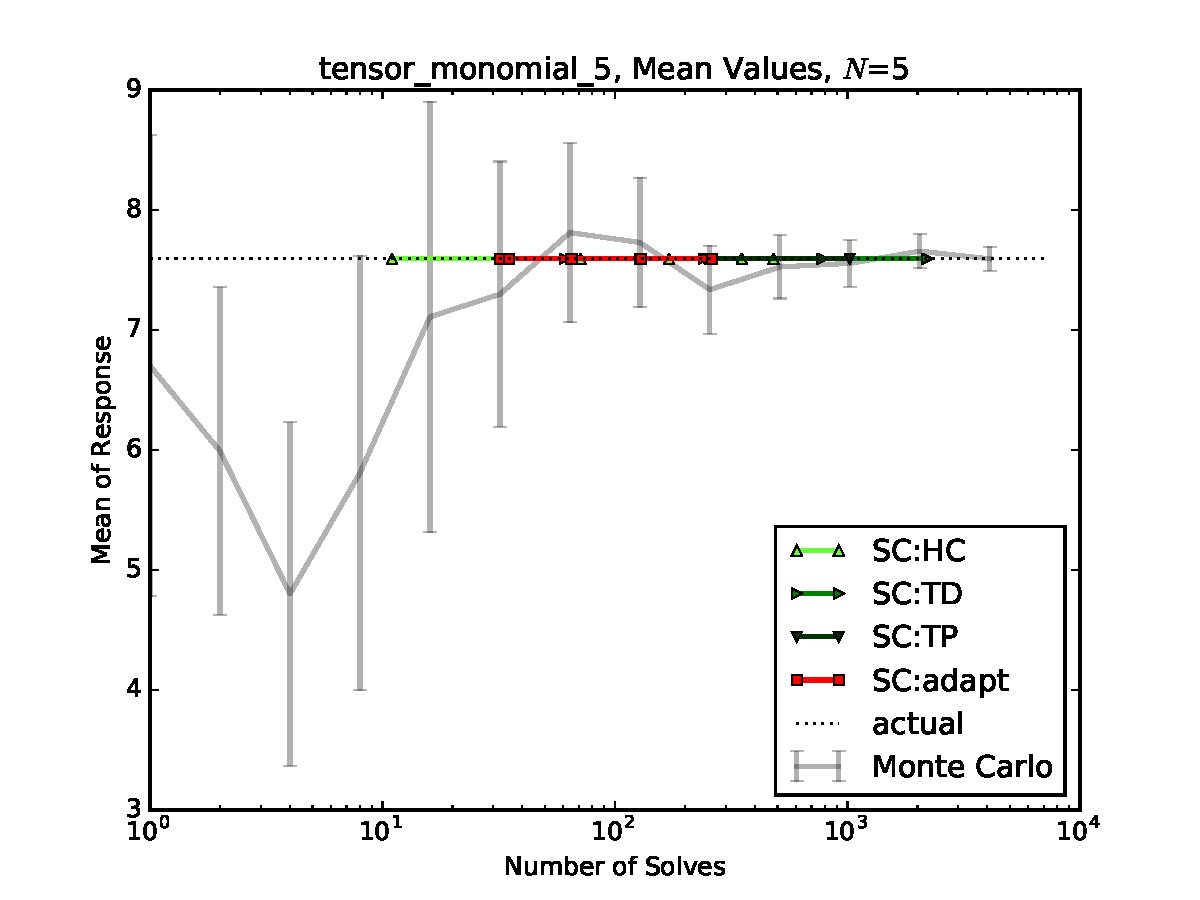
\includegraphics[width=0.7\linewidth]{anlmodels/tensor_monomial_5_mean_vals_nohdmr}
  \caption{Tensor Monomial, $N=5$, Mean Values}
  \label{fig:tensormono mean values 5}
\end{figure}
\begin{figure}[H]
  \centering
  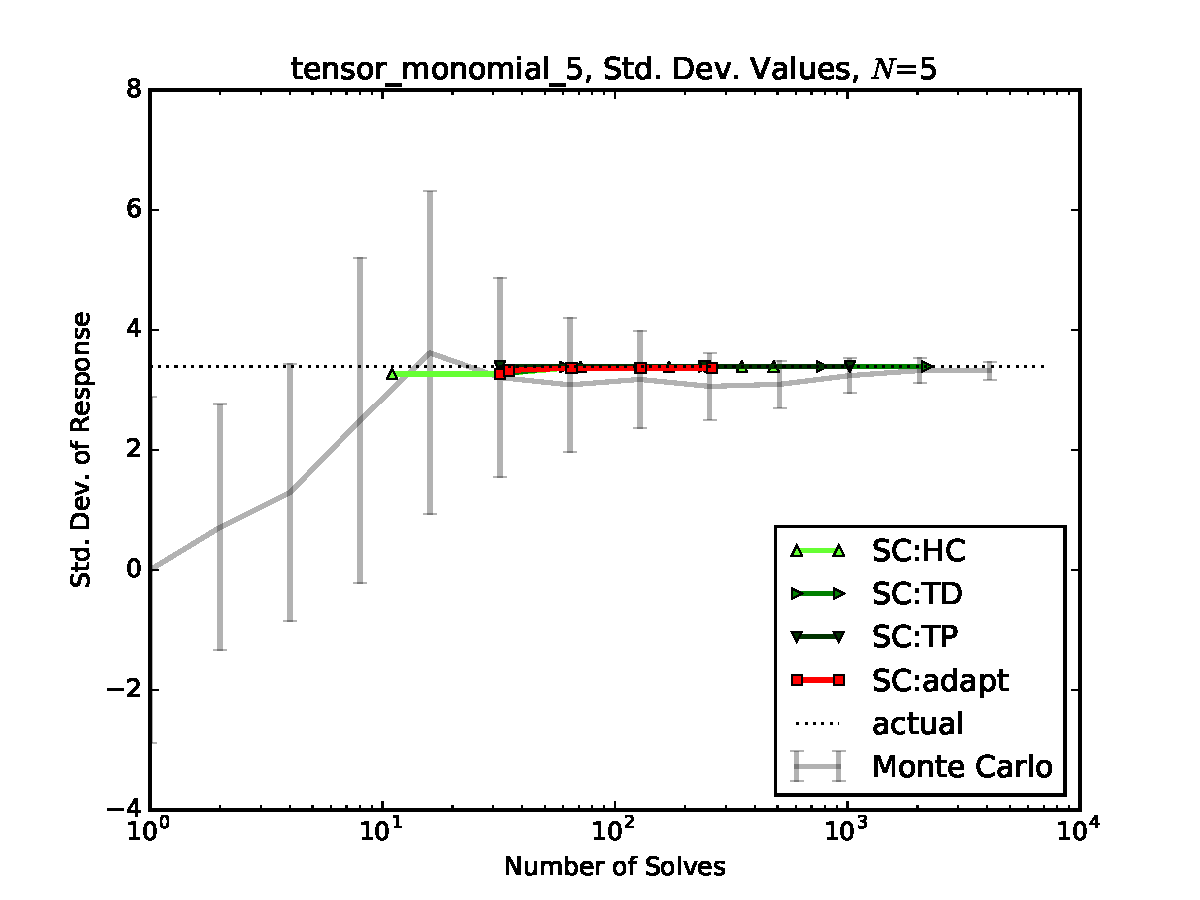
\includegraphics[width=0.7\linewidth]{anlmodels/tensor_monomial_5_var_vals_nohdmr}
  \caption{Tensor Monomial, $N=5$, Std. Dev. Values}
  \label{fig:tensormono var values 5}
\end{figure}

\begin{figure}[H]
  \centering
  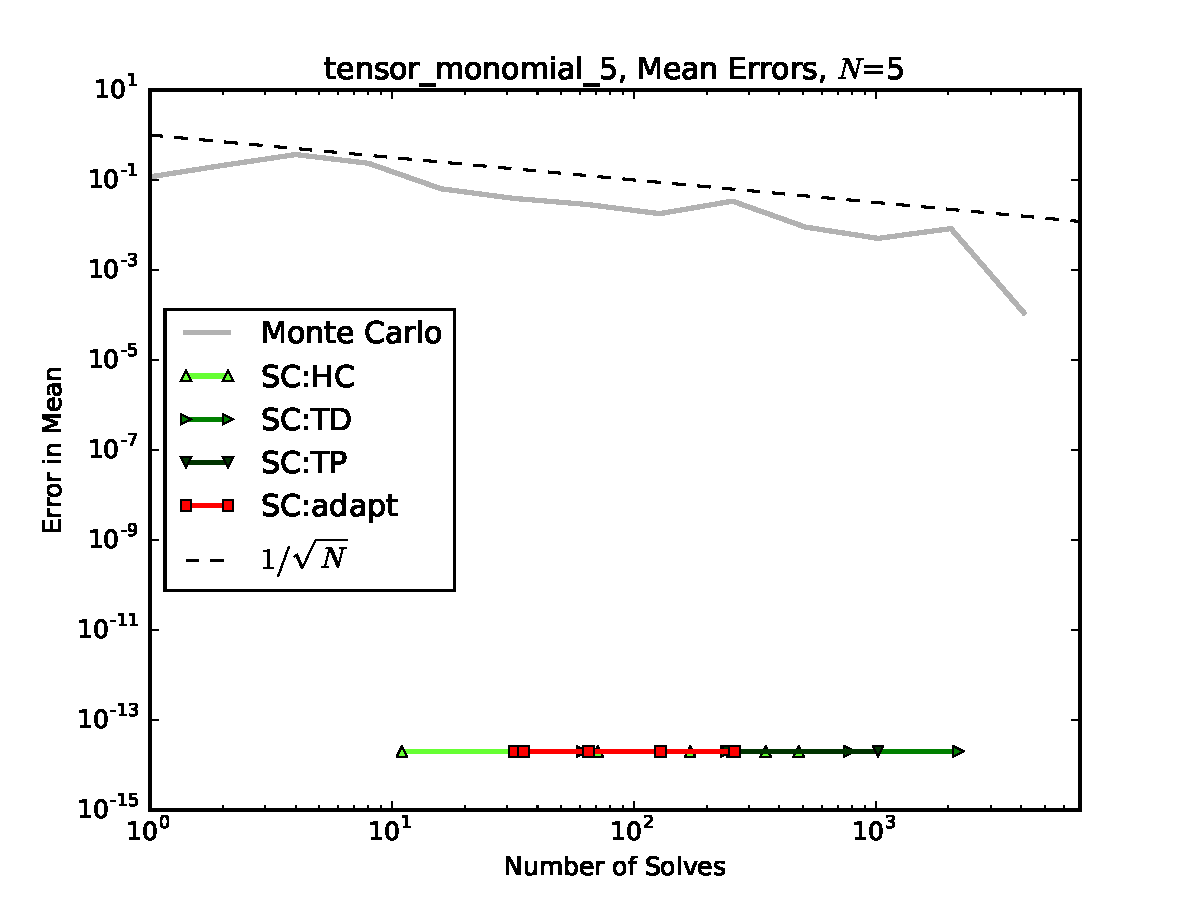
\includegraphics[width=0.7\linewidth]{anlmodels/tensor_monomial_5_mean_errs_nohdmr}
  \caption{Tensor Monomial, $N=5$, Mean Convergence}
  \label{fig:tensormono mean errors 5}
\end{figure}
\begin{figure}[H]
  \centering
  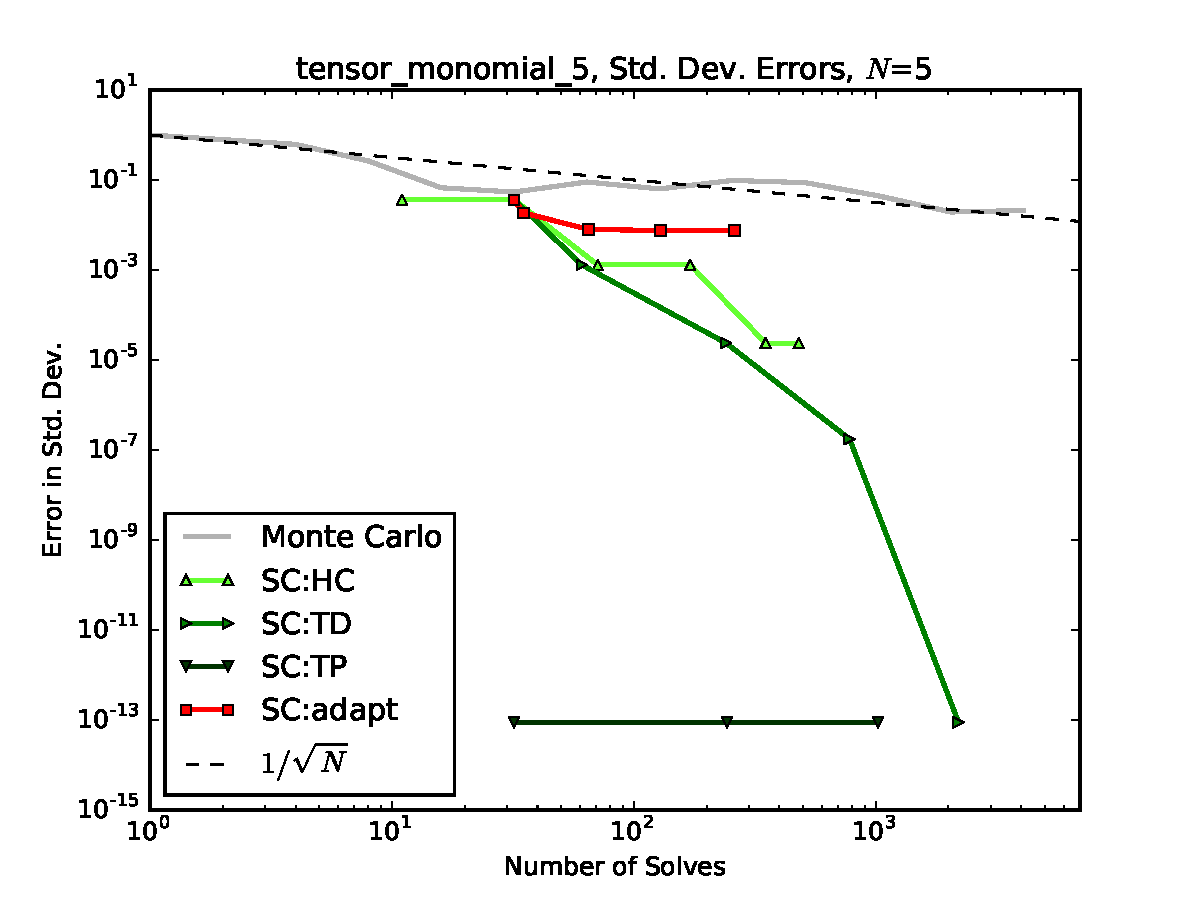
\includegraphics[width=0.7\linewidth]{anlmodels/tensor_monomial_5_variance_errs_nohdmr}
  \caption{Tensor Monomial, $N=5$, Std. Dev. Convergence}
  \label{fig:tensormono var errors 5}
\end{figure}

\subsection{Tensor Monomials: 10 Inputs}
As we increase to ten inputs, we see significant degradation of all the collocation methods in converging on
the standard deviation.  While it appears there might be exponential convergence, the curvature is quite large, and
only somewhat better than linear convergence is observed for up to 1000 computational solves.  One reason the
adaptive method does not perform more admirably for this case is the equal-weight importance of all the input
terms as well as the polynomial terms; the high-dimensional space takes considerable numbers of runs to
explore thoroughly, and this model contains some of the most difficult polynomials to find adaptively: those including
all ten of the inputs. 
\begin{figure}[H]
  \centering
  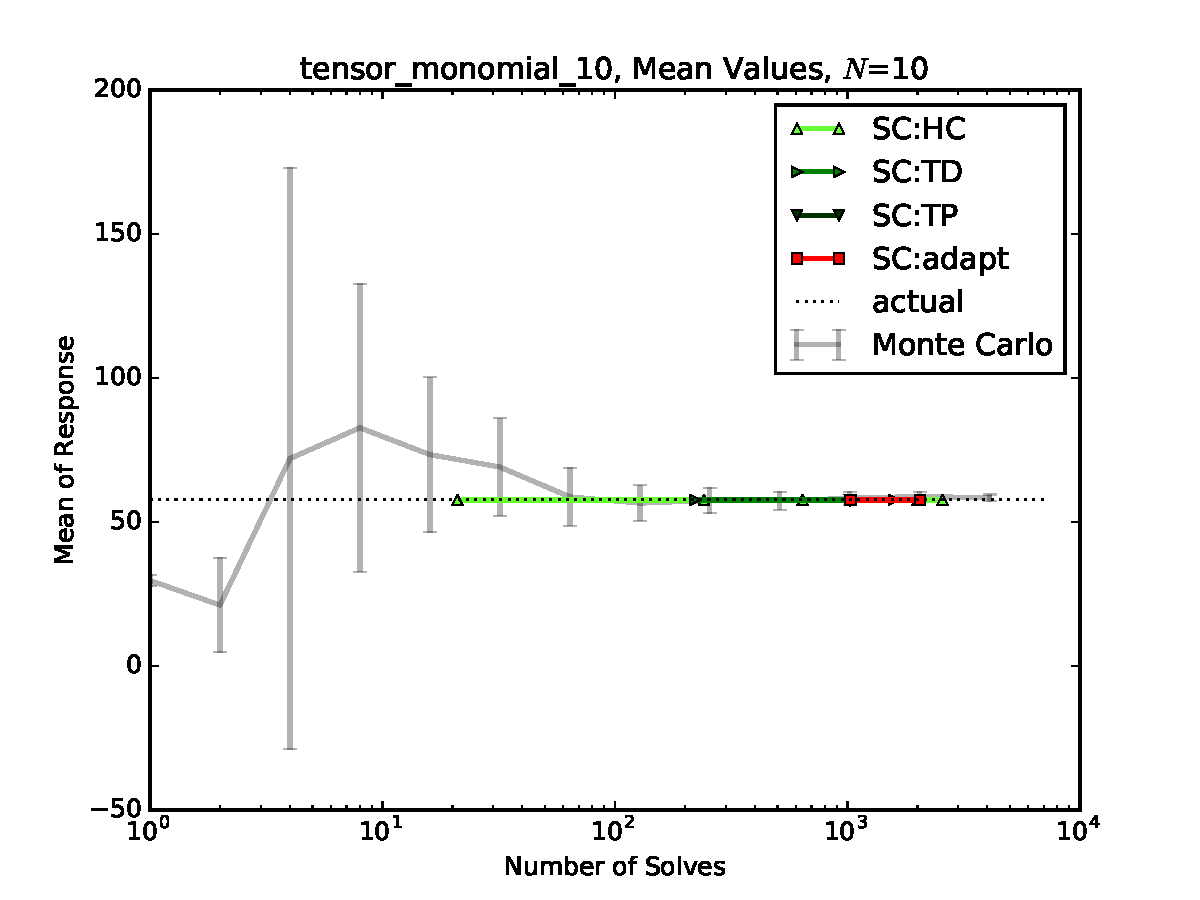
\includegraphics[width=0.7\linewidth]{anlmodels/tensor_monomial_10_mean_vals_nohdmr}
  \caption{Tensor Monomial, $N=10$, Mean Values}
  \label{fig:tensormono mean values 10}
\end{figure}
\begin{figure}[H]
  \centering
  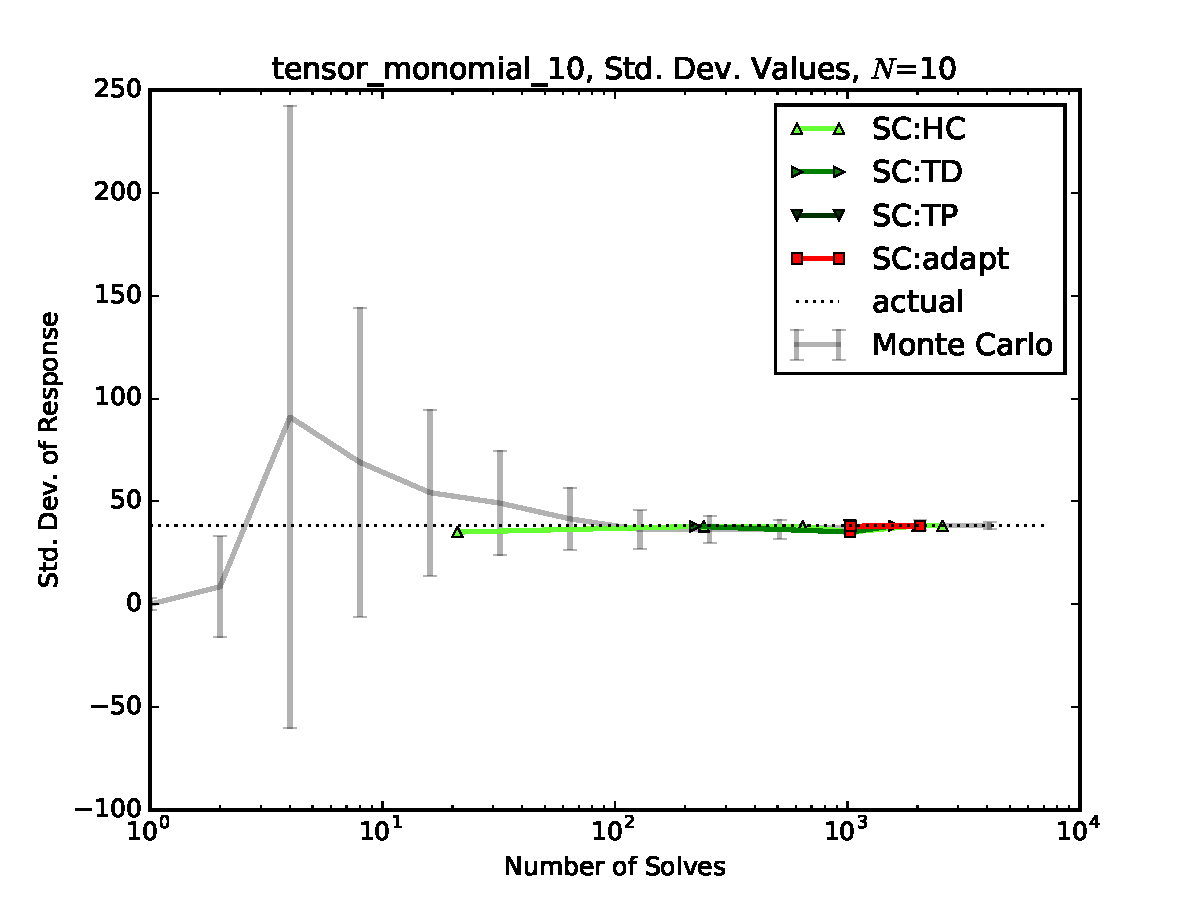
\includegraphics[width=0.7\linewidth]{anlmodels/tensor_monomial_10_var_vals_nohdmr}
  \caption{Tensor Monomial, $N=10$, Std. Dev. Values}
  \label{fig:tensormono var values 10}
\end{figure}

\begin{figure}[H]
  \centering
  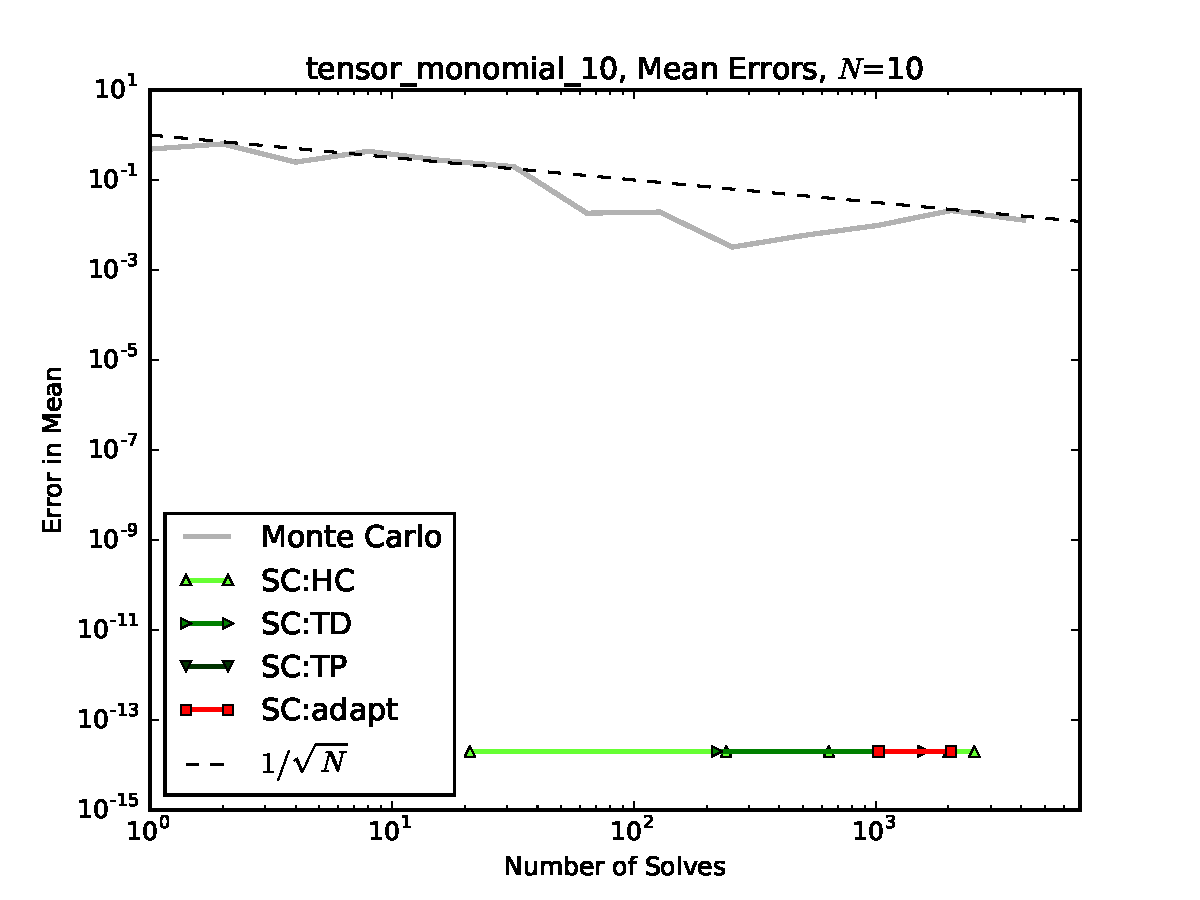
\includegraphics[width=0.7\linewidth]{anlmodels/tensor_monomial_10_mean_errs_nohdmr}
  \caption{Tensor Monomial, $N=10$, Mean Convergence}
  \label{fig:tensormono mean errors 10}
\end{figure}
\begin{figure}[H]
  \centering
  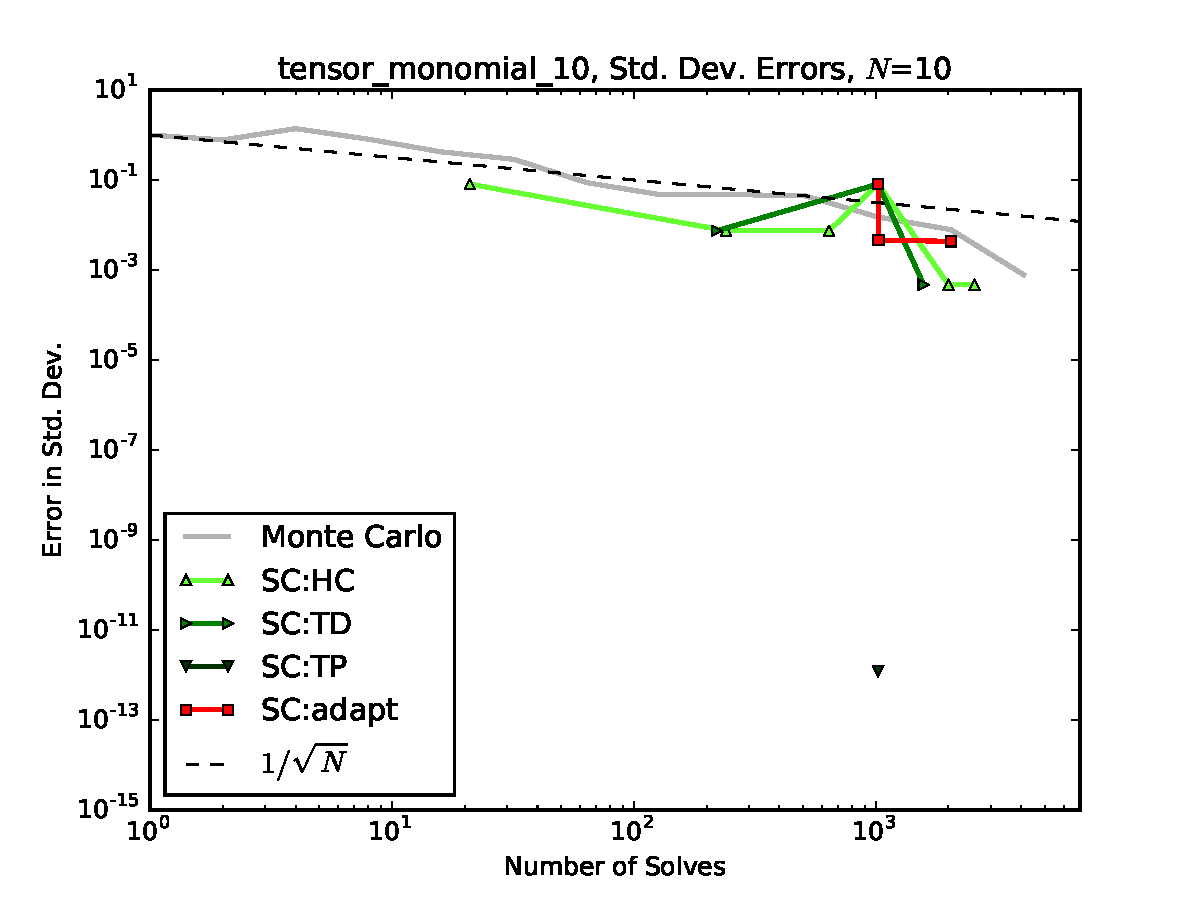
\includegraphics[width=0.7\linewidth]{anlmodels/tensor_monomial_10_variance_errs_nohdmr}
  \caption{Tensor Monomial, $N=10$, Std. Dev. Convergence}
  \label{fig:tensormono var errors 10}
\end{figure}


\section{Sudret Polynomial}
\subsection{Description}\label{mod:sudret}
The polynomial used by Sudret in his work \cite{sudret} is another tensor-like polynomial, and is a test case traditionally used to
identify convergence on sensitivity parameters.  It is similar to tensor monomials because it is constructed by the tensor
product of simple polynomials; in this case, Sudret used second-order polynomials.  As a result, only zeroth or second-order
polynomials exist in the expression.  Statistical moments are also quite straightforward for this model.
The mathematical expression for Sudret polynomials is
\begin{equation}
  u(Y) = \frac{1}{2^N}\prod_{n=1}^N (3y_n^2+1).
\end{equation}
The two-dimensional representation of this response is given in Figure \ref{fig: sudret}.
\begin{figure}[htb]
  \centering
  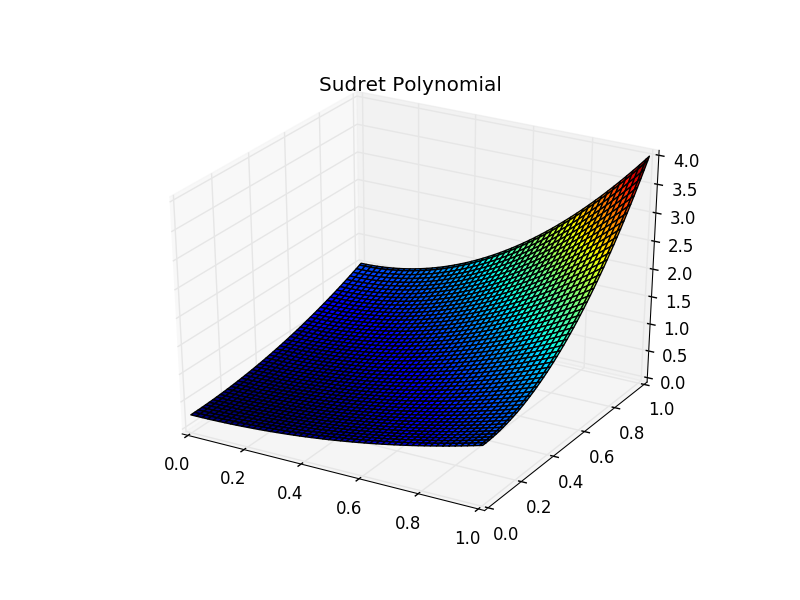
\includegraphics[width=0.7\linewidth]{anlmodels/sudret}
  \caption{Sudret Polynomial Response}
  \label{fig: sudret}
\end{figure}
The variables are distributed uniformly on [0,1].

The statistical moments and sensitivities for this model are given in
Table \ref{tab:sudret}, where $\mathcal{S}_n$ is the global Sobol sensitivity of $u(Y)$ to perturbations in
$y_n$.

\begin{table}[H]
  \centering
  \begin{tabular}{c c}
    Statistic & Expression \\\hline
    Mean & 1 \\
    Variance & $\qty(\frac{6}{5})^N - 1$ \\
    $\mathcal{S}_n$ & $\frac{5^{-n}}{(6/5)^N-1}$
  \end{tabular}
  \caption{Analytic Expressions for Sudret Case}
  \label{tab:sudret}
\end{table}
Because of its similarity to tensor polynomials, the cases we show are three inputs and five inputs.

\subsection{Discussion}
The Sudret polynomial model is a near neighbor to the
tensor monomials model; however, it includes only even-ordered polynomials.
Because the model is still a tensor product, the tensor product collocation method 
converges most directly in all dimensionality cases.

An interesting feature of the mean for
this model is that the zeroth-order expansions tend to estimate the variance more accurately than the
first-order expansions; as a result, it appears that the error is very small then grows rapidly.  This is
misleading to considering convergence, however, as the initial approximation exhibits some cancellation of
errors to obtain such an ``accurate'' result.

\subsection{Sudret Polynomial: 3 Inputs}
As with the tensor monomials, we see a good rate of convergence for many of the polynomial methods.  With
this model, the mean is not trivially given by the zeroth-order polynomial, and so some convergence is seen
in obtaining the expected value.  The total degree and adaptive methods converge at a similar rate for
the mean, while the hyperbolic cross demonstrates its poor convergence for highly regular systems with
nonlinear cross-term effects.  Quickest to converge (aside from the tensor product case) is the adaptive
SCgPC, because its search method allows it to discover the second-order polynomials quickly.

Similar behavior is seen for the standard deviation.
The tensor product still converges very rapidly, and total degree shows a good rate of convergence, while
hyperbolic cross demonstrates poor convergence.
\begin{figure}[H]
  \centering
  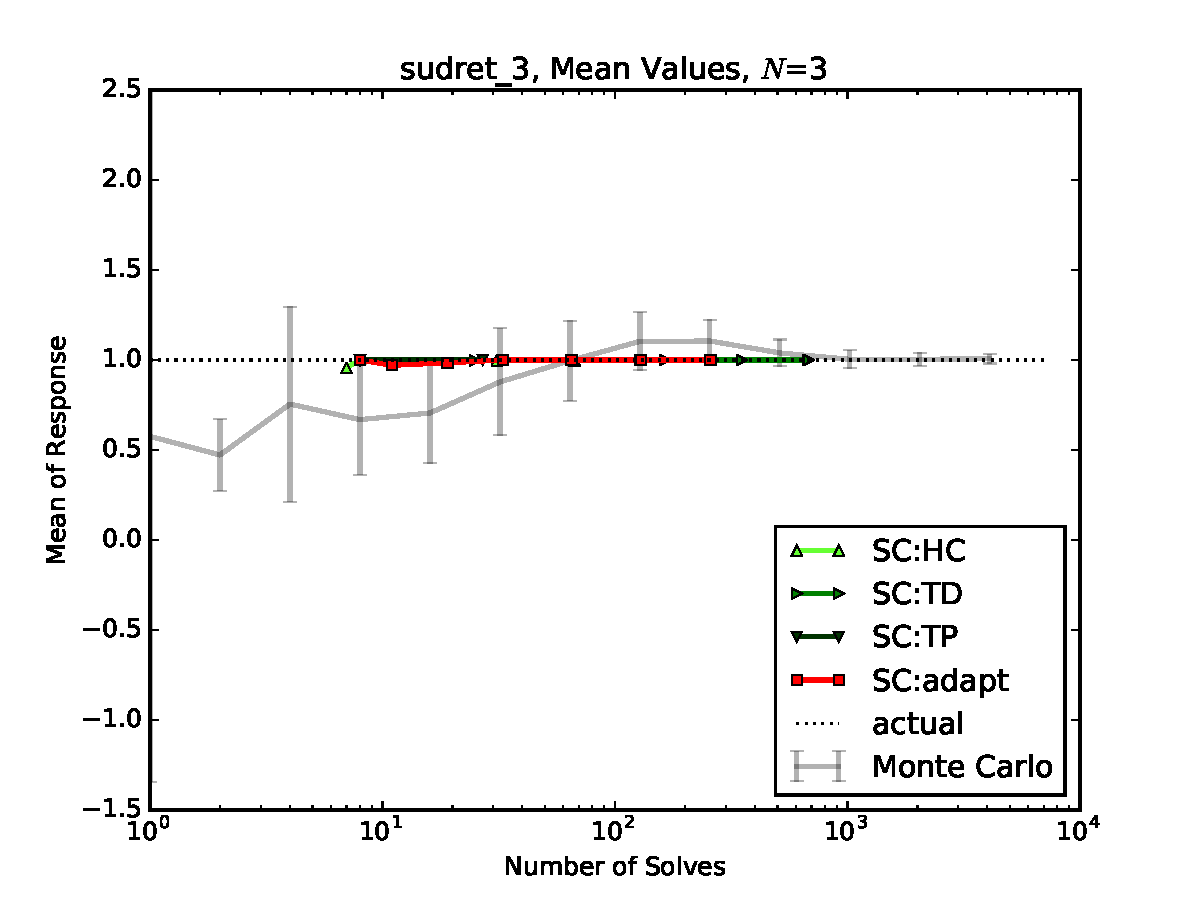
\includegraphics[width=0.7\linewidth]{anlmodels/sudret_3_mean_vals_nohdmr}
  \caption{Sudret Polynomial, $N=3$, Mean Values}
  \label{fig:sudretpoly mean values 3}
\end{figure}
\begin{figure}[H]
  \centering
  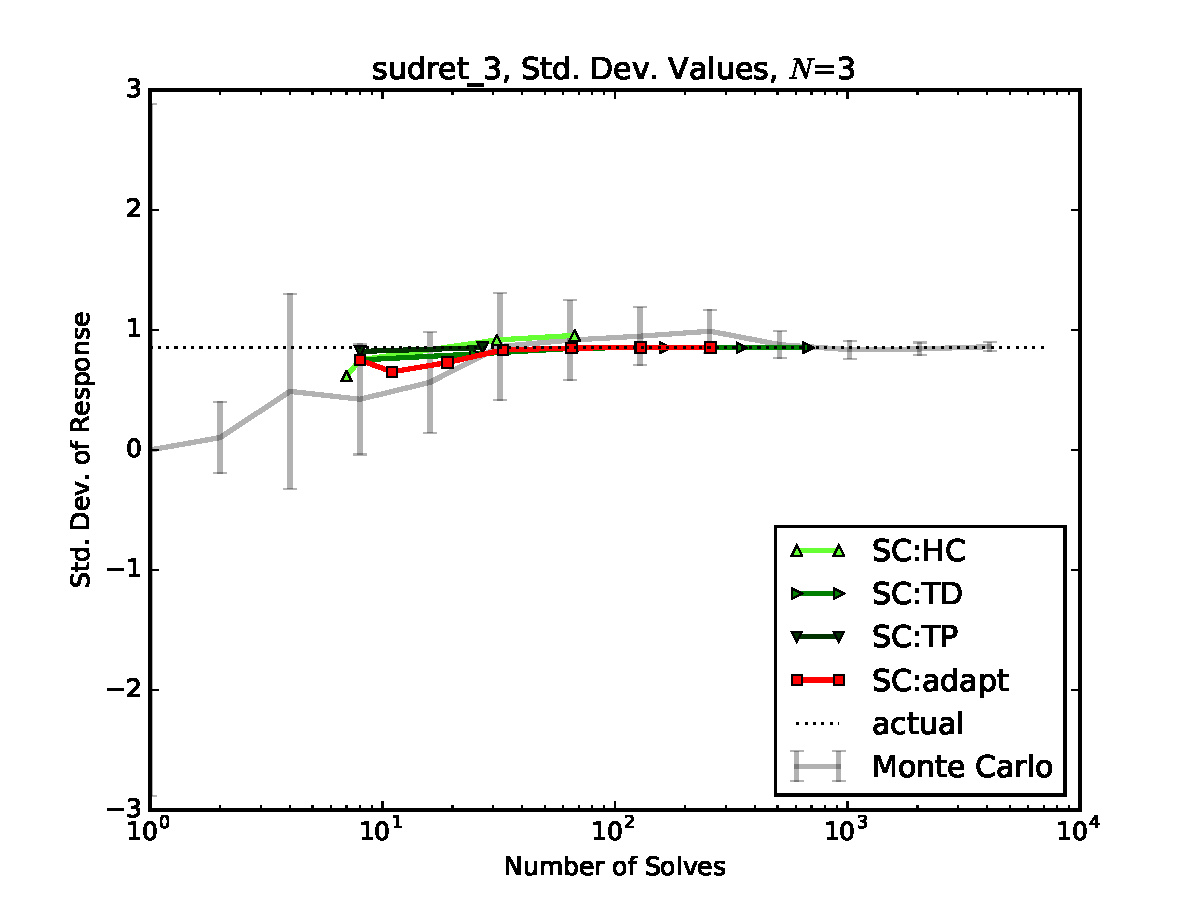
\includegraphics[width=0.7\linewidth]{anlmodels/sudret_3_var_vals_nohdmr}
  \caption{Sudret Polynomial, $N=3$, Std. Dev. Values}
  \label{fig:sudretpoly var values 3}
\end{figure}

\begin{figure}[H]
  \centering
  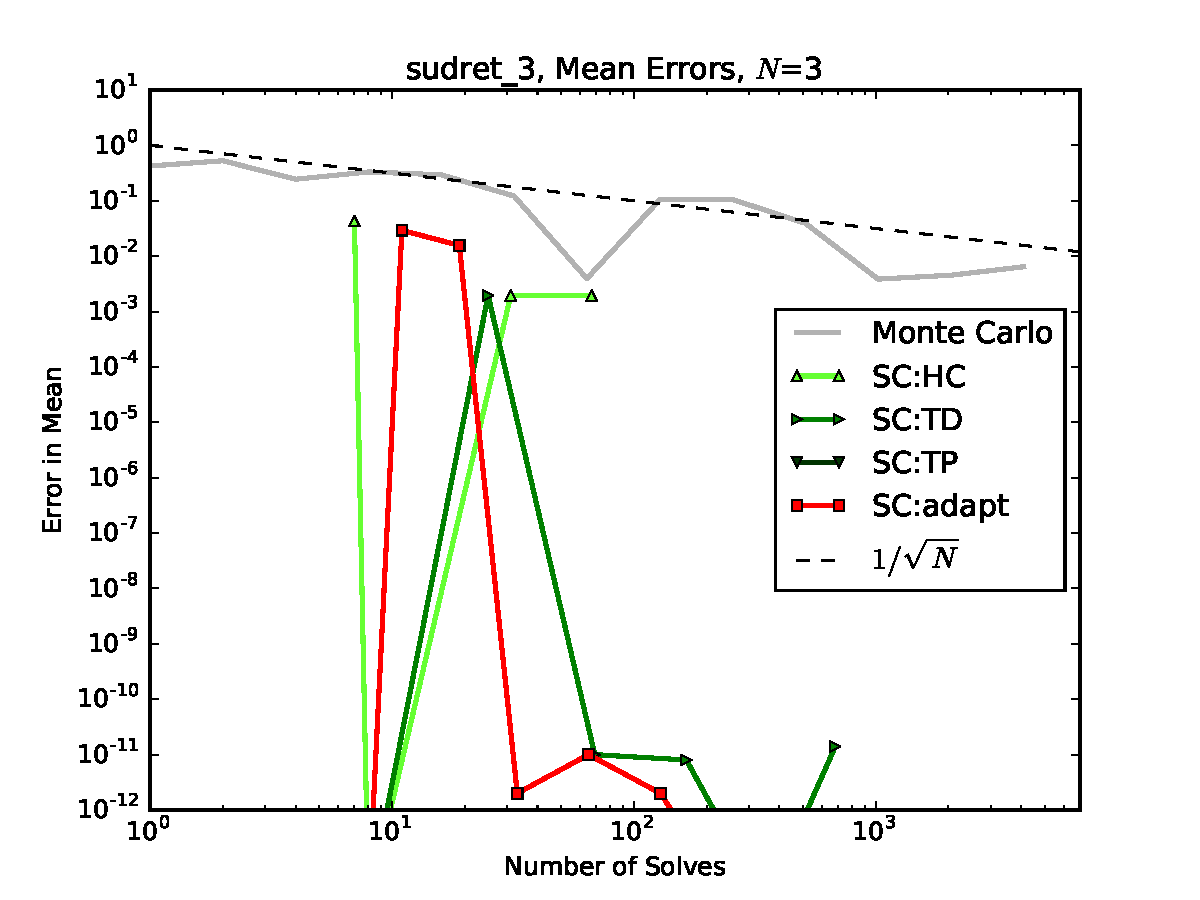
\includegraphics[width=0.7\linewidth]{anlmodels/sudret_3_mean_errs_nohdmr}
  \caption{Sudret Polynomial, $N=3$, Mean Convergence}
  \label{fig:sudretpoly mean errors 3}
\end{figure}
\begin{figure}[H]
  \centering
  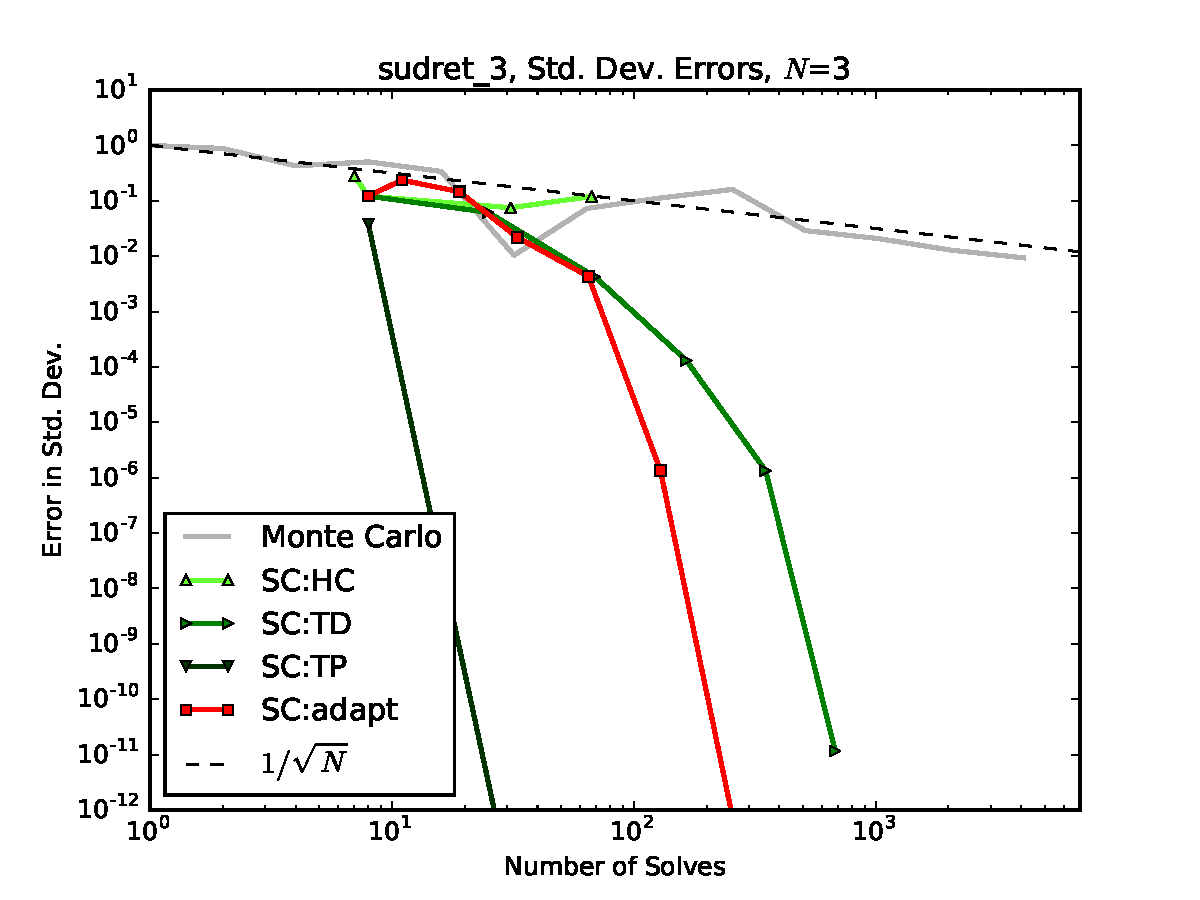
\includegraphics[width=0.7\linewidth]{anlmodels/sudret_3_variance_errs_nohdmr}
  \caption{Sudret Polynomial, $N=3$, Std. Dev. Convergence}
  \label{fig:sudretpoly var errors 3}
\end{figure}

\subsection{Sudret Polynomial: 5 Inputs}
In the five-input case for the Sudret polynomials, we see slower but strong convergence for adaptive and
total degree methods.
For the mean, each method is showing some level of exponential convergence, with the exception of the
hyperbolic cross method.  For the standard deviation,
however, the radius of curvature for the convergence is quite large.  This demonstrates the negative impact
growing input spaces have on the effectiveness of collocation methods in comparison with MC.
\begin{figure}[H]
  \centering
  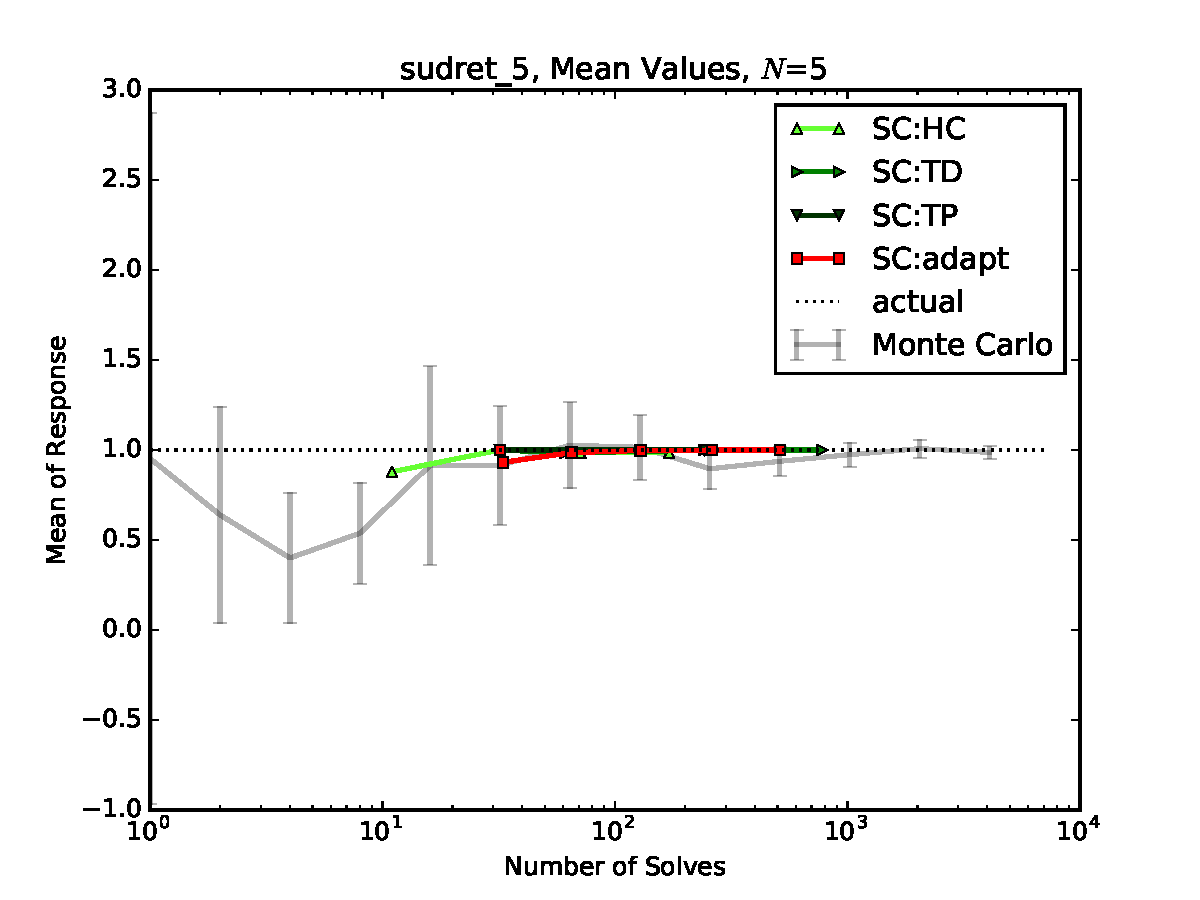
\includegraphics[width=0.7\linewidth]{anlmodels/sudret_5_mean_vals_nohdmr}
  \caption{Sudret Polynomial, $N=5$, Mean Values}
  \label{fig:sudretpoly mean values 5}
\end{figure}
\begin{figure}[H]
  \centering
  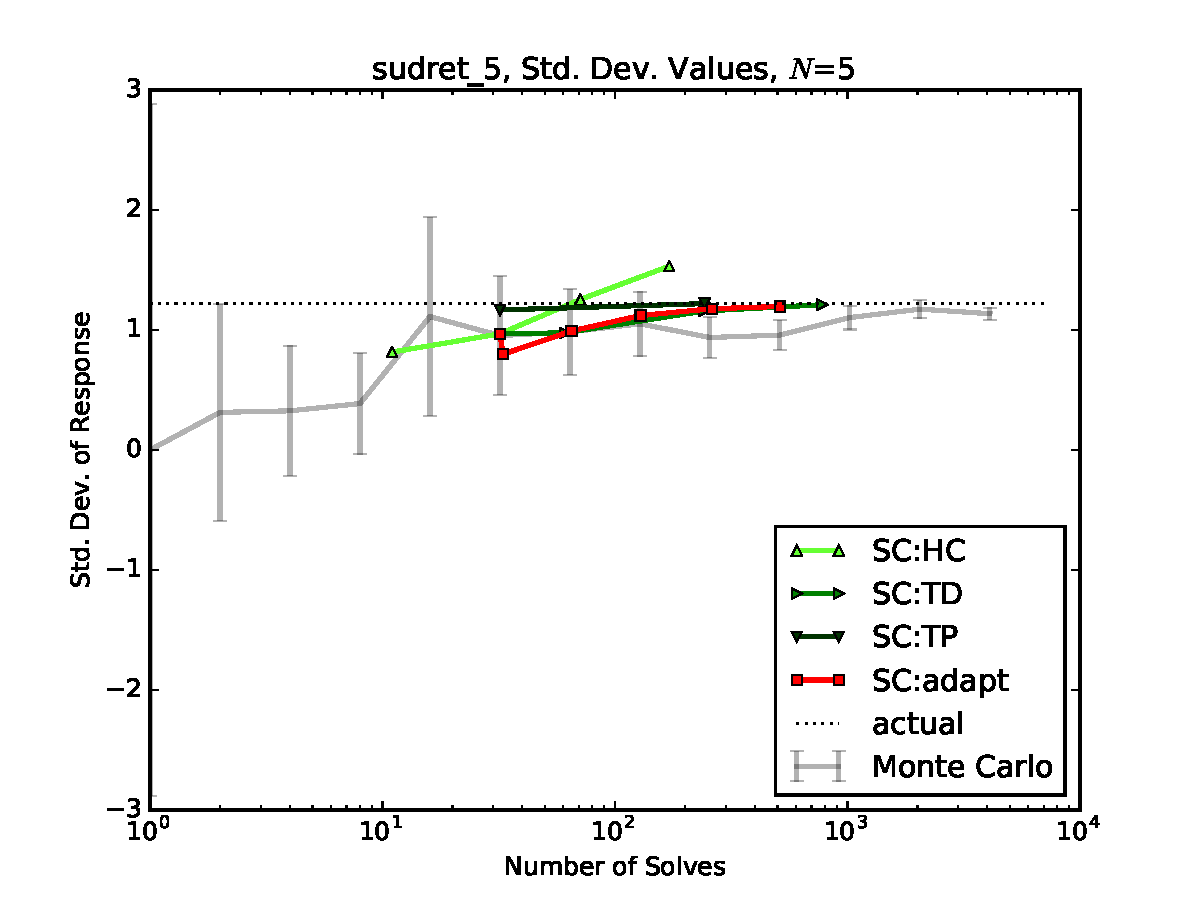
\includegraphics[width=0.7\linewidth]{anlmodels/sudret_5_var_vals_nohdmr}
  \caption{Sudret Polynomial, $N=5$, Std. Dev. Values}
  \label{fig:sudretpoly var values 5}
\end{figure}

\begin{figure}[H]
  \centering
  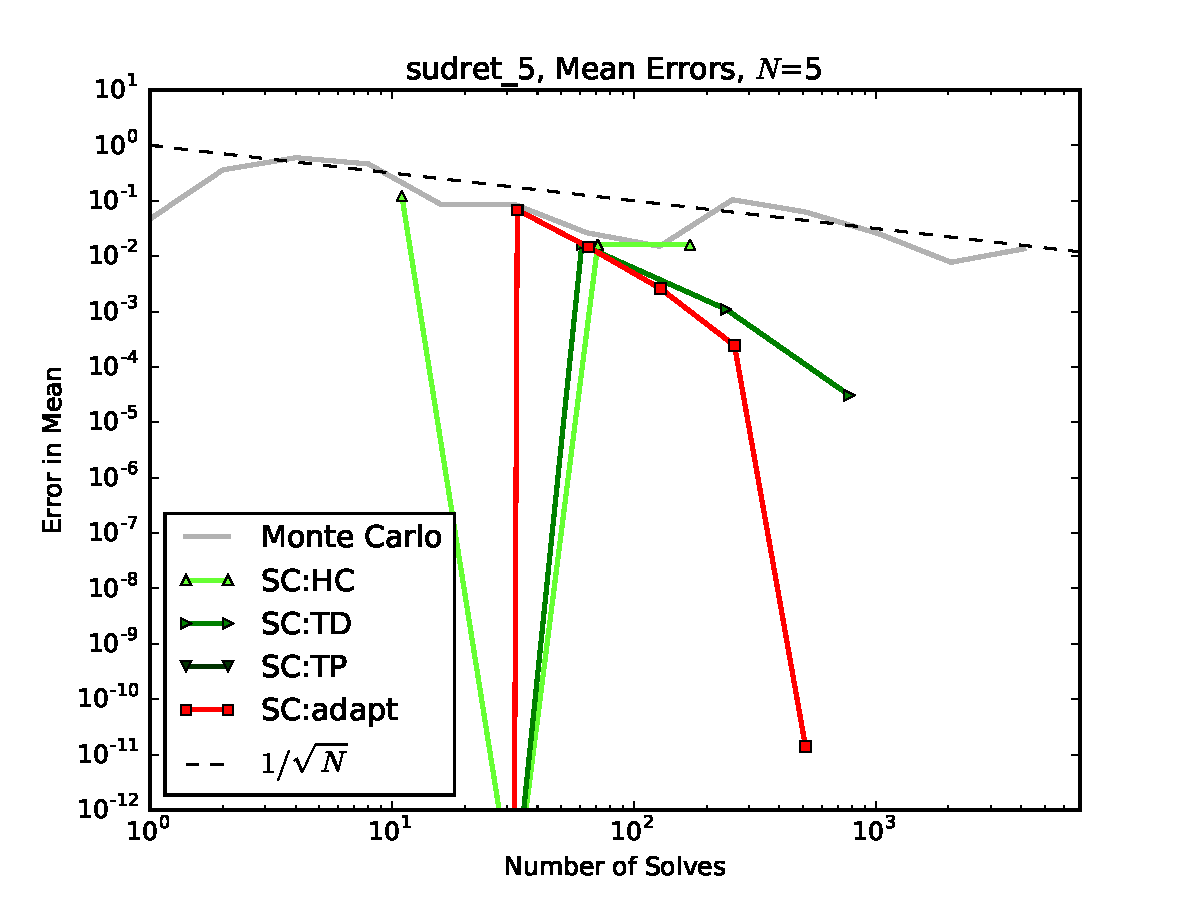
\includegraphics[width=0.7\linewidth]{anlmodels/sudret_5_mean_errs_nohdmr}
  \caption{Sudret Polynomial, $N=5$, Mean Convergence}
  \label{fig:sudretpoly mean errors 5}
\end{figure}
\begin{figure}[H]
  \centering
  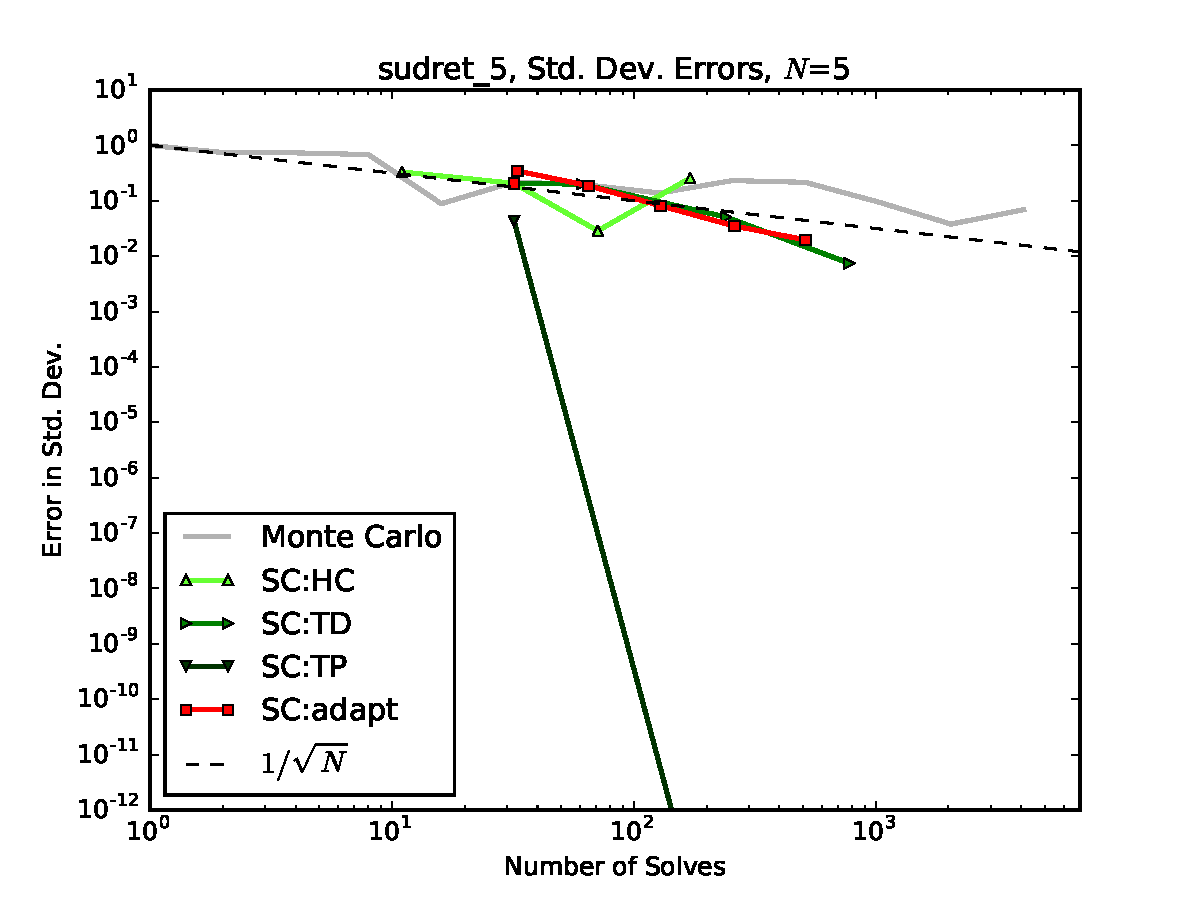
\includegraphics[width=0.7\linewidth]{anlmodels/sudret_5_variance_errs_nohdmr}
  \caption{Sudret Polynomial, $N=5$, Std. Dev. Convergence}
  \label{fig:sudretpoly var errors 5}
\end{figure}


\section{Attenuation}
\subsection{Description}\label{mod:attenuation}
While this model is effectively a tensor product of polynomials and has an analytic response, 
it also is the model for a common physical problem.
Consider a one-dimensional geometry that consists of a material with unit length and vacuum to the left and
right of the material.  We consider a beam of neutral particles that have a probability of interacting
with the material through absorption, or passing through it.  This beam enters the material on the left
and exits on the right with a fraction of its original flux.  See for example Figure \ref{fig: atten}, where
the dark arrows represent beam travel direction and their thickness generally depicts the beam attenuating
through the material.  The spatial domain is [0,1].
The quantity of interest is the percent of particles that pass through the material without interacting
anywhere along its length.  The boundary conditions for this problem are a constant positive current on the 
left boundary, and a vacuum on the right boundary.
\begin{figure}[htb]
  \centering
  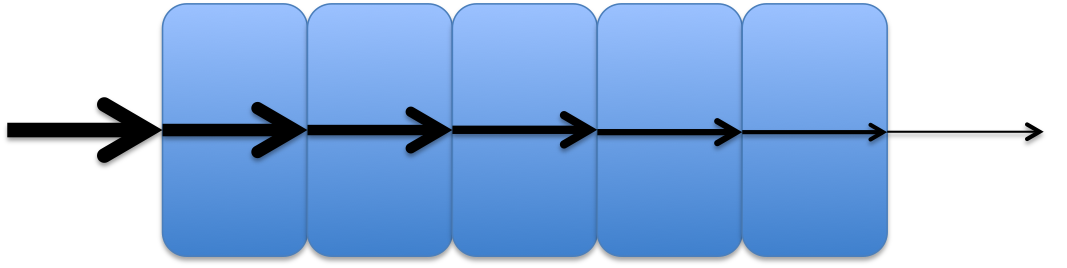
\includegraphics[width=0.7\linewidth]{attenuate}
  \caption{Attenuation Model Visualization ($N=5$)}
  \label{fig: atten}
\end{figure}

This model represents the idealized single-dimension system where an beam of particles impinges on a
purely-absorbing material with total scaled length of 1.
The material is divided into $N$ segments, each of which
has a distinct uncertain interaction cross section $y_n$.  The cross section has units of probable interactions
per unit length, and the integral of a cross section over a length provides the probability of interaction
within that length.  The response (percent of the beam to pass out the right boundary) takes the form
\begin{equation}
  u(Y) = \prod_{n=1}^N \exp(-y_n/N).
\end{equation}
The two-dimensional representation of this response is given in Figure \ref{fig: attenuation}.
\begin{figure}[htb]
  \centering
  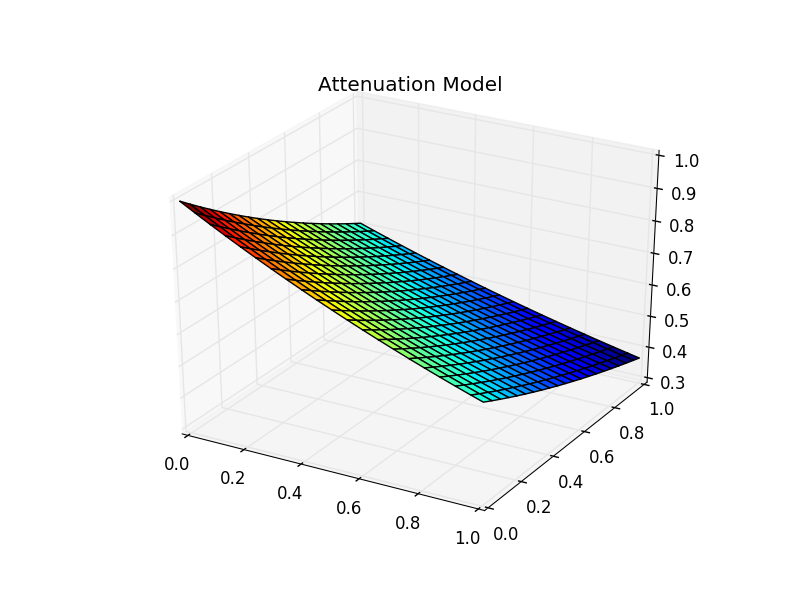
\includegraphics[width=0.7\linewidth]{anlmodels/attenuate}
  \caption{Attenuation Model Response}
  \label{fig: attenuation}
\end{figure}
Because negative cross sections have dubious physical meaning, we restrict the distribution cases to uniform
on [0,1] as well as normally-distributed on [$\mu,\sigma$].  A summary of analytic statistics is given in
Table \ref{tab:attenuation moments}.

\begin{table}[H]
  \centering
  \begin{tabular}{c|c|c}
    Distribution & Mean & Variance \\\hline
    $\mathcal{U}[0,1]$ & $\qty[N\qty(1-e^{-1/N})]^N$ & $\qty[\frac{N}{2}\qty(1-e^{-2/N})]^N -
                       \qty[N\qty(1-e^{-1/N})]^{2N}$ \\
    $\mathcal{N}[\mu,\sigma]$ & $\prod_{n=1}^N \exp\qty[\frac{\sigma_{y_n}^2}{2N^2}-\frac{\mu_{y_n}}{N}]$
    & $\prod_{n=1}^N \exp\qty[\frac{2\sigma_{y_n}^2}{N^2} - \frac{2\mu_{y_n}}{N}]$
  \end{tabular}
  \caption{Analytic Expressions for Attenuation Case}
  \label{tab:attenuation moments}
\end{table}

\subsection{Discussion}
This model has some interesting properties to demonstrate performance of polynomial-based UQ methods.  First,
because the solution is a product of exponential functions, it cannot be exactly represented by a finite
number of polynomials.  Second, the Taylor development of the exponential function (about the origin) 
includes all increasing polynomial orders,
\begin{equation}
e^{-ay} = 1 - ay + \frac{(ay)^2}{2} - \frac{(ay)^3}{6} + \frac{(ay)^4}{24} - \frac{(ay)^5}{120} + \mathcal{O}(y^6).
\end{equation}
As a result, the product of several exponential functions is effectively a tensor combination of
polynomials for each dimension.  The coefficients of higher-order polynomials are smaller than lower-order
polynomials.  Further, coefficients for combined polynomials 
have larger coefficients than single-dimensional
polynomials with the same effective order.  For example, for a two-dimensional exponential function and
considering effective fourth-order polynomials, the coefficient for $y_1^2y_2^2$ is $a^4/4$, while the
coefficient for $y_1^4$ is $a^4/24$.  This is shown graphically in Table \ref{tab:atten coeffs}.  The
magnitude of each coefficient for the tensor product of two Taylor expansions of the exponential function are
given tabularly.  The grayed entries are those for which the total polynomial order is four.  We can see
that the coefficients for polynomials equally split between the two input variables have a smaller denominator than
those made up entirely of one input variable, and so those that are equal in both dimensions are more
important to include in the expansion than those that are solely of one order or another.
\begin{table}
  \centering
  \begin{tabular}{|c c|c c c c c|}
    \cline{3-7}\multicolumn{2}{c|}{ } & \multicolumn{5}{c|}{Polynomial Order ($y_1$)} \\
               \multicolumn{2}{c|}{ } & 0 & 1 & 2 & 3 & 4 \\
    \hline & 0 & 1        & $a$      & $a^2/2$  & $a^3/6$   & \cellcolor{Gray6}$a^4/24$  \\
Polynomial & 1 & $a$      & $a^2   $ & $a^3/2 $ & \cellcolor{Gray6}$a^4/6  $ & $a^5/24 $ \\
Order      & 2 & $a^2/2$  & $a^3/2 $ & \cellcolor{Gray6}$a^4/4 $ & $a^5/12 $ & $a^6/48 $ \\
($y_2$)    & 3 & $a^3/ 6$ & \cellcolor{Gray6}$a^4/ 6$ & $a^5/12$ & $a^6/ 36$ & $a^7/144$ \\
           & 4 & \cellcolor{Gray6}$a^4/24$ & $a^5/24$ & $a^6/48$ & $a^7/144$ & $a^8/576$ \\
    \hline
  \end{tabular}
  \caption{Coefficient Magnitudes, Tensor Taylor Development of $e^{-ay}$}
  \label{tab:atten coeffs}
\end{table}
Note that in our case, $a=1/N$, which causes the polynomial coefficients to drop off more quickly, so that
low-order polynomial orders are more important to the expansion.  As a result, we see good convergence from the
collocation methods generally.

\subsection{Attenuation: 2 Inputs}
With only two input parameters, we see excellent convergence for all methods in the response mean, while Hyperbolic
Cross struggles to accurately represent the standard deviation.  As mentioned in the description, this is
likely because monomials are less important in the Taylor representation, while Hyperbolic Cross emphasizes
monomials over cross terms.  Interestingly, while Tensor
Product demonstrates the smallest error, its apparent curvature is slightly larger than for the other methods.
Because of the small input space, the total degree, hyperbolic cross, and adaptive methods all perform
similarly.  Because the adaptive method uses the impact of previous polynomials to choose future polynomials,
its convergence rate appears to improve as it continues.
\begin{figure}[H]
  \centering
  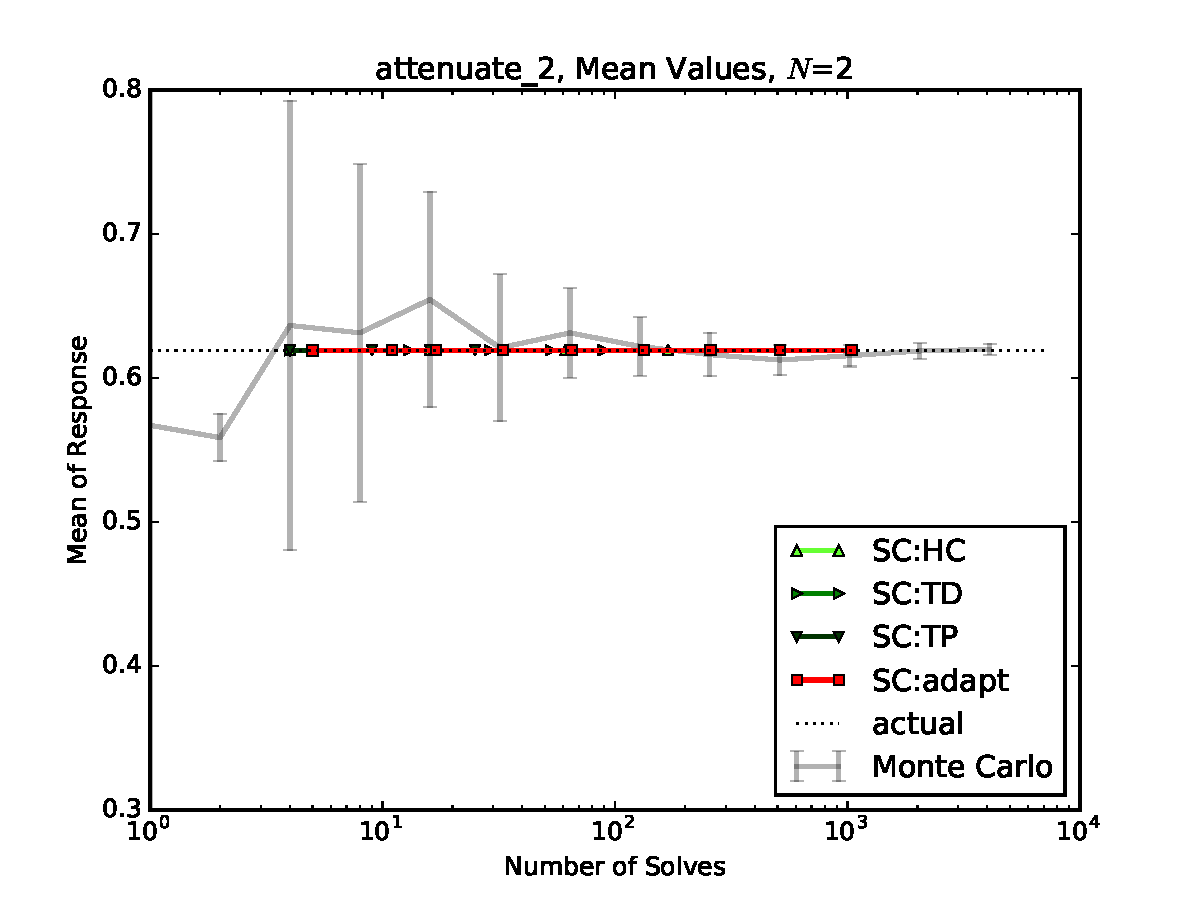
\includegraphics[width=0.7\linewidth]{anlmodels/attenuate_2_mean_vals_nohdmr}
  \caption{Attenuation, $N=2$, Mean Values}
  \label{fig:attenuate mean values 2}
\end{figure}
\begin{figure}[H]
  \centering
  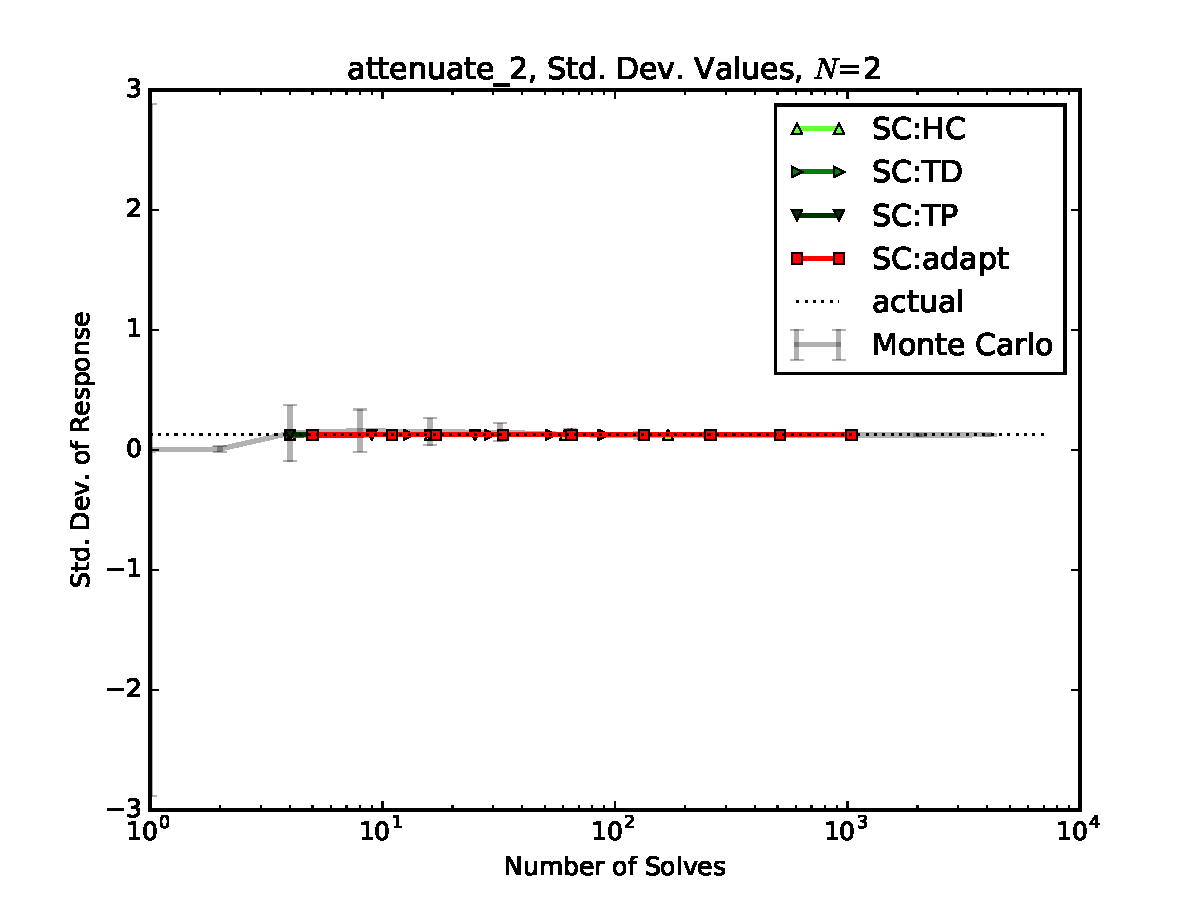
\includegraphics[width=0.7\linewidth]{anlmodels/attenuate_2_var_vals_nohdmr}
  \caption{Attenuation, $N=2$, Std. Dev. Values}
  \label{fig:attenuate var values 2}
\end{figure}

\begin{figure}[H]
  \centering
  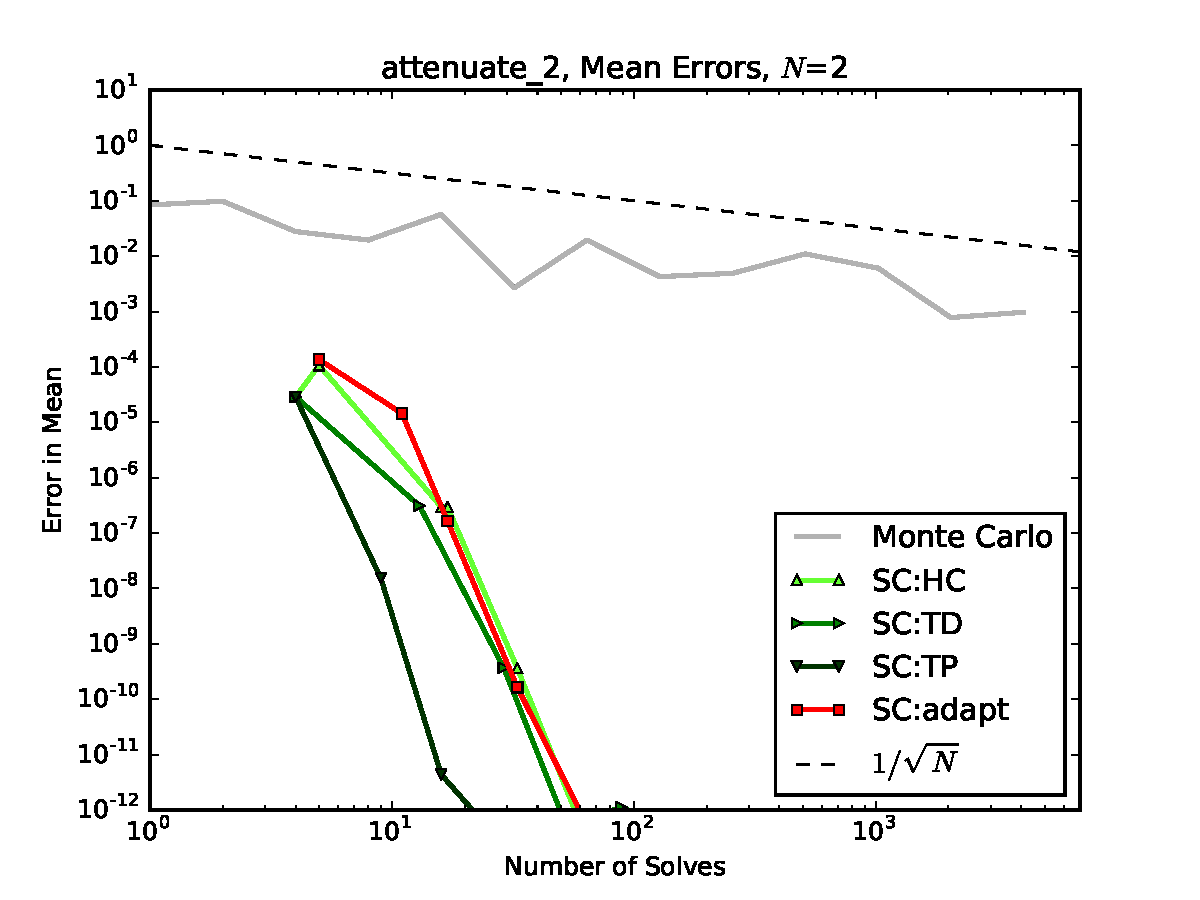
\includegraphics[width=0.7\linewidth]{anlmodels/attenuate_2_mean_errs_nohdmr}
  \caption{Attenuation, $N=2$, Mean Convergence}
  \label{fig:attenuate mean errors 2}
\end{figure}
\begin{figure}[H]
  \centering
  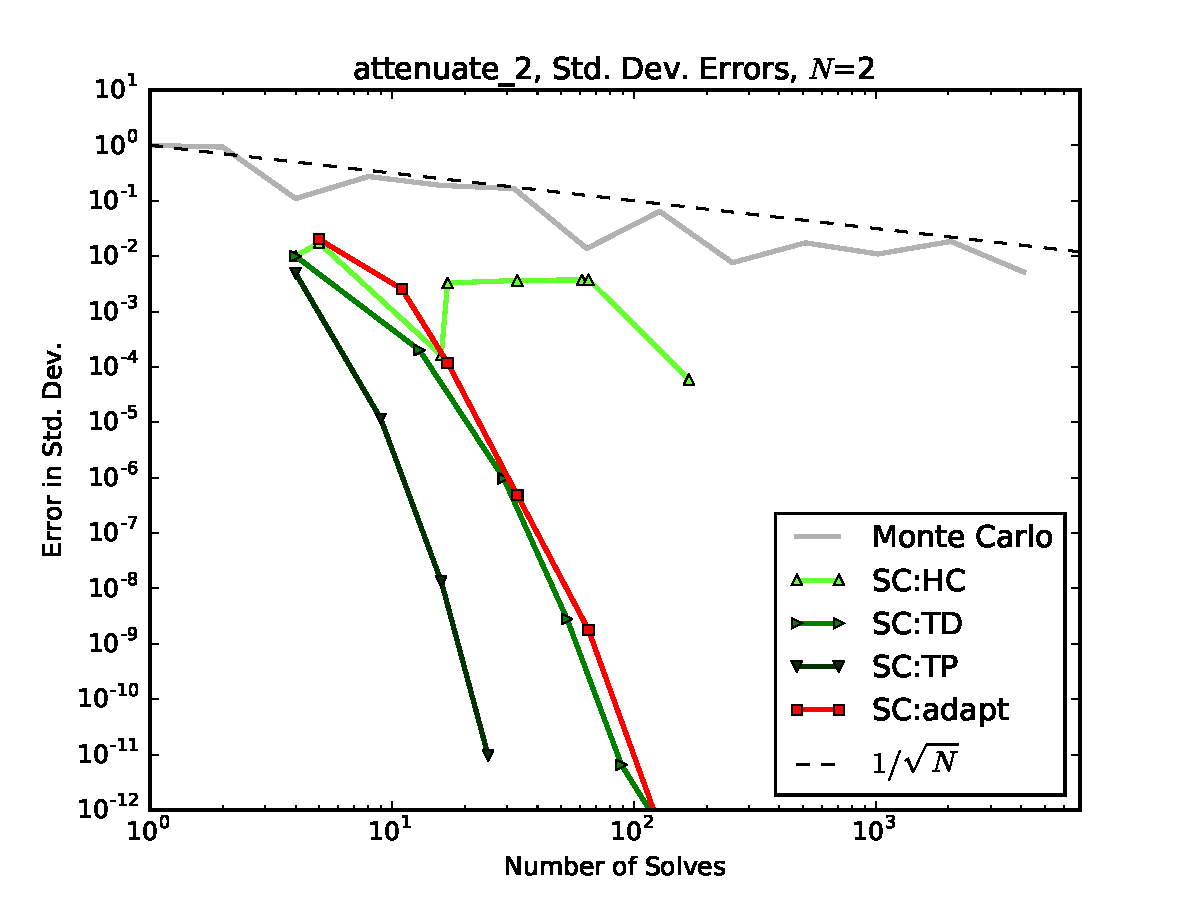
\includegraphics[width=0.7\linewidth]{anlmodels/attenuate_2_variance_errs_nohdmr}
  \caption{Attenuation, $N=2$, Std. Dev. Convergence}
  \label{fig:attenuate var errors 2}
\end{figure}


\subsection{Attenuation: 4 Inputs}
As with the two-input case, all methods show good convergence on the mean, and only the Hyperbolic Cross
polynomials show poor performance for the standard deviation.  Interestingly, despite Tensor Product matching
the construction shape of the model well, both Total Degree and Adaptive perform quite similar to TP and converge
quickly as well.
\begin{figure}[H]
  \centering
  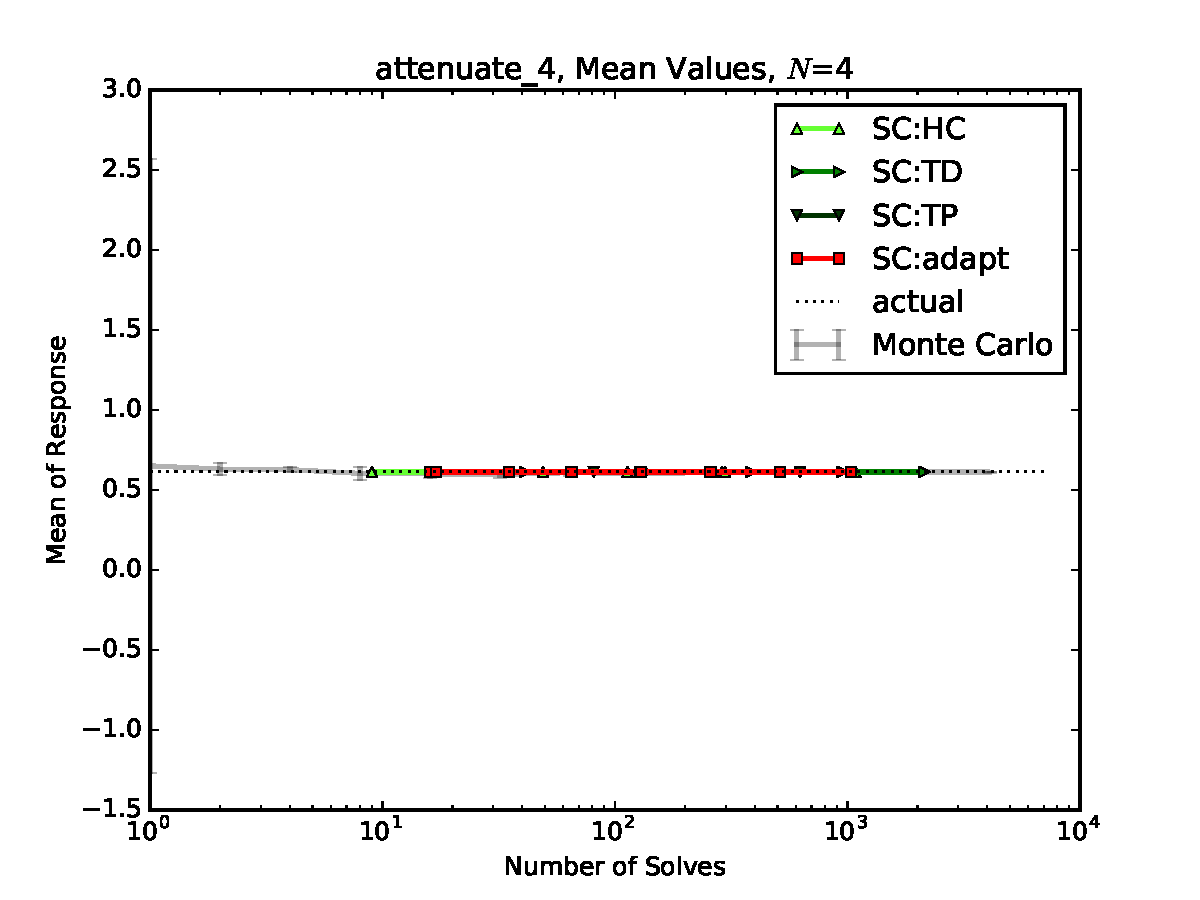
\includegraphics[width=0.7\linewidth]{anlmodels/attenuate_4_mean_vals_nohdmr}
  \caption{Attenuation, $N=4$, Mean Values}
  \label{fig:attenuate mean values 4}
\end{figure}
\begin{figure}[H]
  \centering
  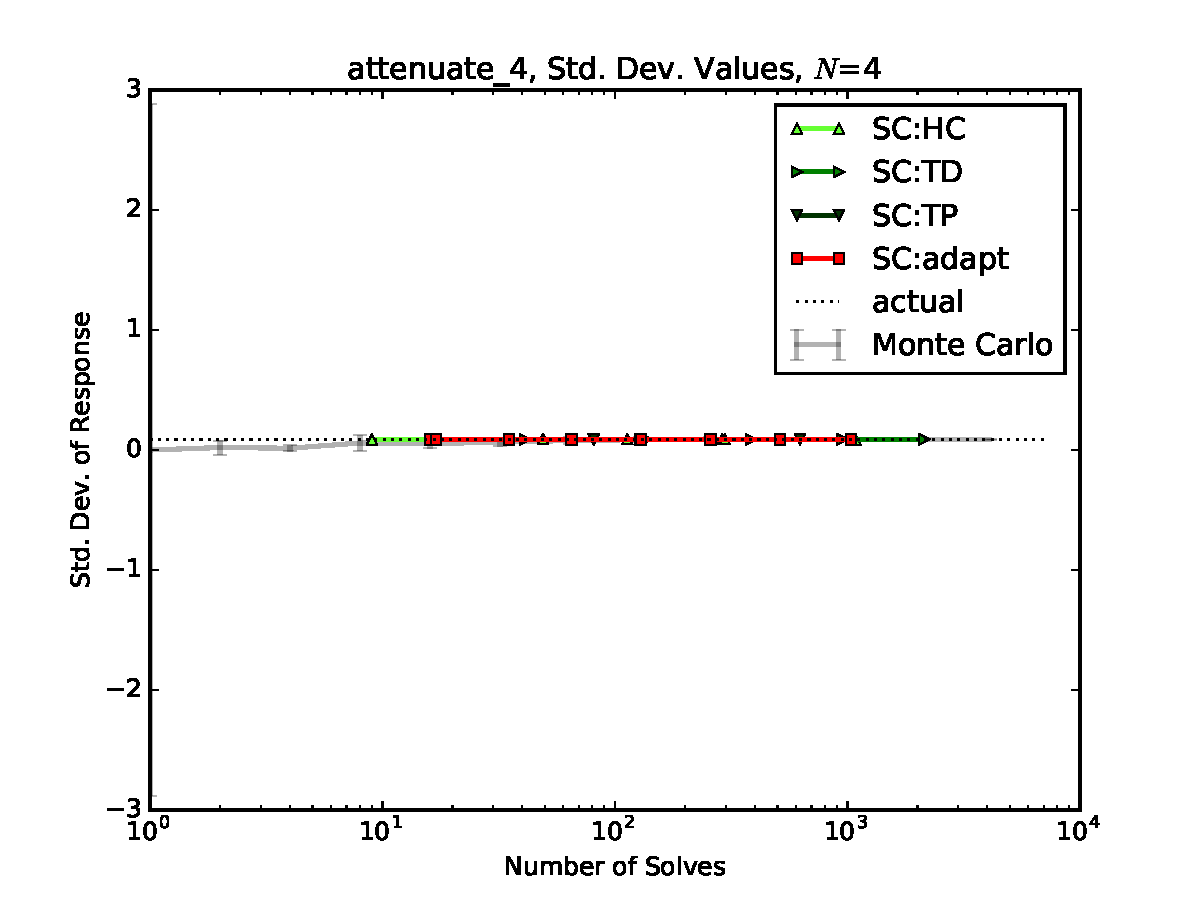
\includegraphics[width=0.7\linewidth]{anlmodels/attenuate_4_var_vals_nohdmr}
  \caption{Attenuation, $N=4$, Std. Dev. Values}
  \label{fig:attenuate var values 4}
\end{figure}

\begin{figure}[H]
  \centering
  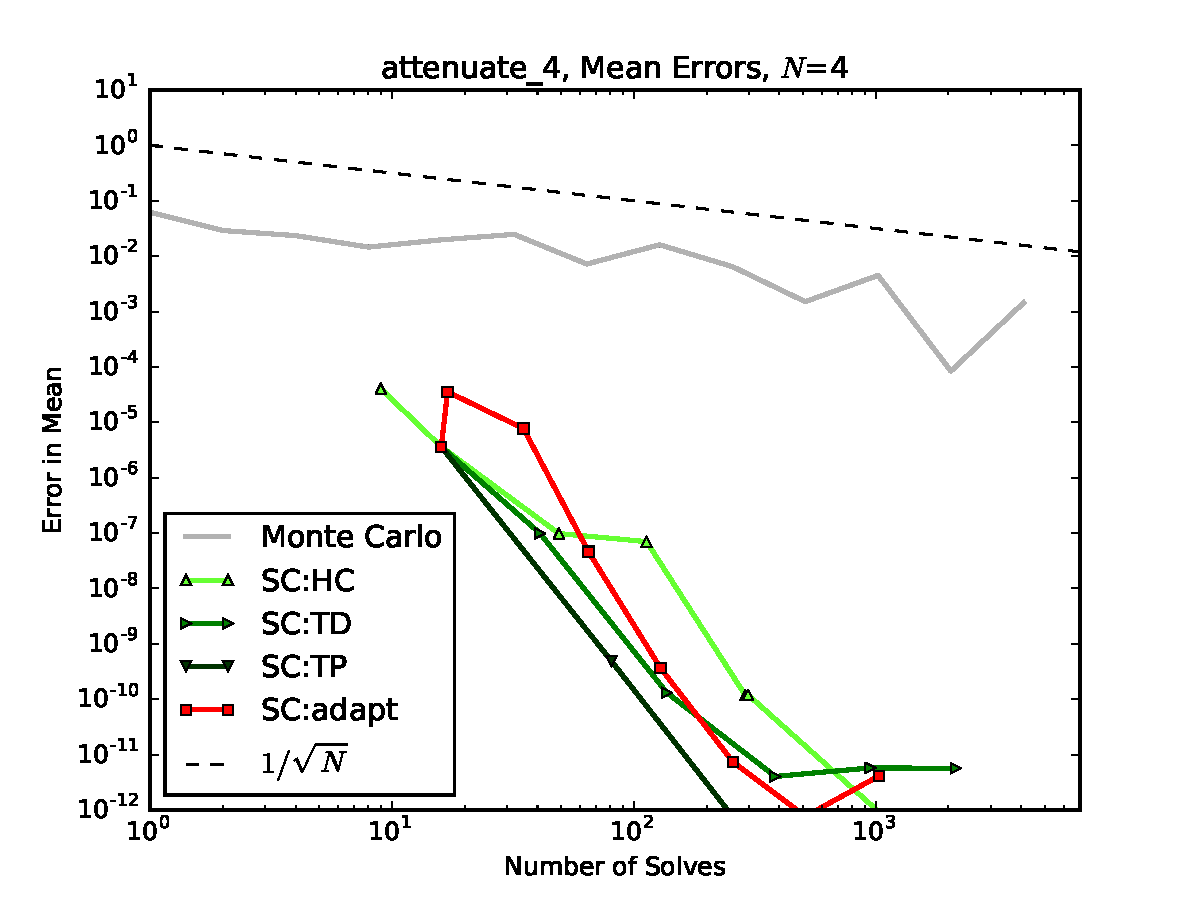
\includegraphics[width=0.7\linewidth]{anlmodels/attenuate_4_mean_errs_nohdmr}
  \caption{Attenuation, $N=4$, Mean Convergence}
  \label{fig:attenuate mean errors 4}
\end{figure}
\begin{figure}[H]
  \centering
  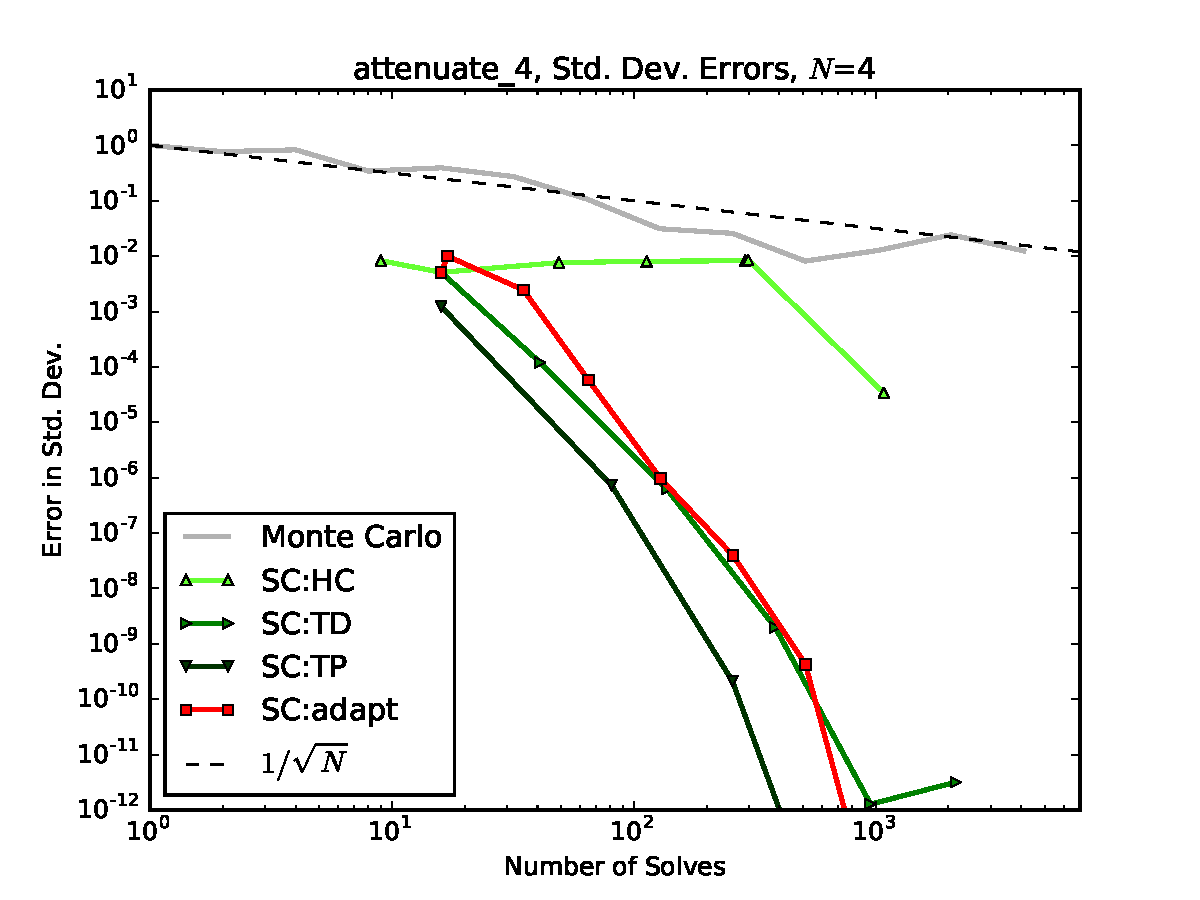
\includegraphics[width=0.7\linewidth]{anlmodels/attenuate_4_variance_errs_nohdmr}
  \caption{Attenuation, $N=4$, Std. Dev. Convergence}
  \label{fig:attenuate var errors 4}
\end{figure}

\subsection{Attenuation: 6 Inputs}
The general trend in the two-input and four-input cases continues for six inputs, with one exception.  For six
inputs, the Adaptive method struggles to find the most suitable set of polynomials to include in the
expansion.  This is likely because of the large number of polynomial combinations available to consider 
with the larger input space.  If there is any tendency to inaccurately guess the path to take, this misstep is
likely to be taken many times before the more accurate path is discovered.  Otherwise, exponential convergence
is still observed, but with a larger radius of curvature than the lower-dimension cases.
\begin{figure}[H]
  \centering
  \includegraphics[width=0.7\linewidth]{anlmodels/attenuate_6_mean_vals_nohdmr}
  \caption{Attenuation, $N=6$, Mean Values}
  \label{fig:attenuate mean values 6}
\end{figure}
\begin{figure}[H]
  \centering
  \includegraphics[width=0.7\linewidth]{anlmodels/attenuate_6_var_vals_nohdmr}
  \caption{Attenuation, $N=6$, Std. Dev. Values}
  \label{fig:attenuate var values 6}
\end{figure}

\begin{figure}[H]
  \centering
  \includegraphics[width=0.7\linewidth]{anlmodels/attenuate_6_mean_errs_nohdmr}
  \caption{Attenuation, $N=6$, Mean Convergence}
  \label{fig:attenuate mean errors 6}
\end{figure}
\begin{figure}[H]
  \centering
  \includegraphics[width=0.7\linewidth]{anlmodels/attenuate_6_variance_errs_nohdmr}
  \caption{Attenuation, $N=6$, Std. Dev. Convergence}
  \label{fig:attenuate var errors 6}
\end{figure}


\section{Gauss Peak}
\subsection{Description}\label{mod:gausspeak}
Similar to the attenuation model, the Gaussian peak \cite{sfugenz} instead uses square arguments to the
exponential function.  A tuning parameter $a$ can also be used to change the peakedness of the
function.  Increased peakedness leads to more difficult polynomial representation.
A location parameter $\mu$ can be used to change the location of the peak.
The mathematical expression is
\begin{equation}
  u(Y) = \exp\qty(-\sum_{n=1}^N a^2\qty(y_n-\mu)^2).
\end{equation}
We allow each $y_n$ to vary uniformly on [0,1] and set peakedness to $a=3$, with the center
of the peak at (0.5,0.5).
The two-dimensional representation of this response is given in Figure \ref{fig: gauss peak}.
\begin{figure}[htb]
  \centering
  \includegraphics[width=0.7\linewidth]{anlmodels/gaussian}
  \caption{Gaussian Peak Response \cite{sfu}}
  \label{fig: gauss peak}
\end{figure}
A summary of analytic statistics is given in Table \ref{tab:gausspeak moments}.

\begin{table}[H]
  \centering
  \begin{tabular}{c|c}
    Statistic & Expression \\ \hline
    Mean & $\qty(\frac{\sqrt{\pi}}{2a}\qty(\erf(a\mu)+\erf(a-a\mu)))^N$ \\
    Variance & $\qty(\frac{\sqrt{\pi/2}}{2a}\qty(\erf(a\mu\sqrt{2})-\erf(a\sqrt{2}(1-\mu))))^N - 
        \qty(\frac{\sqrt{\pi}}{2a}\qty(\erf(a\mu)+\erf(a-a\mu)))^{2N}$
  \end{tabular}
  \caption{Analytic Expressions for Gaussian Peak Case}
  \label{tab:gausspeak moments}
\end{table}
\subsection{Discussion}
This case offers particular challenge because of its Taylor development, which only includes even powers of
the uncertain parameters,
\begin{equation}\label{eq: taylor peak}
  e^{-a^2y^2} = 1 - a^2y^2 + \frac{a^4}{2}y^4 - \frac{a^6}{6}y^6 + \frac{a^8}{24}y^8 + \mathcal{O}(y^{10}).
\end{equation}
This suggests added difficulty in successive representation, especially for an
adaptive algorithm.  A visual demonstration of this is shown in Table
\ref{tab: gauss coeffs}.
\begin{table}
  \centering
  \begin{tabular}{|c c|c c c c c|}
    \cline{3-7}\multicolumn{2}{c|}{ } & \multicolumn{5}{c|}{Polynomial Order ($y_1$)} \\
\multicolumn{2}{c|}{ } & 0       & 1 & 2       & 3 & 4       \\
    \hline         & 0 & 1       & 0 & $a^2$   & 0 & $a^4/2$ \\ 
Polynomial         & 1 & 0       & 0 & 0       & 0 & 0       \\
Order              & 2 & $a^2$   & 0 & $a^4$   & 0 & $a^6/2$ \\
($y_2$)            & 3 & 0       & 0 & 0       & 0 & 0       \\
                   & 4 & $a^4/2$ & 0 & $a^6/2$ & 0 & $a^8/4$ \\
    \hline
  \end{tabular}
  \caption{Coefficient Magnitudes, Tensor Taylor Development of $e^{-a^2y^2}$}
  \label{tab: gauss coeffs}
\end{table}
This Taylor development shows the same tendencies as the Attenuation model Taylor development; however, only
even polynomials are present, and these drop off at a slower rate than the Attenuation model.  Also, because
$a$ is greater than one for this model, it counteracts the polynomial coefficient dropoff seen in the
expansion, whereas in the Attenuation model $a$ was less than one and coefficients dropped off more quickly as
a result.  Due to these factors, we see poorer performance for the collocation methods on converging this
model than the Attenuation model, despite their apparent similarities.

\subsection{Gauss Peak: 3 Inputs}
For this smaller input space, we see good exponential convergence on the mean for the Hyperbolic Cross, Total
Degree, and Tensor Product index sets.  However, the adaptive method fails entirely.  This is because none of
the first-order polynomials have any contribution even when integrated coarsely; as a result, the adaptive
algorithm is duped into believing it is converged.  This same behavior is seen for the five-input case as
well.  As expected, the standard deviation shows poorer performance for all three methods than the mean; in
fact, only the Tensor Product is clearly converging exponentially for the standard deviation even with only three inputs.
This demonstrates the challenge of this model to be represented well with low-order polynomials.
\begin{figure}[H]
  \centering
  \includegraphics[width=0.7\linewidth]{anlmodels/sfu_gauss_peak_3_mean_vals_nohdmr}
  \caption{Gauss Peak, $N=3$, Mean Values}
  \label{fig:gauss peak mean values 3}
\end{figure}
\begin{figure}[H]
  \centering
  \includegraphics[width=0.7\linewidth]{anlmodels/sfu_gauss_peak_3_var_vals_nohdmr}
  \caption{Gauss Peak, $N=3$, Std. Dev. Values}
  \label{fig:gauss peak var values 3}
\end{figure}

\begin{figure}[H]
  \centering
  \includegraphics[width=0.7\linewidth]{anlmodels/sfu_gauss_peak_3_mean_errs_nohdmr}
  \caption{Gauss Peak, $N=3$, Mean Convergence}
  \label{fig:gauss peak mean errors 3}
\end{figure}
\begin{figure}[H]
  \centering
  \includegraphics[width=0.7\linewidth]{anlmodels/sfu_gauss_peak_3_variance_errs_nohdmr}
  \caption{Gauss Peak, $N=3$, Std. Dev. Convergence}
  \label{fig:gauss peak var errors 3}
\end{figure}

\subsection{Gauss Peak: 5 Inputs}
The same trends are observed for five inputs as for three, but with poorer convergence in all methods.  While
it appears there is some exponential convergence benefits in the collocation methods, for up to 1000 computation solves
there is little advantage over MC.
\begin{figure}[H]
  \centering
  \includegraphics[width=0.7\linewidth]{anlmodels/sfu_gauss_peak_5_mean_vals_nohdmr}
  \caption{Gauss Peak, $N=5$, Mean Values}
  \label{fig:gauss peak mean values 5}
\end{figure}
\begin{figure}[H]
  \centering
  \includegraphics[width=0.7\linewidth]{anlmodels/sfu_gauss_peak_5_var_vals_nohdmr}
  \caption{Gauss Peak, $N=5$, Std. Dev. Values}
  \label{fig:gauss peak var values 5}
\end{figure}

\begin{figure}[H]
  \centering
  \includegraphics[width=0.7\linewidth]{anlmodels/sfu_gauss_peak_5_mean_errs_nohdmr}
  \caption{Gauss Peak, $N=5$, Mean Convergence}
  \label{fig:gauss peak mean errors 5}
\end{figure}
\begin{figure}[H]
  \centering
  \includegraphics[width=0.7\linewidth]{anlmodels/sfu_gauss_peak_5_variance_errs_nohdmr}
  \caption{Gauss Peak, $N=5$, Std. Dev. Convergence}
  \label{fig:gauss peak var errors 5}
\end{figure}




\section{Ishigami}
\subsection{Description}\label{mod:ishigami}
The Ishigami function \cite{ishigami} is a commonly-used function in performing sensitivity analysis.  It is
given by
\begin{equation}
  u(Y) = \sin{y_1} + a\sin^2{y_2} + b y_3^4\sin(y_1).
\end{equation}
In our case, we will use $a=7$ and $b=0.1$ as in \cite{ishigami2}.
The graphical representation of this response is given in Figure \ref{fig: ishigami}, with the three axes
as the three inputs and the color map as the function values ranging approximately from -10.74 to 17.74.
\begin{figure}[htb]
  \centering
  \includegraphics[width=0.7\linewidth]{anlmodels/ishigami}
  \caption{Ishigami Model Response}
  \label{fig: ishigami}
\end{figure}
In particular interest for this model are
its strong nonlinearity and lack of independence for $y_3$, as it only appears in conjunction with $y_1$.  The
analytic statistics of interest for this model are in Table \ref{tab:ishigami moments}, where $D_n$ is the
partial variance contributed by $y_n$ and Sobol sensitivities $\mathcal{S}_n$ are obtained by dividing $D_n$
by the total variance.

\begin{table}[H]
  \centering
  \begin{tabular}{c|c|c}
  Statistic & Expression & Approx. Value \\\hline
  Mean & $\frac{7}{2}$ & 3.5 \\
  Variance & $\frac{a^2}{8} + \frac{b\pi^4}{5} + \frac{b^2\pi^8}{18} + \frac{1}{2}$ & 13.84459 \\
  $D_1$ & $\frac{b\pi^4}{5} + \frac{b^2\pi^8}{50} + \frac{1}{2} $ &  4.34589 \\
  $D_2$ & $\frac{a^2}{8}$ & 6.125 \\
  $D_{1,3}$ & $\frac{8b^2\pi^8}{225}$ & 3.3737 \\
  $D_3,D_{1,2},D_{2,3},D_{1,2,3}$ & 0 & 0
  \end{tabular}
  \caption{Analytic Expressions for Ishigami Case}
  \label{tab:ishigami moments}
\end{table}


\subsection{Discussion}
The Ishigami function is sinusoidal in $y_1$ and $y_2$.  Because the sine function is exclusively odd, this presents
a similar challenge as previous models to adaptive methods, at least for these two dimensions.  $y_3$, however, only
appears as a fourth-order coefficient to the sine of $y_1$, which makes for a relationship that is difficult for the
polynomial representations to capture.  For this model, there is no flexibility in the dimensionality of the
input space; we show the only case ($N=3$) here.

\subsection{Ishigami: 3 Inputs}
For the mean we see good convergence for the three static methods, and surprisingly good convergence for the
Hyperbolic Cross polynomials.  Because the two dominant parameters are largely independent, the polar focus of
the Hyperbolic Cross set captures the essential components with less computation than the other two static
methods.  The adaptive method, as predicted, struggles to find any important polynomials before finding false
convergence.

For the standard deviation, however, we see significant divergence for both the Hyperbolic Cross and Adaptive
methods.  Despite some oscillations, however, we do see exponential convergence for both the Tensor Product
and Total Degree methods.  Despite this, marked improvements over MC are not distinct until after 100
computational solves, despite the small input space.
\begin{figure}[H]
  \centering
  \includegraphics[width=0.7\linewidth]{anlmodels/ishigami_3_mean_vals_nohdmr}
  \caption{Ishigami, $N=3$, Mean Values}
  \label{fig:ishigami mean values 3}
\end{figure}
\begin{figure}[H]
  \centering
  \includegraphics[width=0.7\linewidth]{anlmodels/ishigami_3_var_vals_nohdmr}
  \caption{Ishigami, $N=3$, Std. Dev. Values}
  \label{fig:ishigami var values 3}
\end{figure}

\begin{figure}[H]
  \centering
  \includegraphics[width=0.7\linewidth]{anlmodels/ishigami_3_mean_errs_nohdmr}
  \caption{Ishigami, $N=3$, Mean Convergence}
  \label{fig:ishigami mean errors 3}
\end{figure}
\begin{figure}[H]
  \centering
  \includegraphics[width=0.7\linewidth]{anlmodels/ishigami_3_variance_errs_nohdmr}
  \caption{Ishigami, $N=3$, Std. Dev. Convergence}
  \label{fig:ishigami var errors 3}
\end{figure}


\section{Sobol G-Function}
\subsection{Description}\label{mod:gfunc}
The so-called ``g-function'' introduced by Saltelli and Sobol \cite{gfunc} is a discontinuous
function used most commonly as a test for sensitivity coefficients.  The function is often used as an integrand
for numerical estimation methods \cite{gfuncM}.
The function is given by
\begin{equation}
  u(Y) = \prod_{n=1}^N \frac{\abs{4y_n-2}-a_n}{1+a_n},
\end{equation}
where
\begin{equation}
  a_n = \frac{n-2}{2}.
\end{equation}
The two-dimensional representation of this response is given in Figure \ref{fig: g func}.
\begin{figure}[htb]
  \centering
  \includegraphics[width=0.7\linewidth]{anlmodels/gfunc}
  \caption{Sobol G-Function Response \cite{sfu}}
  \label{fig: g func}
\end{figure}

There are some implementations \cite{gfuncM} that force $a_n \geq 0$, which allows for a simple
understanding of the sensitivity coefficients:
\begin{itemize}
  \item $a_n=0$: $y_n$ is very important
  \item $a_n=1$: $y_n$ is relatively important,
  \item $a_n=9$: $y_n$ is non-important,
  \item $a_n=99$: $y_n$ is non-significant.
\end{itemize}
However, for our purposes, we set no limit to the value of $a_n$, as our interest is primarily in the moments
instead of the sensitivity coefficients.

We select this model because it offers the challenge of a function
without a continuous first derivative.  We expect the polynomial representations to perform poorly
in this instance, and more so as dimensionality increases.

\subsection{Discussion}
As expected, even for 3 input variables this discontinuous model provides a difficult challenge for
polynomial representations.  Despite thousands of computational solves, there is no discernible benefit in using
collocation methods over traditional MC.  As with the Gaussian peak, the adaptive method completely
stalls in trying to converge this model.
\subsection{Sobol G-Function: 3 Inputs}
As evidenced in the figures, there is little justification for using any of the collocation methods for
uncertainty quantification with this model.  The level of discontinuity renders the benefits of the polynomial
expansions moot.
\begin{figure}[H]
  \centering
  \includegraphics[width=0.7\linewidth]{anlmodels/sobolG_3_mean_vals_nohdmr}
  \caption{Sobol G-Function, $N=3$, Mean Values}
  \label{fig:sobolG mean values 3}
\end{figure}
\begin{figure}[H]
  \centering
  \includegraphics[width=0.7\linewidth]{anlmodels/sobolG_3_var_vals_nohdmr}
  \caption{Sobol G-Function, $N=3$, Std. Dev. Values}
  \label{fig:sobolG var values 3}
\end{figure}

\begin{figure}[H]
  \centering
  \includegraphics[width=0.7\linewidth]{anlmodels/sobolG_3_mean_errs_nohdmr}
  \caption{Sobol G-Function, $N=3$, Mean Convergence}
  \label{fig:sobolG mean errors 3}
\end{figure}
\begin{figure}[H]
  \centering
  \includegraphics[width=0.7\linewidth]{anlmodels/sobolG_3_variance_errs_nohdmr}
  \caption{Sobol G-Function, $N=3$, Std. Dev. Convergence}
  \label{fig:sobolG var errors 3}
\end{figure}

\subsection{Sobol G-Function: 5 Inputs}
As with the smaller input space, it is clear that discontinuous models such as this are poor candidates for
collocation-based uncertainty analysis.
\begin{figure}[H]
  \centering
  \includegraphics[width=0.7\linewidth]{anlmodels/sobolG_5_mean_vals_nohdmr}
  \caption{Sobol G-Function, $N=5$, Mean Values}
  \label{fig:sobolG mean values 5}
\end{figure}
\begin{figure}[H]
  \centering
  \includegraphics[width=0.7\linewidth]{anlmodels/sobolG_5_var_vals_nohdmr}
  \caption{Sobol G-Function, $N=5$, Std. Dev. Values}
  \label{fig:sobolG var values 5}
\end{figure}

\begin{figure}[H]
  \centering
  \includegraphics[width=0.7\linewidth]{anlmodels/sobolG_5_mean_errs_nohdmr}
  \caption{Sobol G-Function, $N=5$, Mean Convergence}
  \label{fig:sobolG mean errors 5}
\end{figure}
\begin{figure}[H]
  \centering
  \includegraphics[width=0.7\linewidth]{anlmodels/sobolG_5_variance_errs_nohdmr}
  \caption{Sobol G-Function, $N=5$, Std. Dev. Convergence}
  \label{fig:sobolG var errors 5}
\end{figure}




\section{Conclusions}
We have demonstrated the performance of SCgPC using a variety of polynomial set construction techniques
described in Chapter \ref{ch:methods scgpc}: tensor product, total degree, and hyperbolic cross, as well as
adaptive.  There are several conclusions that can be drawn from these models.

First, in all cases the ability of collocation-based methods to be efficient in converging second-order
statistics was reduced in direct correlation with the dimensionality of the input space.  For an input space
of five or less variables, in general the collocation methods performed well, while for more than five
variables, performance was degraded significantly.

Second, as a model demonstrates less regularity, the performance of SCgPC methods in comparison to MC
degrades.  In the case of the Sobol G-Function, which is only zeroth-order continuous, SCgPC fails to offer
any benefits over MC.  However, in models with more smoothness, in general SCgPC converged exponentially on
the response statistics.

The combination of dimensionality and smoothness can be seen through the several models presented.
The Tensor Monomials and Attenuation models demonstrate performance of collocation methods on
tensor-construction models with polynomial representations whose coefficient magnitudes are monotonically 
decreasing; that is, there
are no polynomial order coefficients which are zero, and each polynomial coefficient of a higher order is
smaller than one of a lower order.  In these conditions, all the collocation methods performed very well for
reasonably-sized input spaces.

The Sudret Polynomial and Gauss Peak models represent functions in which there are ``missing'' polynomial
orders; that is, there are some polynomial orders whose coefficients are zero, while higher-order polynomials
have nonzero coefficients.  These presented a greater challenge to the SCgPC methods, especially the adaptive
method.  Because the adaptive method uses lower-order coefficients to predict higher-order impacts, these
missing polynomials cause poor performance in the search algorithm.  In particular for the Gauss Peak model,
the high-order polynomials drop off slowly in importance, making polynomial representation costly.

The Ishigami function demonstrates performance when there is an irregular relationship between the input
variables and the response.  While two of the static methods (total degree and tensor product) demonstrated
good exponential convergence, the adaptive method was not convergent.  Finally, in the Sobol G-Function,
we saw that even first-order tensor polynomials, when made zeroth-order
continuous, are very difficult for SCgPC methods to converge.

In conclusion, the SCgPC methods excel when the input space is of small dimensionality and the response is
regular with respect to the input space.  The adaptive method performs well when the polynomial representation
of the response has monotonically decreasing reliance on increasing polynomial orders.  SCgPC methods also
perform especially well when the model is represented well by relatively low-order polynomials.  SCgPC methods
should not be used on discontinuous responses or models with large input space dimensionality, as MC is a more
practical tool to converge second-order statistics for such models.
 % 3 
% Chapter Template

\chapter{Methods: High-Density Model Reduction} % Main chapter title

\label{ch:methods hdmr} % Change X to a consecutive number; for referencing this chapter elsewhere, use \ref{ChapterX}

\lhead{Chapter 5. \emph{Methods: High Density Model Reduction}} % Change X to a consecutive number; this is for the header on each page - perhaps a shortened title

%----------------------------------------------------------------------------------------
%	SECTION: INTRO
%----------------------------------------------------------------------------------------

\section{Introduction}
TODO



\section{High-Dimension Model Representation (HDMR)}
While using SCgPC is one method for creating a reduced-order model for a simulation code $u(Y)$, another
useful model reduction is HDMR\cite{hdmr}, sometimes known as Sobol decomposition because the expansion is
conducive to easily determining Sobol sensitivity coefficients.  HDMR is an ANalysis Of VAriance (ANOVA)
method.

In general, the HDMR expansion involves the sum of several terms, each of which only depends on a subset of
the full input space.  The subsets are developed by integrating out the undesired dimensions.  Letting $H(Y)$
represent the untruncated HDMR expansion of $u(Y)$,
\begin{equation}\label{eq:anova}
  u(Y) = H(Y) = h_0 + \sum_{n=1}^N h_n + \sum_{n_1=1}^N \sum_{n_2=1}^{n_1-1} h_{n_1,n_2} + \cdots +
  h_{1,2,\ldots,N},
\end{equation}
where the expectation value $h_0$ is given by
\begin{align}\label{eq:hdmr 0}
  h_0 &\equiv \int_{\Omega_1} \rho_1(y_1)\ldots\int_{\Omega_N} \rho_N(y_N) u(y_1,\ldots,y_N)\ dy_1\ldots\ dy_N, \\
    &= \int_\Omega \rho(Y) u(Y) dY,
\end{align}
where $\Omega$ denotes the uncertainty space spanned by $Y$ and $\rho(Y)$ is the multidimensional probability distribution
function of $Y$. The first-order expansion terms $h_n$ are integrated as
\begin{equation}\label{eq:hdmr 1}
  h_n(y_n) \equiv \int_{\hat\Omega_n} \hat\rho_n(\hat Y_n) u(Y)\ d\hat Y_n - h_0,
\end{equation}
where we use ``hat'' notation to refer to all elements except the one listed; for example,
\begin{equation}
  \hat Y_n \equiv (y_1,\cdots,y_{n-1},y_{n+1},\cdots,y_N),
\end{equation}
\begin{equation}
  \hat Y_{m,n} \equiv (y_1,\cdots,y_{m-1},y_{m+1},\cdots,y_{n-1},y_{n+1},\cdots,y_N).
\end{equation}
Second and higher-order HDMR expansion terms are defined as
\begin{equation}\label{eq:hdmr 2}
  h_{n_1,n_2}(y_{n_1},y_{n_2})) \equiv \int_{\hat\Omega_{n_1,n_2}} \hat\rho_{n_1,n_2}(\hat Y_{n_1,n_2}) u(Y)\
      d\hat Y_{n_1,n_2} - h_{n_1} - h_{n_2} - h_0,
\end{equation}
and so on.

There are many useful properties of this generic HDMR expansion.  First, each term represents the contribution
of that subset to the original response; that is, $h_1$ provides the contributions to the response solely
from variable $y_1$.  Further, the total contribution of a variable is the sum of all subsets for whom
variable is part of the subspace.  For example, the total contribution of $y_1$ to the response is the sum of
contributions from $h_1,(h_1,h_2),\cdots,(h_1,h_2,h_3)$, etc.

Second, the individual terms in the HDMR expansion are orthogonal with respect to the probability weight over
the input space; that is,
\begin{equation}
  \int_\Omega h_a h_b dY = 0 \hspace{10pt}\forall\hspace{5pt} a\neq b.
\end{equation}
Because of this, the second statistical moment of the HDMR expansion with respect to any subset dimension is
the equivalent to the second statistical moment of the associated subset,
\begin{equation}
  \int_{\Omega_n} H(Y)^2 dy_n = \int_{\Omega_n} h_n^2 dy_n.
\end{equation}
This in turn yields Sobol sensitivity coefficients.  Sobol sensitivity coefficients measure the impact on the
variance of a response as the result of changes in the variance of an input (or combination of inputs).  For
the HDMR expansion,
\begin{equation}
  \mathcal{S}_n \equiv \frac{\text{var}\qty[h_n]}{\text{var}\qty[H(Y)]},
\end{equation}
\begin{equation}
  \mathcal{S}_{m,n} \equiv \frac{\text{var}\qty[h_{m,n}]}{\text{var}\qty[H(Y)]},
\end{equation}
and so on.

\subsection{Cut-HDMR}\label{sec:cuthdmr}
The primary challenge in implementing HDMR for arbitrary responses is the integrals in Eq. \ref{eq:hdmr 0},
\ref{eq:hdmr 1}, and \ref{eq:hdmr 2}.  These integrals are of a higher dimensionality than those required for
generalized polynomial chaos expansions.  As a result, at first glance HDMR seems to offer no benefits over gPC.  However,
we make use of an approximation for HDMR called \emph{cut-HDMR} \cite{cutHDMR} that makes a simplifying assumption.
In cut-HDMR, we assume the integral of a function over a dimension can be approximated by evaluating the
function at a set of reference values $\bar Y = (\bar y_1,\bar y_2,\cdots,\bar y_N)$.  The reference value in this case
is a single point in the input space, often the mean of the input multidimensional probability distribution.  The
reference point, as well as planes and hyperplanes passing through the reference point, make up the
\emph{cuts} that give this method its name.  The cut-HDMR expansion $T(Y)$ is expressed as
\begin{equation}\label{eq:cuthdmr}
  u(Y) = T(Y) = t_r + \sum_{n=1}^N t_n + \sum_{n_1=1}^N \sum_{n_2=1}^{n_1-1}
  t_{n_1,n_2}+\cdots+t_{1,2,\ldots,N}.
\end{equation}
Eq. \ref{eq:cuthdmr} is identical in form to the traditional ANOVA HDMR expansion, but the subset components
are defined differently,
\begin{equation}
  t_r \equiv u(\bar Y),
\end{equation}
\begin{equation}
  t_n(y_n) \equiv u(y_n,\barhat{Y_n}) - t_r,
\end{equation}
\begin{equation}
  t_{m,n}(y_m,y_n) \equiv u(y_m,y_n,\barhat{Y_{m,n}}) - t_m - t_n - t_r,
\end{equation}
and so on. Note that $\bar Y$ is the reference input realization, and 
$\barhat{Y_n}$ denotes a partial input realization where all inputs are at reference values and $y_n$ is
excluded:
\begin{equation}
  \barhat{Y_n} = (\bar y_1,\cdots,\bar y_{n-1},\bar y_{n+1},\cdots,\bar y_N).
\end{equation}
In the limit where each subset of cut-HDMR is at most linearly dependent on an input parameter, cut-HDMR and
ANOVA are exact.  Additionally, if all the cut-HDMR terms are kept, it converges exactly on ANOVA.

The immediate benefit from cut-HDMR is the ability to computationally calculate the terms in the expansion;
we only need the reference input realization $\bar Y$ to construct the expansion.  However, one drawback to
cut-HDMR is that is component terms are not orthogonal, unlike ANOVA.  This results in difficulty
when attempting to algorithmically determine statistical moments.  Fortunately, this will be resolved in
section \ref{cut to anova}.  First, however, we consider how to represent the subset terms in the HDMR
expansion.

\subsection{gPC and cut-HDMR}
Consider the cut-HDMR expansion,
\begin{equation}\label{eq:cuthdmr}
  u(Y) = T(Y) = t_r + \sum_{n=1}^N t_n + \sum_{n_1=1}^N \sum_{n_2=1}^{n_1-1}
  t_{n_1,n_2}+\cdots+t_{1,2,\ldots,N},
\end{equation}
with subsets $t$ defined in section \ref{sec:cuthdmr}. Each subset besides the reference solution $t_r$ is a
function of at least one uncertain input; for example, $t_1(y_1)$ and $t_{1,3,7}(y_1,y_3,y_7)$.  We can
consider each of these an independent uncertain model, with many of the same features as the entire model
$u(Y)$.  These subset terms have their own mean, variance, sensitivities, and other measures.  In particular 
these subsets can be represented by generalized polynomial chaos expansions
\begin{equation}
  t_n \approx \sum_{k'\in\Lambda'(L')} t_{n;k'}\Phi_{k'}(Y_n),
\end{equation}
where we make use of prime notation $k'$, $\Lambda'$, $L'$ to denote generalized polynomial chaos expansion
for a subset term of a cut-HDMR expansion and $t_{n,k'}$ are the scalar expansion coefficients.  Eq.
\ref{eq:cuthdmr} can then be written
\begin{align}\label{eq:cut and gpc}
  T(Y) \approx t_r &+ \sum_{n=1}^N \qty(\sum_{k'\in\Lambda_n'(L')} t_{n;k'}\Phi_{k'}(Y_n)) \\ \nonumber
  &+ \sum_{n_1=1}^N \sum_{n_2=1}^{n_1-1} \qty(\sum_{k'\in\Lambda_{m,n}'(L')} t_{m,n;k'}\Phi_{k'}(Y_m,Y_n)) \\
  \nonumber &+\cdots \\ \nonumber
  &+ \qty(\sum_{k'\in\Lambda_{1,\cdots,n}'(L')} t_{1,\cdots,n;k'}\Phi_{k'}(Y_1,\cdots,Y_n)).
\end{align}

There are several synergies and advantages to using generalized polynomial chaos to expand the subset terms in
the cut-HDMR expansion as in Eq. \ref{eq:cut and gpc}.  First, the scalar expansion coefficients can be calculated using the same
collocation-based methods developed for the stochastic collocation for generalize polynomial chaos method.  
As we demonstrate in section \ref{ch:results},
these collocation methods are most efficient when the dimensionality is low and the response is smooth.
Because we expect the cut-HDMR expansion to be truncated at some finite level, consider the progression of the
terms retained in Eq. \ref{eq:cuthdmr}. The first term has zero dimensionality, the next set of terms all have
dimensionality of one, the next set two, and so forth.  All of the terms kept in cut-HDMR expansions
truncated to third-level interactions are all dimensionality three or smaller, which is ideal size for
exceedingly efficient convergence of stochastic collocation for generalized polynomial chaos methods. 

In
addition, polynomial expansion methods are most efficient when the response is continuous.  Whatever the
continuity of the model, the continuity of the subsets in the HDMR expansion of that model are always at
least as continuous.  This is because the subsets are obtained by removing the dependence on some of the
constituent variables.  If any discontinuity in the original response is contributed by any of those variables,
the resulting continuity is greater for the subset.
Since cut-HDMR naturally divides up the subset space, it will
converge the smooth subsets rapidly, possibly converging on the original model more efficiently than purely
stochastic collocation for generalized polynomial chaos can without using cut-HDMR for discontinuous responses.

Second, generalized polynomial expansion polynomials are constructed to be inherently orthonormal.  As long as
consistency is maintained in the polynomial families between different cut-HDMR subsets, this orthonormality
extends into interactions between subsets.  We will explore this further in section \ref{sec:cut to anova}.

\subsection{On convergence of gPC and cut-HDMR with gPC}
We pause momentarily to make a note about converging stochastic collocation for generalized polynomial chaos
expansion methods alone versus using SCgPC as part of a cut-HDMR expansion.  There are two adjustments that
can be made to static generalized polynomial chaos expansion construction.  The first is the polynomial
construction strategy, such as hyperbolic cross, total degree, or tensor product, along with level of
anisotropy.  The second adjustment is the polynomial order limit $L$.  For cut-HDMR, however, we add another
adjustment tool to the previous two: HDMR truncation level, or the maximum dimensionality of any subset in
the cut-HDMR expansion.

Consider a cut-HDMR expansion that uses isotropic total degree polynomial index set construction strategy with
a limiting total polynomial order of $L$ for its subset gPC terms, and a comparable pure generalized polynomial
chaos expansion with the same isotropic total degree polynomial index set construction strategy and same
limiting total polynomial order $L$.  In this situation, cut-HDMR \emph{without truncation} is equivalent to
the pure generalized polynomial chaos expansion.  Any truncation of the cut-HDMR yields an approximation to
the pure generalized polynomial expansion.  As a result, for a given polynomial order limit, cut-HDMR can at
most match the convergence of the corresponding generalized polynomial chaos expansion.  Additionally, the
cut-HDMR will use a very similar number of numerical evaluations to obtain that same level of convergence.

However, the real benefit of cut-HDMR is seen in models with large input dimensionality.  In this case, even a
first-order generalized polynomial chaos expansion method using total degree index set construction could take
thousands of evaluations to construct.  Because cut-HDMR can be truncated to limited interactions, however,
for far fewer evaluations, cut-HDMR can be constructed.  For models that are computationally expensive and
thousands of solves are
prohibitive, the error accrued by truncating cut-HDMR may be worth the reduction in necessary evaluations.

\subsection{Reconstructing ANOVA from cut-HDMR}\label{sec:cut to anova}
When using gPC to represent individual cut-HDMR subsets, it is simple to recover ANOVA statistics for a
cut-HDMR expansion, despite the lack of orthogonality in cut-HDMR terms.  This is because the gPC components
of each subset term are replete with orthogonal relationships.  Note that while the following algorithm will
obtain ANOVA results for cut-HDMR terms, the statistics gathered are for the cut-HDMR expansion, not for the
original model.  If the cut-HDMR expansion is truncated as expected, the ANOVA terms will only be as accurate
to the original model as the cut-HDMR expansion itself is.

To reconstruct the ANOVA decomposition of a cut-HDMR expansion, we simply apply ANOVA to the cut-HDMR
expansion, which will results in significant reduction.  We begin with the cut-HDMR expansion with
subsets determined by generalized polynomial chaos expansions by repeating Eq. \ref{eq:cut and gpc},
\begin{align}\label{eq:trunchdmr}
  T(Y) \approx t_r &+ \sum_{n=1}^N \qty(\sum_{k'\in\Lambda_n'(L')} t_{n;k'}\Phi_{k'}(Y_n)) \\ \nonumber
  &+ \sum_{n_1=1}^N \sum_{n_2=1}^{n_1-1} \qty(\sum_{k'\in\Lambda_{m,n}'(L')} t_{m,n;k'}\Phi_{k'}(Y_m,Y_n)),
\end{align}
and recall the definition of ANOVA in Eq. \ref{eq:anova}, \ref{eq:hdmr 0}, \ref{eq:hdmr 1}, and \ref{eq:hdmr 2}.
For demonstration, note we truncate the cut-HDMR to second-order effects in Eq. \ref{eq:trunchdmr}, but the 
concepts extend to higher-order truncations trivially.  To further simplify, we consider a three-dimension
input space for $T(Y) = T(x,y,z)$, which again can be extended trivially to higher dimensions.  Further,
to simplify some notation, we express the generalized polynomial chaos expansion of a subset with respect
to an input variable $y_n$ as $G(y_n)$,
\begin{equation}
  T(y_n,\barhat{Y_n}) \approx G(y_n) = \sum_{k'\in\Lambda_n'(L')} t_{n;k'}\Phi_{k'}(Y_n),
\end{equation}
so that
\begin{equation}
  t_n(y_n) = T(y_n,\barhat{Y_n}) - t_r \approx G(y_n) - t_r.
\end{equation}
Eq. \ref{eq:trunchdmr} then becomes
\begin{equation}
  T(x,y,z) = t_r + t_x + t_y + t_z + t_{xy} + t_{xz} + t_{yz},
\end{equation}
with the following definitions:
\begin{equation}
  t_r = T(\bar x, \bar y, \bar z),
\end{equation}
\begin{equation}
  t_x = T(x, \bar y, \bar z) - t_r \approx G(x) - t_r,
\end{equation}
\begin{equation}
  t_y = T(\bar x, y, \bar z) - t_r \approx G(y) - t_r,
\end{equation}
\begin{equation}
  t_z = T(\bar x, \bar y, z) - t_r \approx G(z) - t_r,
\end{equation}
\begin{equation}
  t_{xy} = T(x, y, \bar z) - t_x - t_y - t_r \approx G(x,y) - t_x - t_y - t_r,
\end{equation}
\begin{equation}
  t_{xz} = T(x, \bar y, z) - t_x - t_z - t_r \approx G(x,z) - t_x - t_z - t_r,
\end{equation}
\begin{equation}
  t_{yz} = T(\bar x, y, z) - t_y - t_z - t_r \approx G(y,z) - t_y - t_z - t_r.
\end{equation}
Substituting and collecting terms,
\begin{equation}\label{eq:simplehdmr}
  T(x,y,z) \approx t_r - G(x) - G(y) - G(z) + G(x,y) + G(x,z) + G(y,z),
\end{equation}
where the approximation depends entirely on the ability of generalized polynomial chaos expansions to
represent each subset space.  In the limit that infinite polynomials are available, the equation becomes
exact.

Note: for the purposes of derivations in this section only, we implicitly assume all integrations over an input
space $\Omega_n$ are with respect to $\rho_n(y_n)$,
\begin{equation}
  \intomn f(y_n) dy_n = \int_{a_n}^{b_n} \rho_n(y_n) f(y_n) dy_n,
\end{equation}
\begin{equation}
  \intom f(Y) dY = \int_{a_1}^{b_1}\cdots\int_{a_N}^{b_N} \rho(y_1,\cdots,y_N) f(y_1,\cdots,y_N) dy_1\cdots,dy_N,
\end{equation}
which simplifies the notation considerably.

The first term in ANOVA, the expectation value $h_0$, is given as
\begin{equation}
  h_0 = \intom \rho(Y) T(Y) dY,
\end{equation}
which expands into the sum of individual integrals
\begin{align}
  h_0 =& t_r \\ \nonumber
  &- \intomx{x} G(x) dx - \intomx{y} G(y) dy - \intomx{z} G(z) dz \\ \nonumber
  &+ \intomx{x,y} G(x,y) dx dy + \intomx{x,z} G(x,z) dx dz + \intomx{y,z} G(y,z) dy dz,
\end{align}
recalling that by definition
\begin{equation}
\int_{\Omega_n} \rho_n(y_n) dy_n = 1.
\end{equation}
Also recalling the nature of the orthonormal polynomials families in the generalized polynomial chaos expansions,
\begin{equation}
  \intomn \phi_{k_n}(y_n) dy_n = \delta_{k_n,0},
\end{equation}
all nonzero polynomial terms integrate to zero,
\begin{equation}
  \intomx{x} G(x) dx = \intomx{x} \sum_{k'\in\Lambda'}c_{k'}\Phi_{k'}(x) dx = c_\varnothing^{(x)},
\end{equation}
\begin{equation}
  \intomx{x,y} G(x,y) dxdy = \intomx{x,y} \sum_{k'\in\Lambda'}c_{k'}\Phi_{k'}(x,y) dxdy = c_\varnothing^{(x,y)},
\end{equation}
where we use the parenthetical superscript to denote the subset origin of the scalar coefficients and the
subscript $\varnothing$ to indicate $k={0,0,0}$.  Because of
symmetry, the same results are obtained for subsets $(y)$ and $(z)$ as for subset $(x)$, and the same results are obtained for
subsets $(x,z)$ and $(y,z)$ as for subset $(x,y)$.  As a result, the zeroth-order ANOVA term is
\begin{equation}
  h_0 = t_r - c_\varnothing^{(x)} - c_\varnothing^{(y)} - c_\varnothing^{(z)} + c_\varnothing^{(x,y)} +
           c_\varnothing^{(x,z)} + c_\varnothing^{(y,z)}, 
\end{equation}
or simply the zeroth polynomial order contribution terms from each subset.

For first-order ANOVA terms (first-order interactions), we consider first $h_x$.
\begin{align}
  h_x &= \intomx{y,z} T(x,y,z)\ dy\ dz - h_0, \\ \nonumber
  &= t_r - G(x) - \intomx{y} G(y)\ dy - \intomx{z} G(z)\ dz + \intomx{y} G(x,y)\ dy + \intomx{z} G(x,z)\ dz \\ \nonumber
  & \hspace{20pt}+ \intomx{y,z} G(y,z)\ dy\ dz - h_0.
\end{align}
For the integrals, for example,
\begin{align}
  \intomx{y} G(x,y)\ dy &= \intomx{y} \sum_{k\in\Lambda} c_k\Phi_k(x,y)\ dx, \\ \nonumber
    &= \left\{\begin{array}{lr}
          0, & k_y \geq 1,\\
          c_{(k_x,0)}\phi_{k_x}(x), & k_y = 0,
       \end{array} \right\} \\ \nonumber
      &= \mlsum{k\in\Lambda\\k_y=0}{} c_k\phi_{k_x}(x),
\end{align}
Performing all integrations and simplifying, we have an expression for $h_x$,
\begin{align}\label{eq:anova hx}
  h_x &= t_r - G(x) - c^{(y)}_\varnothing - c^{(z)}_\varnothing + \mlsum{k\in\Lambda\\k_y=0}{} c^{(xy)}_k\phi_{k_x}(x) +
  \mlsum{k\in\Lambda\\k_z=0}{} c^{(xz)}_k\phi_{k_x}(x) + c^{(yz)}_\varnothing - h_0,\\ \nonumber
  &= c^{(x)}_\varnothing - G(x) + \mlsum{k\in\Lambda\\k_y=0}{} c^{(xy)}_k\phi_{k_x}(x) +
  \mlsum{k\in\Lambda\\k_z=0}{} c^{(xz)}_k\phi_{k_x}(x) - c^{(xy)}_\varnothing -
        c^{(xz)}_\varnothing, \\ \nonumber
  &= -\mlsum{k\in\Lambda\\k_x>0}{} c^{(x)}_k\Phi_k(x) + \mlsum{k\in\Lambda\\k_x>0\\k_y=0}{} c^{(xy)}_k\phi_{k_x}(x) +
  \mlsum{k\in\Lambda\\k_x>0\\k_z=0}{} c^{(xz)}_k\phi_{k_x}(x).
\end{align}
Note that all the terms in Eq. \ref{eq:anova hx} are elements from each polynomial set where the only nonzero polynomial
orders are those with respect to $x$.  Because of the symmetry in the cut-HDMR expansion, the procedure and
results for $h_y$ and $h_z$ will be identical in form to $h_x$.

For second-order ANOVA terms (second-order interactions), we consider first $h_{x,y}$.
\begin{align}
  h_{x,y} &= \intomx{z} T(x,y,z)\ dz - h_x - h_y - h_0,\\ \nonumber
    &= t_r - G(x) - G(y) - c^{(z)}_\varnothing + G(x,y) + \mlsum{k\in\Lambda\\k_z=0}{} c^{(xz)}_k\phi_{k_x}(x)
    + \mlsum{k\in\Lambda\\k_z=0}{} c^{(yz)}_k\phi_{k_y}(y) \\ \nonumber 
    & \hspace{20pt} - h_x - h_y - h_0, \\ \nonumber
  &= \mlsum{k\in\Lambda\\k_x>0\\k_y>0}{} c_k \Phi_k(x,y).
\end{align}
As with the first-order case, the second-order case contains only those polynomials whose order is greater than zero in
all of its dependencies.  Also, symmetry allows the form for both $h_{x,z}$ and $h_{y,z}$ to be the same as $h_{x,y}$.

With all of the ANOVA terms calculated, it is possible to obtain moments of the cut-HDMR expansion using them.
The expected value is trivial, as it is just the zeroth-order ANOVA term
\begin{equation}
  \expv{H[T](x,y,z)} = h_0.
\end{equation}
The second moment is the integral of the sum of the square of the terms, because each ANOVA term is orthogonal
with respect to the remainder of the terms.
\begin{equation}
  \expv{H[T](x,y,z)^2} = h_0^2 + \intom h_x^2 + h_y^2 + h_z^2 + h_{x,y}^2 + h_{x,z}^2 + h_{y,z}^2 dx dy dz.
\end{equation}
Because of the orthonormal properties of the polynomials within each expansion term,
\begin{equation}
  \intom \sum_{\ell\in\Lambda_1}\sum_{k\in\Lambda_2} \Phi_\ell(x,y,z)\Phi_k(x,y,z) dx dy dz = \delta_{\ell,k},
\end{equation}
and because lower-dimensional polynomials are subsets of higher-dimensional polynomials,
\begin{equation}
  \Phi_{k_x=1}(x) = \Phi_{k_x=1,k_y=0,k_z=0}(x,y,z) = \Phi_{1,0,0}(x,y,z),
\end{equation}
the integral of the square of each term is the sum of the squares of each applicable polynomial coefficient.  
For $h_x^2$,
\begin{equation}
  \intomx{x} h_x^2 dx = \mlsum{k\in\Lambda\\k_x>0}{}\left(c_k^{(x)}\right)^2 +
  \mlsum{k\in\Lambda\\k_x>0\\k_y=0}{} \left(c_k^{(xy)}\right)^2 + \mlsum{k\in\Lambda\\k_x>0\\k_z=0}{}
      \left(c_k^{(xz)}\right)^2,
\end{equation}
and by symmetry we obtain $h^2_y$ and $h^2_z$ as well.  For $h_{x,y}^2$,
\begin{equation}
  \intom h_{xy}^2\ dx\ dy = \mlsum{k\in\Lambda\\k_x>0\\ky>0}{}\left(c_k^{(xy)}\right)^2,
\end{equation}
and similarly for $h_{x,z}^2$ and $h_{y,z}^2$.

Note than implementing cut-HDMR to ANOVA algorithms is more straightforward than the derivation; ultimately, the Sobol
coefficients, which are equivalent to the second moment of each ANOVA subset term, are simply a sum of the
square of all the coefficients in all the constituent cut-HDMR subset polynomial chaos expansion terms for
whom the only nonzero polynomials are those that the Sobol coefficient terms is with respect to.  Because the
terms in both the expected value and the variance are only scalar values, there are efficient to obtain
computationally with a high degree of accuracy and with little effort to implement.


\section{Adaptive HDMR}
As discussed in the adaptive stochastic collocation for generalized polynomial chaos method in section
\ref{sec:adaptive sparse grid}, it is not only possible but likely that different input variables have
different levels of impact on a response.  When constructing an HDMR expansion, it is computationally wasteful
to construct subsets that contain inputs that have little impact on the response.  Often, however, an analyst
cannot know a priori to which inputs a response is most sensitive.  This is especially true when working with
abstract inputs such as those provided through a Karhunen-Leove expansion \cite{karhunen}.  As a result, as
with the adaptive sparse grid for generalized polynomial chaos expansions, it would be convenient to have an
algorithmic adaptive HDMR construction strategy.  Such an algorithm has been proposed by Gerstner and Griebel
\cite{Gerstner} and demonstrated by Ayres and Eaton \cite{Ayres}.  We extend their methodology here to include
predictive algorithms for choosing forward directions.  Additionally, we consider an intermingled adaptive
approach of adaptive HDMR construction with adaptive sparse grid generalized polynomial chaos expansions for
subsets.  The algorithm proceeds as follows:
\begin{enumerate}
  \item Begin by constructing all the first-order HDMR subsets up to first-order polynomial expansions.
  \item While not converged:
    \begin{enumerate}
      \item Iterate through each existing HDMR subset and determine the estimated impact of adding the
        next-favored polynomial for that subset.
      \item Determine the Sobol sensitivity coefficient for each subset using cut-HDMR to ANOVA algorithms.
      \item Predict the expected impact of adding each new eligible subset to the HDMR expansion.
      \item Compare the product of a polynomial impact times its Sobol sensitivity versus the expected impact
        of the eligible subsets.
      \item Perform the most likely impactful method (adding a new subset or adding a polynomial to an
        existing subset)
      \item Use the estimated impact of eligible HDMR subsets and eligible polynomials for each subset to
        estimate remaining variance
      \item Use previous iterations to approximate the convergence of the algorithm
      \item Combine estimated remaining variance with approximated convergence to determine convergence
      \item If convergence and estimated remaining variance are less than tolerance, convergence is reached.
      \item Otherwise, continue the algorithm.
    \end{enumerate}
\end{enumerate}
This process is diagrammed in Figure \ref{fig:ahdmr}.  Note that this diagram assumes there is a sample
submission process in a larger uncertainty quantification framework such as \raven{}, which handles
computation resources in an efficient manner.  In the flow chart, green indicates initialization, purple
is the high-density model reduction portion, purple is the stochastic collocation for generalized polynomial
chaos algorithms, yellow is the
convergence process, and red indicates successful exit.  Note that a path to the exit has been added for 
reaching some
user-defined maximum number of runs; this is useful for allowing the algorithm to perform a search using a
finite amount of computational resources.
\begin{figure}[H]
  \centering
  \includegraphics[width=\linewidth]{diagram-AHDMR}
  \caption{Adaptive HDMR with Adaptive Sparse Grid Flow Chart}
  \label{fig:ahdmr}
\end{figure}


Recall from section \ref{sec:adaptive sparse grid} that the impact of a polynomial within a subset generalized
polynomial chaos expansion is given by Eq. \ref{eq: poly impact},
\begin{equation}
  \tilde \eta_k = \frac{1}{N-j}\sum_{n=1}^N \eta_{k-e_n},
\end{equation}
where we omit a superscript $(y_n)$ to indicate the subset for which this polynomial is part of the generalized
polynomial chaos expansion.  As we discuss below on page~\pageref{sec: one poly per subset}, we restrict each 
polynomial to be eligible for addition to only one HDMR subset apiece, making the distinction unnecessary.  
The Sobol sensitivities provide the (current) impact of an existing subset,
\begin{equation}
  S_\beta = \frac{\text{var}\qty[h_\beta]}{\text{var}\qty[T(Y)]},
\end{equation}
computing $h$ as described in section \ref{sec:cut to anova}, and introducing subset descriptor $\beta$ which
can be any number and combination of input variables $y_n$ such that $\beta\subset Y$, or equivalently
$\beta\subset (y_1,\cdots,y_N)$.  The estimated global impact $\tilde\xi_k$ of a
polynomial $k$ within a
subset $t_\beta$ is the product of its (estimated) local and (current) subset sensitivities,
\begin{equation}
  \tilde \xi_k = \tilde\eta_k\cdot S_\beta.
\end{equation}
Analogously, the actual global impact $\xi_k$ of a polynomial $k$ within a subset $t_\beta$ is the
product of its local and subset sensitivities,
\begin{equation}
  \xi_k = \eta_k\cdot S_\beta,
\end{equation}
with $\eta_k$ given in Eq. \ref{eq: act poly impact}.
The estimated impact $\tilde S_\beta$ of adding a new subset to the HDMR expansion is the average of its
dependent subsets' Sobol sensitivities,
\begin{equation}
  \tilde S_\beta = \frac{1}{m}\hspace{-10pt} \mlsum{\gamma\subset\beta\\1+\dim(\gamma)=m}{}\hspace{-10pt} S_\gamma,
\end{equation}
where $m$ is the dimensionality of $\beta$,
\begin{equation}
  m = \dim(\beta),
\end{equation}
and by $\dim(\beta)$ we denote the dimensionality of $\beta$.  For example,
\begin{equation}
  \tilde S_{y_1,y_2} = \frac{1}{2}\qty(S_{y_1}+S_{y_2}).
\end{equation}

The philosophy behind combining polynomial impact parameters and Sobol sensitivity parameters is to provide a
means to allow the adaptive algorithm to optimize computational resources.  In effect, taking the product of
the polynomial impact with the Sobol sensitivity provides a local-to-global contribution,
\begin{equation}
  \frac{\text{local contribution}}{\text{local variance}} \cdot \frac{\text{local variance}}{\text{global
        variance}} = \frac{\text{local contribution}}{\text{global variance}}.
\end{equation}
Comparing polynomials within a subset is simple, and involves inquiring the truth of a statement like the
following:
\begin{equation}
  \tilde\eta_{k_1} \hspace{5pt}\stackrel{?}>\hspace{5pt} \tilde\eta_{k_2}.
\end{equation}
Comparing polynomials from different subsets requires only weighting them by their subset Sobol sensitivities,
\begin{equation}
  \tilde\eta_{k_1}S_{\beta_1} \hspace{5pt}\stackrel{?}>\hspace{5pt} \tilde\eta_{k_2}S_{\beta_2}.
\end{equation}
Comparing polynomials to subsets is somewhat more ambiguous,
\begin{equation}
  \tilde\eta_{k_1}S_{\beta_1} \hspace{5pt}\stackrel{?}>\hspace{5pt} \tilde S_{\beta_3}.
\end{equation}
Three cases can occur in comparing subsets to polynomials:
\begin{itemize}
  \item If $S_{\beta_1} = \tilde S_{\beta_3}$, because $\tilde\eta_{k_1}$ must be equal to or less than one,
    the algorithm will choose to add the new subset.
  \item If $S_{\beta_1} < \tilde S_{\beta_3}$, it is more reasonable to add a new subset before attempting to 
    improve the resolution of the existing subset.
  \item If $S_{\beta_1} > \tilde S_{\beta_3}$, the determination is left up to the polynomial's sensitivity.
    If the polynomial is expected to have a low impact on the Sobol sensitivity coefficient of its subset, the
    algorithm will likely choose to add a new subset.  If, however, the Sobol sensitivity coefficient is
    poorly converged, the algorithm will prefer to resolve it before trusting the estimate of the new subset's
    impact.
\end{itemize}

Because the predictive algorithm is somewhat arbitrary, we additionally offer a method to provide analysts a
tool to guide the adaptive algorithm.  By introducing a preferential factor $\alpha\in[0,2]$, the user can
push the algorithm to prefer either new subsets over polynomials or vice versa.
\begin{equation}
  \qty(\tilde\eta_{k_1})^\alpha S_{\beta_1}^{2-\alpha} \hspace{5pt}\stackrel{?}>\hspace{5pt} 
         \qty(\tilde S_{\beta_3})^{2-\alpha}.
\end{equation}
If $\alpha$ is zero, the polynomial impact is entirely ignored, and algorithm progression depends entirely on
the Sobol sensitivity data.  This means that even if a Sobol sensitivity coefficient is entirely resolves, as
long as it is the largest coefficient, additional polynomials will be added to it.  If $\alpha$ instead is 2,
the Sobol sensitivity information is ignored and only polynomial impacts are considered.  In this case, no new
subsets will ever be added.  The default algorithm is restored with $\alpha=1$.  While we recommend strongly
against $alpha=0$ and $alpha=2$, there is a range of values that can provide some manual control to either
prefer resolving polynomials ($\alpha<1$) or prefer adding new subsets ($\alpha > 1$).

The use of predictive measures to algorithmically choose a path of polynomial exploration is an addition from 
previous efforts to couple
polynomial chaos expansions with high-density model reduction.  Previously, such as in \cite{Gerstner}, the
algorithm evaluates all potential candidates then keeps the most impactful one.  While this is more guaranteed
to find the most effective path, it also is much more computationally expensive.  Even if the adaptive
algorithm guesses incorrectly, it can do so many times before matching the expense of the non-predictive
algorithm.

Whenever an iteration is taken in the algorithm, it is important to-calculate all the sensitivities and
impacts, both estimated and actual, for each subset and polynomial.  Because of the efficiencies of both the
generalized polynomial chaos expansion and high-density model reduction expansion, this is quite
computationally efficient.  Whenever a new element is added to the global expansion, it changes the total
variance, and so adjusts all the impact parameters.

When the algorithm determines a new subset should be added to the expansion, traditionally we would initialize
the subset as we would a typical adaptive sparse grid expansion, with a single first-order polynomial in each
direction making up the polynomial index set.  However, this is a poor choice for this algorithm.  Because the
subset has selected a new subset, the impact of the new subset will be zero unless it adds at least a
polynomial that is first order in all the inputs that are part of the subset.  As such, for this combined
adaptive algorithm we initialize each subset with a tensor combination of linear polynomials instead of the
traditional collection of non-interactive first-order polynomials only.

\phantomsection \label{sec: one poly per subset}
We note that the same polynomial may appear in several different subset terms and have a
different impact in each.  To simplify this problem, we restrict eligible polynomials in each subset to
include all nonzero orders for inputs on which the subset relies.  For example, the polynomial $k=(1,0,0)$ in
a three-dimensional problem is potentially eligible for subset $t_1$ but not for $t_{1,2}$.

If a subset is
selected to add a polynomial in the adaptive algorithm and the selected polynomial depends on a polynomial with 
lower effective
dimensionality, that lower-order polynomial is added to the lower-dimensional subset at the same time the
selected polynomial is added to the selected subset.  For example, consider an adaptive cut-HDMR expansion $T(x,y)$ of a
two-dimensional model $u(x,y)$ consists of three subsets $t_x$, $t_y$, and $t_{x,y}$.  Let the adaptive
polynomial set for $t_x$ be $\Lambda_x = ( (0,0),(1,0) )$, and for $t_y$ be $\Lambda_y = ( (0,0),(0,1) )$, and for
$t_{x,y}$ be $\Lambda_{x,y} =( (0,0),(0,1)(1,0),(1,1))$.  Further, let the adaptive cut-HDMR algorithm have
selected the polynomial $k=(1,2)$ to add to subset $t_{x,y}$.  Traditionally, this would require $k=(0,2)$ to
be present first.  However, because $(0,2)$ belongs to subset $t_y$, the adaptive algorithm step adds $(1,2)$
to $t_{x,y}$ and $(0,2)$ to $t_y$ simultaneously.  This is most likely to occur when there are strong
interaction effects that overshadow single-input effects.

There are several further improvements that can be made to this combined adaptive algorithm, which we discuss
in section \ref{ch:future}.
  % 4
% Chapter Template

\chapter{Results for High-Dimension Model Representation} % Main chapter title

\label{ch:results hdmr} % Change X to a consecutive number; for referencing this chapter elsewhere, use \ref{ChapterX}

\lhead{Chapter 6. \emph{Results: HDMR}} % Change X to a consecutive number; this is for the header on each page - perhaps a shortened title

%----------------------------------------------------------------------------------------
%	SECTION: INTRO
%----------------------------------------------------------------------------------------

\section{Introduction}
In this chapter we contrast results obtained using stochastic collocation for generalized polynomial chaos
expansions (SCgPC) and high-dimension model representation (HDMR) uncertainty quantification methods.  In each case
we also include Monte Carlo (MC) as a comparison benchmark.

As with SCgPC, the objective in introducing HDMR methods is to reduce the number of computational model solves
necessary to obtain reasonable second-order statistics for models.  The analytic models we use for initial
demonstration are described in Chapter \ref{ch:results scgpc}, along with the performance of SCgPC methods in
representing the same.  In this chapter, we add HDMR methods to the analysis, and consider their performance
in comparison to MC and SCgPC methods.

We consider three static HDMR cases as well as adaptive HDMR using adaptive SCgPC to expand subset terms.  In
static HDMR, each series represents an HDMR truncation level.  The HDMR truncation level determines the
maximum level of interactions allowable in the expansion.  For example, HDMR 1 includes only first-order
interactions.  We consider first-, second-, and third-order HDMR truncations.  For each of these truncations,
we use SCgPC expansions of growing polynomial order limit, with polynomials selected by using the total degree
index set construction method.  Each successive data point in each static series is obtained by increasing the
limiting total polynomial order $L$ for the subset terms.

As discussed in section \ref{sec:conv gpc hdmr}, we do not expect the convergence rate of the static HDMR
methods to exceed the convergence rate of their corresponding SCgPC counterparts.  However, there may be some
static HDMR constructions that require less computational solves than SCgPC methods.  In addition, we expect
the flexibility of the adaptive HDMR method to allow improved convergence over other methods for some models.

As in Chapter \ref{ch:results scgpc}, the performance of each method is analyzed using \emph{value figures}
and \emph{convergence figures} for both the mean and standard deviation of each model's response.  Value
figures will provide actual values obtained for the moments, while convergence figures show the relative error
of the values obtained to the analytic benchmark value.  Monte Carlo error bars are calculated as described in
Chapter \ref{ch:results scgpc}.

All computations shown here were performed using the \raven{} \cite{raven} framework.  As noted previously,
computations were written to file using 10 digits of accuracy.
As a result, any apparent convergence past this level of accuracy is coincidental or the result of
machine-exact values, and we consider a relative difference of $10^{-10}$ to be converged.

\section{Tensor Monomials}
This model is described in section \ref{mod:tensor monom}.  As the tensor product of linear polynomials, it is
very conducive to SCgPC.  Because all terms are equally important, however, truncating the HDMR expansion of
this model removes important elements, which makes HDMR less ideal for this model in general.

\subsection{3 Inputs}
With only three input parameters, we can clearly see the contribution of the first-order interaction terms,
second-order interaction terms, and third-order interaction terms from HDMR 1, HDMR 2, and HDMR 3.  As
expected, with only first-order polynomials HDMR 3 converges exactly; however, HDMR 1 and HDMR 2 neglect
critical polynomials in the expansion, and so are less suitable methods for this model.  Note also that after
first-order polynomials, adding additional polynomial orders does not reduce error for the static HDMR
methods, as no higher-order polynomials exist in the original model.
The adaptive HDMR method, however, performs admirably for this model, quickly finding the appropriate search
direction for the response dependencies and converging as rapidly as the adaptive SCgPC method.
\begin{figure}[H]
  \centering
  \includegraphics[width=0.7\linewidth]{anlmodels/tensor_monomial_3_mean_vals}
  \caption{Tensor Monomial, $N=3$, Mean Values}
  \label{fig:tensormono mean values 3}
\end{figure}
\begin{figure}[H]
  \centering
  \includegraphics[width=0.7\linewidth]{anlmodels/tensor_monomial_3_var_vals}
  \caption{Tensor Monomial, $N=3$, Std. Dev. Values}
  \label{fig:tensormono var values 3}
\end{figure}

\begin{figure}[H]
  \centering
  \includegraphics[width=0.7\linewidth]{anlmodels/tensor_monomial_3_mean_errs}
  \caption{Tensor Monomial, $N=3$, Mean Convergence}
  \label{fig:tensormono mean errors 3}
\end{figure}
\begin{figure}[H]
  \centering
  \includegraphics[width=0.7\linewidth]{anlmodels/tensor_monomial_3_variance_errs}
  \caption{Tensor Monomial, $N=3$, Std. Dev. Convergence}
  \label{fig:tensormono var errors 3}
\end{figure}




\subsection{5 Inputs}
Increasing the dimensionality serves to enforce those observations already recorded for the three-dimensional
input space.  HDMR methods perform no better than their SCgPC counterparts, and because of their truncation
are limited in their ability to converge the statistical moments for this model.  Interestingly, however, the
adaptive HDMR method outperforms the adaptive SCgPC method in finding the exact solution, because it searches
both subspaces to add as well as polynomials, and wastes less time searching higher-order polynomials that do
not exist in the expansion.  In essence, it eliminates portions of the Hilbert spaced spanned by the
bases polynomials more quickly than the adaptive SCgPC method.
\begin{figure}[H]
  \centering
  \includegraphics[width=0.7\linewidth]{anlmodels/tensor_monomial_5_mean_vals}
  \caption{Tensor Monomial, $N=5$, Mean Values}
  \label{fig:tensormono mean values 5}
\end{figure}
\begin{figure}[H]
  \centering
  \includegraphics[width=0.7\linewidth]{anlmodels/tensor_monomial_5_var_vals}
  \caption{Tensor Monomial, $N=5$, Std. Dev. Values}
  \label{fig:tensormono var values 5}
\end{figure}

\begin{figure}[H]
  \centering
  \includegraphics[width=0.7\linewidth]{anlmodels/tensor_monomial_5_mean_errs}
  \caption{Tensor Monomial, $N=5$, Mean Convergence}
  \label{fig:tensormono mean errors 5}
\end{figure}
\begin{figure}[H]
  \centering
  \includegraphics[width=0.7\linewidth]{anlmodels/tensor_monomial_5_variance_errs}
  \caption{Tensor Monomial, $N=5$, Std. Dev. Convergence}
  \label{fig:tensormono var errors 5}
\end{figure}

\subsection{10 Inputs}
Moving to an input space with dimensionality 10, we predictably see the static HDMR methods performing quite
poorly for this model.  Because the model includes polynomial interactions up to tenth order, truncating at
even three orders incurs significant error.  However, we note the adaptive HDMR method appears to be
performing at least as well as any other method for this larger dimensionality, for the same reasons as
discussed in the 5-input case.  Note also that the adaptive HDMR method obtains representation long before the
total degree or tensor product methods do.
\begin{figure}[H]
  \centering
  \includegraphics[width=0.7\linewidth]{anlmodels/tensor_monomial_10_mean_vals}
  \caption{Tensor Monomial, $N=10$, Mean Values}
  \label{fig:tensormono mean values 10}
\end{figure}
\begin{figure}[H]
  \centering
  \includegraphics[width=0.7\linewidth]{anlmodels/tensor_monomial_10_var_vals}
  \caption{Tensor Monomial, $N=10$, Std. Dev. Values}
  \label{fig:tensormono var values 10}
\end{figure}

\begin{figure}[H]
  \centering
  \includegraphics[width=0.7\linewidth]{anlmodels/tensor_monomial_10_mean_errs}
  \caption{Tensor Monomial, $N=10$, Mean Convergence}
  \label{fig:tensormono mean errors 10}
\end{figure}
\begin{figure}[H]
  \centering
  \includegraphics[width=0.7\linewidth]{anlmodels/tensor_monomial_10_variance_errs}
  \caption{Tensor Monomial, $N=10$, Std. Dev. Convergence}
  \label{fig:tensormono var errors 10}
\end{figure}


\section{Sudret Polynomial}
This model is described in section \ref{mod:sudret}.  This model is similar to the tensor linear polynomials,
but instead is a tensor product of second-order polynomials.  We observe similar performance here as for the
tensor monomials, but with faster degredation as the input dimensionality increases.

\subsection{3 Inputs}
Because of the tensor construction of these polynomials, the HDMR truncation level once again plays a critical
role in determining the error of the HDMR methods.  The three plateaus for HDMR 1, HDMR 2, and HDMR 3 show
that adding higher than second-order polynomials will not substantially decrease the error in these
expansions, indicating that the error is dominated by the HDMR truncation error.  Note also that while the
adaptive HDMR method performs well, it is outperformed by adaptive SCgPC.  This is because it is challenging
for the adaptive HDMR method to find the second-order polynomials while the first-order polynomials have no
contribution to the expansion.  This is especially seen in the convergence of the standard deviation.  Note
that for the standard deviation, HDMR 3 is still converging; this is because the HDMR subsets are expanded in
total degree index sets, which require higher-order polynomial limits to obtain the tensor product of
second-order polynomials; in particular, third-order interaction subsets require total degree order 6 to
obtain the polynomial with orders $k=(2,2,2)$, which is required for this model.
\begin{figure}[H]
  \centering
  \includegraphics[width=0.7\linewidth]{anlmodels/sudret_3_mean_vals}
  \caption{Sudret Polynomial, $N=3$, Mean Values}
  \label{fig:sudretpoly mean values 3}
\end{figure}
\begin{figure}[H]
  \centering
  \includegraphics[width=0.7\linewidth]{anlmodels/sudret_3_var_vals}
  \caption{Sudret Polynomial, $N=3$, Std. Dev. Values}
  \label{fig:sudretpoly var values 3}
\end{figure}

\begin{figure}[H]
  \centering
  \includegraphics[width=0.7\linewidth]{anlmodels/sudret_3_mean_errs}
  \caption{Sudret Polynomial, $N=3$, Mean Convergence}
  \label{fig:sudretpoly mean errors 3}
\end{figure}
\begin{figure}[H]
  \centering
  \includegraphics[width=0.7\linewidth]{anlmodels/sudret_3_variance_errs}
  \caption{Sudret Polynomial, $N=3$, Std. Dev. Convergence}
  \label{fig:sudretpoly var errors 3}
\end{figure}

\subsection{5 Inputs}
We continue to see degredation of performance from HDMR methods moving from three inputs to five.  The
truncation of HDMR 1, HDMR 2, and HDMR 3 incurs too much error to converge significantly, and the adaptive
HDMR method struggles like the adaptive SCgPC method to explore the polynomial space effectively.  
\begin{figure}[H]
  \centering
  \includegraphics[width=0.7\linewidth]{anlmodels/sudret_5_mean_vals}
  \caption{Sudret Polynomial, $N=5$, Mean Values}
  \label{fig:sudretpoly mean values 5}
\end{figure}
\begin{figure}[H]
  \centering
  \includegraphics[width=0.7\linewidth]{anlmodels/sudret_5_var_vals}
  \caption{Sudret Polynomial, $N=5$, Std. Dev. Values}
  \label{fig:sudretpoly var values 5}
\end{figure}

\begin{figure}[H]
  \centering
  \includegraphics[width=0.7\linewidth]{anlmodels/sudret_5_mean_errs}
  \caption{Sudret Polynomial, $N=5$, Mean Convergence}
  \label{fig:sudretpoly mean errors 5}
\end{figure}
\begin{figure}[H]
  \centering
  \includegraphics[width=0.7\linewidth]{anlmodels/sudret_5_variance_errs}
  \caption{Sudret Polynomial, $N=5$, Std. Dev. Convergence}
  \label{fig:sudretpoly var errors 5}
\end{figure}


\section{Attenuation}
This model is described in section \ref{mod:attenuation}.  As the tensor product of polynomials whose scaling
drops off with increasing order (see Table \ref{tab:atten coeffs}), this model is well-suited to HDMR methods.
However, this model demonstrates some of the limitations in the default search parameters for the adaptive
HDMR method.  While combinations of polynomials of similar order are most important to this expansion, the
adaptive HDMR method tends to expand polynomials with low interaction because of the sensitivity estimation
methods.  This demonstrates when the adaptive HDMR might be ill-suited to exploring the input space.

\subsection{2 Inputs}
Because the input space is only two-dimensional, HDMR 3 is equivalent to HDMR 2 and not shown in this case.
As with the SCgPC methods, all HDMR methods show exponential convergence on the mean and standard deviation
for this response, although the adaptive HDMR does not perform as well as the adaptive SCgPC method because of
the way the polynomial coefficients decay.  The HDMR 1 method stagnates at first-order interactions, and
error is dominated by the HDMR truncation instead of polynomial truncation.
\begin{figure}[H]
  \centering
  \includegraphics[width=0.7\linewidth]{anlmodels/attenuate_2_mean_vals}
  \caption{Attenuation, $N=2$, Mean Values}
  \label{fig:attenuate mean values 2}
\end{figure}
\begin{figure}[H]
  \centering
  \includegraphics[width=0.7\linewidth]{anlmodels/attenuate_2_var_vals}
  \caption{Attenuation, $N=2$, Std. Dev. Values}
  \label{fig:attenuate var values 2}
\end{figure}

\begin{figure}[H]
  \centering
  \includegraphics[width=0.7\linewidth]{anlmodels/attenuate_2_mean_errs}
  \caption{Attenuation, $N=2$, Mean Convergence}
  \label{fig:attenuate mean errors 2}
\end{figure}
\begin{figure}[H]
  \centering
  \includegraphics[width=0.7\linewidth]{anlmodels/attenuate_2_variance_errs}
  \caption{Attenuation, $N=2$, Std. Dev. Convergence}
  \label{fig:attenuate var errors 2}
\end{figure}


\subsection{4 Inputs}
The same trends exist here as for the two-dimensional case, but with degradation because of the increase in
dimensionality.  The plateaus for HDMR 1, HDMR 2, and HDMR 3 are all clearly evident.  These plateaus indicate
when error is dominated by HDMR truncation instead of polynomial truncation.  It is also worth noting that
while the adaptive HDMR method hits a plateau for some time in this model, it obtains a decent approximation
of the standard deviation and mean earlier than most of the other static methods.
\begin{figure}[H]
  \centering
  \includegraphics[width=0.7\linewidth]{anlmodels/attenuate_4_mean_vals}
  \caption{Attenuation, $N=4$, Mean Values}
  \label{fig:attenuate mean values 4}
\end{figure}
\begin{figure}[H]
  \centering
  \includegraphics[width=0.7\linewidth]{anlmodels/attenuate_4_var_vals}
  \caption{Attenuation, $N=4$, Std. Dev. Values}
  \label{fig:attenuate var values 4}
\end{figure}

\begin{figure}[H]
  \centering
  \includegraphics[width=0.7\linewidth]{anlmodels/attenuate_4_mean_errs}
  \caption{Attenuation, $N=4$, Mean Convergence}
  \label{fig:attenuate mean errors 4}
\end{figure}
\begin{figure}[H]
  \centering
  \includegraphics[width=0.7\linewidth]{anlmodels/attenuate_4_variance_errs}
  \caption{Attenuation, $N=4$, Std. Dev. Convergence}
  \label{fig:attenuate var errors 4}
\end{figure}

\subsection{6 Inputs}
The SCgPC and HDMR methods continue to degrade as input space increases in dimensionality.  The static method
plateaus are still evident.  The adaptive SCgPC and adaptive HDMR methods both struggle to find the
appropriate polynomials to use to most accurately represent this model.
\begin{figure}[H]
  \centering
  \includegraphics[width=0.7\linewidth]{anlmodels/attenuate_6_mean_vals}
  \caption{Attenuation, $N=6$, Mean Values}
  \label{fig:attenuate mean values 6}
\end{figure}
\begin{figure}[H]
  \centering
  \includegraphics[width=0.7\linewidth]{anlmodels/attenuate_6_var_vals}
  \caption{Attenuation, $N=6$, Std. Dev. Values}
  \label{fig:attenuate var values 6}
\end{figure}

\begin{figure}[H]
  \centering
  \includegraphics[width=0.7\linewidth]{anlmodels/attenuate_6_mean_errs}
  \caption{Attenuation, $N=6$, Mean Convergence}
  \label{fig:attenuate mean errors 6}
\end{figure}
\begin{figure}[H]
  \centering
  \includegraphics[width=0.7\linewidth]{anlmodels/attenuate_6_variance_errs}
  \caption{Attenuation, $N=6$, Std. Dev. Convergence}
  \label{fig:attenuate var errors 6}
\end{figure}


\section{Gauss Peak}
This model is described in section \ref{mod:gausspeak}.
As discussed there, this model exhibits slow polynomial coefficient drop off, and all polynomials containing
an odd number have a zero coefficient.  This yields the adaptive search algorithms paralyzed, as any attempts
the assumption of monotonically-decreasing polynomial coefficients is a poor assumption for this model.
\subsection{3 Inputs}
The static HDMR methods show no improvement over Monte Carlo for this model.  It
requires a great number of polynomials in tensor combination to accurately reproduce this response; as a
result, even HDMR 3 shows poor convergence for this model.
\begin{figure}[H]
  \centering
  \includegraphics[width=0.7\linewidth]{anlmodels/sfu_gauss_peak_3_mean_vals}
  \caption{Gauss Peak, $N=3$, Mean Values}
  \label{fig:gauss peak mean values 3}
\end{figure}
\begin{figure}[H]
  \centering
  \includegraphics[width=0.7\linewidth]{anlmodels/sfu_gauss_peak_3_var_vals}
  \caption{Gauss Peak, $N=3$, Std. Dev. Values}
  \label{fig:gauss peak var values 3}
\end{figure}

\begin{figure}[H]
  \centering
  \includegraphics[width=0.7\linewidth]{anlmodels/sfu_gauss_peak_3_mean_errs}
  \caption{Gauss Peak, $N=3$, Mean Convergence}
  \label{fig:gauss peak mean errors 3}
\end{figure}
\begin{figure}[H]
  \centering
  \includegraphics[width=0.7\linewidth]{anlmodels/sfu_gauss_peak_3_variance_errs}
  \caption{Gauss Peak, $N=3$, Std. Dev. Convergence}
  \label{fig:gauss peak var errors 3}
\end{figure}

\subsection{5 Inputs}
The same trends for the three-input case are observed here for the five-input case, and exacerbated.  This
model requires a great number of high-order, tensor-product polynomials to produce an accurate surrogate, and
neither HDMR nor SCgPC methods are well-equipped to provides them efficiently.
\begin{figure}[H]
  \centering
  \includegraphics[width=0.7\linewidth]{anlmodels/sfu_gauss_peak_5_mean_vals}
  \caption{Gauss Peak, $N=5$, Mean Values}
  \label{fig:gauss peak mean values 5}
\end{figure}
\begin{figure}[H]
  \centering
  \includegraphics[width=0.7\linewidth]{anlmodels/sfu_gauss_peak_5_var_vals}
  \caption{Gauss Peak, $N=5$, Std. Dev. Values}
  \label{fig:gauss peak var values 5}
\end{figure}

\begin{figure}[H]
  \centering
  \includegraphics[width=0.7\linewidth]{anlmodels/sfu_gauss_peak_5_mean_errs}
  \caption{Gauss Peak, $N=5$, Mean Convergence}
  \label{fig:gauss peak mean errors 5}
\end{figure}
\begin{figure}[H]
  \centering
  \includegraphics[width=0.7\linewidth]{anlmodels/sfu_gauss_peak_5_variance_errs}
  \caption{Gauss Peak, $N=5$, Std. Dev. Convergence}
  \label{fig:gauss peak var errors 5}
\end{figure}




\section{Ishigami}
\subsection{3 Inputs}
This model is described in section \ref{mod:ishigami}.
The behavior for the HDMR method on this model are quite interesting.  Because much of this response is
determined by single-order interactions, the static HDMR 1 method converges the mean quite effectively
compared to other methods.  Both HDMR 2 and HDMR 3 also perform well, but HDMR 3 wastes substantial effort as
there are no third-order interactions in this model.  The adaptive HDMR method fails in its search because it
misses the important interaction between $y_3$ and $y_1$, which isn't observed until the fourth-order
polynomial of $y_3$.  Additionally, both $y_1$ and $y_2$ are arguments to sine functions, which when expanded
in polynomials only contain odd powers.  As a result, upon obtaining zero contribution from even-ordered
polynomials, the adaptive algorithm has no metric by which to search for additional contributions.
\begin{figure}[H]
  \centering
  \includegraphics[width=0.7\linewidth]{anlmodels/ishigami_3_mean_vals}
  \caption{Ishigami, $N=3$, Mean Values}
  \label{fig:ishigami mean values 3}
\end{figure}
\begin{figure}[H]
  \centering
  \includegraphics[width=0.7\linewidth]{anlmodels/ishigami_3_var_vals}
  \caption{Ishigami, $N=3$, Std. Dev. Values}
  \label{fig:ishigami var values 3}
\end{figure}

\begin{figure}[H]
  \centering
  \includegraphics[width=0.7\linewidth]{anlmodels/ishigami_3_mean_errs}
  \caption{Ishigami, $N=3$, Mean Convergence}
  \label{fig:ishigami mean errors 3}
\end{figure}
\begin{figure}[H]
  \centering
  \includegraphics[width=0.7\linewidth]{anlmodels/ishigami_3_variance_errs}
  \caption{Ishigami, $N=3$, Std. Dev. Convergence}
  \label{fig:ishigami var errors 3}
\end{figure}


\section{Sobol G-Function}
This model is described in section \ref{mod:gfunc}.
Unsurprisingly, this zeroth-order continuous response continues to provide a great challenge to any
polynomial-based method representation.  The adaptive SCgPC and adaptive HDMR methods both fail to converge
more than a single data point, and the static methods all show no clear benefits over traditional Monte Carlo
sampling.
\subsection{3 Inputs}
\begin{figure}[H]
  \centering
  \includegraphics[width=0.7\linewidth]{anlmodels/sobolG_3_mean_vals}
  \caption{Sobol G-Function, $N=3$, Mean Values}
  \label{fig:sobolG mean values 3}
\end{figure}
\begin{figure}[H]
  \centering
  \includegraphics[width=0.7\linewidth]{anlmodels/sobolG_3_var_vals}
  \caption{Sobol G-Function, $N=3$, Std. Dev. Values}
  \label{fig:sobolG var values 3}
\end{figure}

\begin{figure}[H]
  \centering
  \includegraphics[width=0.7\linewidth]{anlmodels/sobolG_3_mean_errs}
  \caption{Sobol G-Function, $N=3$, Mean Convergence}
  \label{fig:sobolG mean errors 3}
\end{figure}
\begin{figure}[H]
  \centering
  \includegraphics[width=0.7\linewidth]{anlmodels/sobolG_3_variance_errs}
  \caption{Sobol G-Function, $N=3$, Std. Dev. Convergence}
  \label{fig:sobolG var errors 3}
\end{figure}

\subsection{5 Inputs}
\begin{figure}[H]
  \centering
  \includegraphics[width=0.7\linewidth]{anlmodels/sobolG_5_mean_vals}
  \caption{Sobol G-Function, $N=5$, Mean Values}
  \label{fig:sobolG mean values 5}
\end{figure}
\begin{figure}[H]
  \centering
  \includegraphics[width=0.7\linewidth]{anlmodels/sobolG_5_var_vals}
  \caption{Sobol G-Function, $N=5$, Std. Dev. Values}
  \label{fig:sobolG var values 5}
\end{figure}

\begin{figure}[H]
  \centering
  \includegraphics[width=0.7\linewidth]{anlmodels/sobolG_5_mean_errs}
  \caption{Sobol G-Function, $N=5$, Mean Convergence}
  \label{fig:sobolG mean errors 5}
\end{figure}
\begin{figure}[H]
  \centering
  \includegraphics[width=0.7\linewidth]{anlmodels/sobolG_5_variance_errs}
  \caption{Sobol G-Function, $N=5$, Std. Dev. Convergence}
  \label{fig:sobolG var errors 5}
\end{figure}


\section{Conclusions}
We have demonstrated the performance of HDMR methods using three different truncation orders as well as
adaptive HDMR subset construction, all based on SCgPC expansions for the HDMR subsets.  We observed good
performance of the adaptive HDMR algorithm when the input space is limit in size and behaves predictably, and
good performance in the static truncated HDMR methods when the interaction terms in the model were limited.
Additionally, we observed that adaptive HDMR and HDMR 1 could obtain UQ solutions with fewer evaluations than
the other SCgPC and HDMR methods, which can be valuable when only very few realizations are practical.

However, in general SCgPC methods outperform HDMR when the input space is regular and isotropic.  This leads
to the conclusion that when computational resources are available, the SCgPC methods may be a better initial choice
than the HDMR methods, while if resources are limited, the adaptive HDMR method can still be a good candidate.
  % 5 
% Chapter Template

\chapter{SCgPC and HDMR for Neutron Transport} % Main chapter title

\label{ch:c5g7} % Change X to a consecutive number; for referencing this chapter elsewhere, use \ref{ChapterX}

\lhead{Chapter 7. \emph{Neutron Transport}} % Change X to a consecutive number; this is for the header on each page - perhaps a shortened title

%----------------------------------------------------------------------------------------
%	SECTION: INTRO
%----------------------------------------------------------------------------------------

\section{Introduction}
The analytic models used in chapters \ref{ch:results scgpc} and \ref{ch:results hdmr} are useful to
analyze the behavior of the stochastic collocation for generalized polynomial chaos and high-density model
reduction methods.  Because they have simply-derived analytic expressions for statistical moments, convergence
and behavior can be analyzed to a high degree of accuracy.  In reality, however, the models on which we seek to apply
advanced uncertainty quantification methods are not analytic.  The response is often solved using nonlinear,
iterative methods, and often involve many different physics in a single calculation.

In this chapter and the next, we explore application of advanced uncertainty quantification methods to two
engineering-scale performance codes.  In this chapter, we consider a relatively well-understood problem with
relatively few physics, but without an analytic solution.  For this demonstration, we make use of a neutronics
problem.  Neutronics deals with the population and transport of neutrons through some geometry of materials
using the Boltzmann neutron transport equation \cite{lewistrans}. This model is selected for demonstration
because it is more complex than the analytic models, in that there is not a simple analytic expression for the
statistical moments.  However, the model is still based on a single integro differential equation, and
contains no direct nonlinearities in its input terms.  This allows some strong analysis despite lack of
analyticity.

\subsection{Neutron Transport}
The Boltzmann equation is used to develop a balance equation for neutron conservation: \cite{duderstadt}
\begin{align}\label{eq: neutron trans}
  \qty(\frac{1}{v(E)}\pdv{}{t} + \mathbf{\hat\Omega}\cdot\nabla +
   \Sigma_t(\mathbf{r},E,t))&\psi(\mathbf{r},E,\mathbf{\hat\Omega},t) =
  \frac{\chi_p(E)}{4\pi}\intzf \nu\Sigma_f(\mathbf{r},E',t)\phi(\mathbf{r},E',t)\ dE' \nonumber \\
  & + \int\limits_{4\pi}^{}\intzf \Sigma_s(\mathbf{r},E'\to E,\mathbf{\hat\Omega'\to\hat\Omega},t)
  \psi(\mathbf{r},E',\mathbf{\hat\Omega'},t)  \ dE'\ d\Omega' \nonumber \\
  & + \sum_{i=1}^I \frac{\chi_{d,i}(E)}{4\pi}\lambda_iC_i(\mathbf{r},t) \nonumber \\
  & + s(\mathbf{r},E,\mathbf{\hat\Omega},t),
\end{align}
where
\begin{itemize}
  \item $\mathbf{r}$ is location in three-dimensional space,
  \item $E$ is neutron energy,
  \item $\mathbf{\hat\Omega}$ is unit vector solid angle parallel to neutron velocity,
  \item $t$ is time,
  \item $v(E)$ is the magnitude of the neutron velocity,
  \item $\psi(\mathbf{r},E,\mathbf{\hat\Omega},t)$ is the \emph{angular flux},
  \item $\phi(\mathbf{r},E,t)$ is the integral of $\psi$ over angle (\emph{scalar flux}),
  \item $\nu$ is the average number of neutrons produced per fission,
  \item $\chi_p(E)$ is the probability distribution function for neutrons with energy $E$ produced by fission,
  \item $\chi_{d,i}(E)$ is the probability distribution function for neutrons with energy $E$ produced by
    delayed neutron precursors,
  \item $\Sigma_t(\mathbf{r},E,t)$ is the macroscopic total interaction cross section,
  \item $\Sigma_f(\mathbf{r},E',t)$ is the macroscopic fission cross section,
  \item $\Sigma_s(\mathbf{r},E'\to E,\mathbf{\hat\Omega'\to\hat\Omega},t)$ is the macroscopic scattering cross
    section for neutrons scattering from energy $E'$ to energy $E$ and from solid angle trajectory
    $\mathbf{\hat\Omega'}$ to $\mathbf{\hat\Omega}$,
  \item $I$ is the number of delayed neutron precursors,
  \item $\lambda_i$ is the decay constant for precursor $i$,
  \item $C_i(\mathbf{r},t$ is the total number of precursor $i$ in $\mathbf{r}$ at time $t$,
  \item $s(\mathbf{r},E,\mathbf{\hat\Omega},t)$ is an arbitrary source term,
\end{itemize}
and we assume
\begin{itemize}
  \item neutrons have no interaction with other free neutrons,
  \item total and fission cross sections are assumed angularly independent,
  \item fission neutrons are emitted isotropically after fission events, and
  \item delayed neutrons are emitted isotropically after precursor decay.
\end{itemize}
More details about the physical interpretation of these terms can be obtained in \cite{duderstadt},
\cite{lewis}, and \cite{lewistrans}.

One particular application of the neutron transport equation is reactor criticality.  Criticality problems are
chiefly concerned with the sustainability of a neutron reaction in fissionable material.  Given a particular
set of materials in a given geometry, an analyst needs to determine if the number of neutrons is growing over
time, diminishing over time, or remaining constant.  This analysis is performed by reducing the neutron
transport equation (Eq. \ref{eq: neutron trans}) to steady-state operation and introducing the $k$-eigenvalue,
\begin{align}\label{eq: neutron k}
  \qty(\mathbf{\hat\Omega}\cdot\nabla +
   \Sigma_t(\mathbf{r},E))&\psi(\mathbf{r},E,\mathbf{\hat\Omega}) =
   \frac{1}{k}\frac{\chi_p(E)}{4\pi}\intzf \nu\Sigma_f(\mathbf{r},E')\phi(\mathbf{r},E')\ dE' \nonumber \\
  & + \int\limits_{4\pi}^{}\intzf \Sigma_s(\mathbf{r},E'\to E,\mathbf{\hat\Omega'\to\hat\Omega})
  \psi(\mathbf{r},E',\mathbf{\hat\Omega'})  \ dE'\ d\Omega',
\end{align}
where we have removed the precursors and arbitrary source for this population-balancing problem.  The
$k$-eigenvalue is defined such that the following relationship between its value and the reaction
sustainability exists:
\begin{itemize}
  \item If $k > 1$, the number of neutrons is growing in time.
  \item If $k < 1$, the number of neutrons is diminishing in time,
  \item If $k = 1$, the reaction is exactly sustained.
\end{itemize}
For most design of commercial nuclear power plants, a $k$-eigenvalue near to unity is desired to maintain balanced
plant operation.

In order to reduce Eq. \ref{eq: neutron k} into a form suitable for numerical application, we discretize
the energy space $E$ into $G$ distinct \emph{energy groups}.  For historical reasons, the energy group with
the highest-energy neutrons are labeled with energy group $g=1$, while the lowest energy neutrons are in group
$g=G$.  This allows integrals to be approximated by sums, and introduces the subscript $g$ to refer to the
energy group for which each term applies.  This discretization generates $G$ equations, each with the form
\begin{align}\label{eq: neutron energy}
  \qty(\mathbf{\hat\Omega}\cdot\nabla +
  \Sigma_{t,g}(\mathbf{r}))&\psi_g(\mathbf{r},\mathbf{\hat\Omega}) =
  \frac{1}{k}\frac{\chi_{p,g}}{4\pi}\sum_{g'=1}^G \nu\Sigma_{f,g'}(\mathbf{r})\phi_{g'}(\mathbf{r}) \nonumber \\
  & + \int\limits_{4\pi}^{} \sum_{g'=1}^G \Sigma_{s,g'\to g}(\mathbf{r},\mathbf{\hat\Omega'\to\hat\Omega})
  \psi_{g'}(\mathbf{r},\mathbf{\hat\Omega'}) \ d\Omega',
\end{align}
where cross sections and material properties are taken at their expected value within the energy group, such
as
\begin{equation}
  \Sigma_{t,g} \equiv \int\limits_{E_{g+1}}^{E_{g}} \Sigma_t(\mathbf{r},E')\ dE',
\end{equation}
where $E(g)$ is the maximum energy in group $g$ and $E(G+1)$=0.  By discretizing the energy space, some error
is introduced which is dependent on the number of energy groups $G$.  In coarse problems, often the energy
space is divided into two energy groups: those neutrons with energy less than or equal to equilibrium thermal
neutron energy in the reactor, and those neutrons with greater energy.
In more fine calculations, up to hundreds of energy groups can be used
\cite{lewistrans}.

One dimension that still causes difficulty in Eq. \ref{eq: neutron energy} is the dependence on angular
scattering; that is, there is no limit placed on the distribution dependence of scattered neutrons on the
incident neutron angle.  One approach to this numerical obstacle is to discretize angular space into discrete
solid angles.  This method is referred to as S$_\text{N}$ or discrete ordinates.  If the approximation
is made that scattering is at most linearly anisotropic, the resulting simplification of Eq. \ref{eq: neutron energy}
is the \emph{diffusion} equation \cite{duderstadt},
\begin{equation}\label{eq:diffusion}
  -D_g(\mathbf{r})\nabla^2\phi_g(\mathbf{r}) + \Sigma_{a,g}(\mathbf{r}) + \sum_{g'=1}^G \Sigma_{g\to g'}\phi_g(\mathbf{r}) =
  \sum_{g'=1}^G \Sigma_{g'\to g}\phi_{g'}(\mathbf{r}) + 
  \frac{\chi_{p,g}}{k}\sum_{g'=1}^G \nu\Sigma_{f,g'}(\mathbf{r})\phi_{g'}(\mathbf{r}),
\end{equation}
where we introduce the diffusion coefficient $D$,
\begin{equation}
  D_g(\mathbf{r}) = \frac{1}{3\Sigma_{t,g}(\mathbf{r})},
\end{equation}
and because of integration over angle our field quantity of interest transitions from
$\psi_g(\mathbf{r},\mathbf{\hat\Omega})$ to $\phi_g(\mathbf{r})$, where
\begin{equation}
  \phi_g(\mathbf{r}) \equiv \int\limits_{4\pi}^{} \psi_g(\mathbf{r},\mathbf{\hat\Omega})\
  d\mathbf{\hat\Omega},
\end{equation}
and we introduce the macroscopic absorption cross section $\Sigma_{a,g}(\mathbf{r})$.  Eq. \ref{diffusion} is
well-suited to solution by numerical means, and in some simple geometries has analytic solutions.  We note
that this diffusion approximation is best when the dominant physics is isotropic scattering.  As a result, it
performs poorly near strong absorbers, transition boundaries between materials, and on the boundaries of the
problem.  As long as the problem has large scattering cross sections, however, it is a reasonable
approximation to the full neutron transport equation, and is much more conducive to numerical solution.

\section{Problem}
The problem we apply the diffusion equation and our advanced uncertainty quantification techniques is a
benchmark for mixed-oxide (MOX) fuel assemblies in a pressurized water reactor.  This benchmark \cite{c5g7} is
commonly referred to as C5G7, and specifications are available for both two-dimensional and three-dimensional
geometries.  In our case, we consider the two-dimensional specifications.

\subsection{Physical Problem}
The geometry of this problem consists of a quarter-symmetric miniature core with four assemblies surrounded by
a reflector.  The geometry can be seen in Fig. \ref{fig:c5g7 geom}.  In this figure, reflecting boundary
conditions are imposed on the left and bottom, while vacuum boundaries are applied at the top and right.
The mesh is fine triagonal elements, as shown for fuel elements in Fig. \ref{fig:c5g7 mesh}, with a coarser
mesh in the moderator.
Two example scalar flux profiles from the reference input realization can be seen in Figs. \ref{fig:c5g7 flux0} and
\ref{fig:c5g7 flux1}.  Seven materials make up the domain:
\begin{itemize}
  \item UO2, the fuel for the bottom-left and upper-right assemblies;
  \item 4.3\% enriched MOX fuel, the outer fuel for the bottom-right and upper-left assemblies;
  \item 7.0\% enriched MOX fuel, the next-to-outer fuel for the MOX assemblies;
  \item 8.7\% enriched fuel, the innermost fuel for the MOX assemblies;
  \item Guide tube, interspersed points within the innermost fuel in all assemblies;
  \item Fission chamber, the central point in each assembly; and
  \item Reflector, the material outside the assemblies.
\end{itemize}
Each pin is un-homogenized; that is, each pin cell is comprised of the either a fuel pin, guide tube, or
fission chamber surrounded by moderator.  The pin cell is 1.26 centimeters on a side, while the radius of the
fuel pin, guide tube, or fission chamber has a radius of 0.54 centimeters.  The cladding and gap for the fuel
pin are homogenized into the fuel.  The assemblies are 17 by 17 grids of pin cells.  The energy boundaries are
given in Table \ref{tab:c5g7 energy} \cite{c5g7}.

\begin{figure}[htb]
  \centering
  \includegraphics[width=0.7\linewidth]{c5g7/geom}
  \caption{C5G7 Geometry}
  \label{fig:c5g7 geom}
\end{figure}
\begin{figure}[htb]
  \centering
  \includegraphics[width=0.7\linewidth]{c5g7/mesh}
  \caption{C5G7 Mesh}
  \label{fig:c5g7 mesh}
\end{figure}
\begin{figure}[htb]
  \centering
  \includegraphics[width=0.7\linewidth]{c5g7/flux0}
  \caption{C5G7 Group 1 (Fast) Flux}
  \label{fig:c5g7 flux0}
\end{figure}
\begin{figure}[htb]
  \centering
  \includegraphics[width=0.7\linewidth]{c5g7/flux5}
  \caption{C5G7 Group 5 (Thermal) Flux}
  \label{fig:c5g7 flux1}
\end{figure}

\begin{table}
  \centering{}
  \begin{tabular}{c c}
    Group & Upper Energy Bound \\ \hline
    7 & 0.02 eV\\
    6 & 0.1 eV\\
    5 & 0.625 eV\\
    4 & 3 eV\\
    3 & 500 keV \\
    2 & 1 MeV \\
    1 & 20 MeV
  \end{tabular}
  \caption{C5G7 Energy Groups}
  \label{tab:c5g7 energy}
\end{table}
This problem is solved using \moose{}-based application \rattlesnake{} \cite{rattlesnake} using the diffusion
equation as the driving physics.  The flux field parameter is set to use first-order Lagrange polynomials to
interpret the finite element space.  For this problem \rattlesnake{} parallelizes quite effectively up to 6
MPI processes, at which point on the Idaho National Laboratory supercomputing framework \texttt{FALCON} each
run takes approximately one minute to converge using \moose{}'s preconditioned Jacobian-free Newton Krylov
solver.

\subsection{Uncertainty}
There are a total of 168 correlated macroscopic cross sections as uncertain inputs to this problem.  To
introduce uncertainty in these cross sections, we use the nominal reference case cross sections as the mean
values of the distributions, and assign a standard deviation of five percent to all inputs.  We also assign
correlations between cross sections of the same type and material but different energy groups, as well as
correlations between cross sections of the same energy group and material but different types.  The
correlation we assign is ten percent.  This approximation could be improved by using uncertainty propagation
on a cross section generation tool to calculate actual covariances; however, for demonstration purposes, using
these assignments is sufficient.

We consider three responses: the $k$-eigenvalue, and the thermal and fast ($g=1,5$) scalar flux measured in the
bottom-left element in the mesh, which corresponds to the center of the reactor.  In order to provide an
orthogonal and reasonably-sized uncertainty space, we first perform a Karhunen-Loevre (KL) \cite{karhunen}
expansion.  This results in a surrogate input space made up of orthogonal, standard normally-distributed
variables.  We refer to the collection of surrogate input variables as \emph{latent} variables, which are
labeled only by their ranking in the KL expansion.  For example, \texttt{latent\_6} is the sixth dimension in
the KL expansion.  The original input space we designate the \emph{manifest} input space, as these are the
inputs manifested to the simulation model.  This follows the naming convention in \raven{}.

We then perform a sensitivity analysis of the responses to the latent inputs using ten thousand Monte Carlo samples.  
The sensitivity values and KL
eigenvalues are used together to construct an importance index, ranking the impact of each latent variable on
both the input and response spaces.  The KL expansion and sensitivity ranking, along with importance
determination, are utilities we use in \raven{}'s toolkit.  The first several importance-ranked eigenvalues
for each response are shown in Table \ref{tab:c5g7 importance}.  There are many latent input dimensions common
in the first several importance rankings for each variable; in particular, latent dimensions 24, 9, 0, and 17
are common to all three, while additionally 10 is common to both the flux terms.  We elect to truncate the
latent input space to include these common terms plus dimension 116 (important to the group 1 flux) and
dimensions 100 and 13 (important to the group 5 flux).  In total this gives our reduced input space a
dimensionality of eight.

\begin{table}
  \centering
  \begin{tabular}{|c|c c|c c|c c|} \hline
    & \multicolumn{2}{|c|}{$k$-eigenvalue} & \multicolumn{2}{|c|}{Center Flux, $g=1$} &
             \multicolumn{2}{|c|}{Center Flux, $g=5$} \\ \hline
    Rank & Dimension & Importance & Dimension & Importance & Dimension & Importance \\ \hline 
    1 &  24 & 0.09606 &  24 & 0.07231 &  24 &  0.07032  \\
    2 &   9 & 0.08555 &   9 & 0.06472 &   9 &  0.06648  \\
    3 &   0 & 0.06861 &   0 & 0.04856 & 100 &  0.06474  \\
    4 &  17 & 0.04737 & 116 & 0.03472 &  13 &  0.03396  \\
    5 &  23 & 0.03415 &  17 & 0.06470 &   0 &  0.03092  \\
    5 & 158 & 0.03047 &  10 & 0.02726 &  17 &  0.02716  \\
    6 & 164 & 0.02852 &   8 & 0.02468 &  10 &  0.02651  \\
    7 &  50 & 0.02695 & 164 & 0.02174 & 118 &  0.02600  \\
    7 &   6 & 0.02315 &  20 & 0.02157 & 117 &  0.02420  \\
  \hline \end{tabular}
  \caption{C5G7 Importance Ranking}
  \label{tab:c5g7 importance}
\end{table}

The agreement for the mean and standard deviation of the original full input space and the truncated latent
space are given in Figure TODO. Both the mean and standard deviation for each the original and reduced space
are calculated using ten thousand Monte Carlo samples, and the error bars given encompass the 95\% confidence
interval for the metric.  TODO discuss agreement.

Since the efforts in this demonstration are to establish the effectiveness of collocation-based methods for
this model, we consider agreement between collocation models and the reduced-space Monte Carlo statistics only.
It is beyond the scope of this work to consider the efficiency of the importance ranking algorithms in
\raven{}.


\section{Results}
Todo, intro to results

\subsection{$k$-Eigenvalue}
As can be seen in Figures TODO, even linear polynomials are sufficient to quite accurately capture the first
two statistical moments of the $k$-eigenvalue for this model.  This suggests a strongly linear dependence of
$k$ on cross sections, which can be justified through analyzing the first derivatives Eq. \ref{eq:diffusion}
with respect to each cross section independently.  This means that any of the collocation methods are very
well-suited to represent the original model, and a cost of far less computational solves than traditional
Monte Carlo.

\subsection{Center Flux, $g=1$}
Todo.

\subsection{Center Flux, $g=5$}
Todo.

\section{Conclusion}
          % 6
% Chapter Template

\chapter{Multiphysics Demonstration} % Main chapter title

\label{ch:mammoth} % Change X to a consecutive number; for referencing this chapter elsewhere, use \ref{ChapterX}

\lhead{Chapter 7. \emph{Multiphysics Demonstration}} % Change X to a consecutive number; this is for the header on each page - perhaps a shortened title

%----------------------------------------------------------------------------------------
%	SECTION: INTRO
%----------------------------------------------------------------------------------------

\section{Introduction}
While analytic models provide insight to the operation of stochastic collocation for generalized polynomial chaos and high-density
model reduction methods, we are chiefly interested in applying these methods to engineering applications that lead to
decision making in real-world activities.  To this end, we selected multiphysics simulation code \mammoth{}, a \moose{}-based
\emph{MultiApp} that couples neutronics code \rattlesnake{}, fuel performance code \bison{}, and thermal hydraulics code
\texttt{relap-7}.  \mammoth{} solves these three sets of physics nonlinearly using picard iterations to feed back values until
convergence is achieved.

\section{Problem}
The model we selected is a two-dimensional slice of a pressurized water reactor fuel pin, including the fuel, gap, clad, and
moderator.  The fuel is separated into 23 axial rings, each with the same material properties but independent input uncertainty.
The response value of interest is the neutronics multiplication factor $k$-effective.  The model is documented
in \cite{physormammoth}.

TODO how many groups, etc.  Or should that go in the MODELS chapter?

The uncertain inputs are group-, burnup-, and temperature-dependent cross sections, as well as three \bison{}
inputs: fuel thermal expansion coefficient, fuel conductivity, and clad conductivity.
The macroscopic cross sections are calculated using \texttt{Scale} \cite{scale} along with a covariance matrix which provides
the correlation between cross sections.  Karhunen-Loevre \cite{karhunen} is used to decouple the resulting 671 inputs and
reduce them to 20 representative independent inputs.  This reduction is informed using \raven{} algorithms
considering both the KL expansion as well as input-output sensitivity, together referred to as the
\emph{importance rank}.  The cutoff was selected to \ldots TODO to MODELS chapter?

The simulation only considers neutronics (\rattlesnake{}) and fuel performance (\bison{}), so the thermal hydraulics is neglected.
The feedback from \rattlesnake{} to \bison{} is the power shape, and the feedback from \bison{} to \rattlesnake{} is the
temperature, which in turn affects the cross sections.  For performance, the number of Picard iterations
between the separate models
is limited to 6 per time step.  

TODO time steps, other input parameters, input file in appendix?, commit of MAMMOTH used

\moose{} and its applications including \rattlesnake{}, \bison{}, and \mammoth{} do not generally have a
versioning system or release
schedule; instead, it is tracked by \texttt{Git} \cite{git} commit hashes.
This computation was performed with the application versions listed in Table \ref{tab:git}.  There is nothing
particularly special about these versions, except that they were concurrent and compatible at the time
calculations were begun.
\begin{table}
  \centering
  \begin{tabular}{c c}
    App & Git Version Hash \\ \hline
    \moose{ } & 1fea13a34357a56c6fd049a239e57d597b1c277e\\
    \bison{ } & 5552eca741fa30be0efdefd35fecd954b47c9586\\
    \rattlesnake{ } & 2c892fad29ed7d1f7fb9833116d2b718f7b72055\\
    \mammoth{ } & be676b5974f990a0d2a7589ab2a2e58163a47b22 \\ \hline
    \raven{ } & 8f7c477740a8277c536d9bd6734614615a8b5cb7
  \end{tabular}
  \caption{Application Versions Used}
  \label{tab:git}
\end{table}

\section{Limitations}
During the collection of data, it was discovered that the performance of \bison{} can fluctuate depending on
the way is is parallelized.  There were instances where \bison{} would fail to converge, but report an unconverged
temperature as a converged solution.  As a result, there is artifical numerical error that is difficult to track or
account for.  Regardless, we demonstrate the performance of various methods on this model, as this behavior indicates
true simulation behavior.

\section{Results}
Figures \ref{fig:mammoth mean} and \ref{fig:mammoth var} show the values obtained for the mean and variance of
this model for a selection of uncertainty quantification methods, including
traditional Monte Carlo (\texttt{mc}),
static stochastic collocation for generalized polynomial chaos expansion using the total degree polynomial
construction indices (\texttt{td}), 
first- and second-order static Sobol decomposition (or HDMR) (\texttt{sobol}),
and adaptive Sobol decomposition using both adaptive cut-HDMR and adaptive generalized polynomial chaos
(\texttt{adaptSobol}).  For additional clarity, we provide graphs centered more especially on the non-Monte
Carlo data in Figures \ref{fig:mammoth mean zoom} and \ref{fig:mammoth var zoom}.  Because the number of Monte
Carlo runs necessary to obtain a well-resolved benchmark is prohibitive, we do not present any error
convergence plots for this model.

Table \ref{tab:mammoth
runs} summarizes the number of calculations required for each collocation method.  Entries marked with a
$\dagger$ indicate results that were not obtained because of \mammoth{} simulations that failed to converge.
Entries marked with a $*$ indicate results that were not attempted because of the number of samples required.
We note that in Table \ref{tab:mammoth} for first-order static Sobol method successive runs have the same
number of evaluations required despite constructing higher-order polynomials.  This is because we enforced a
floor function for quadrature, requiring a minimum number of quadrature points for a polynomial despite its
low order.  This
artificially increases the points for odd-numbered sets for this particular method, but prevents abnormally
poor integration.
\begin{table}
  \centering
  \begin{tabular}{c c|c}
    Method & Degree & Runs \\ \hline
    Total Degree & 1 & 47 \\
    Total Degree & 2 & 1105 \\
    Total Degree$^*$ & 3 & 17389 \\ \hline
    Sobol (1) & 1 & 47 \\
    Sobol (1) & 2 & 47 \\
    Sobol (1) & 3 & 93 \\
    Sobol (1) & 4 & 93 \\
    Sobol (1) & 5 & 139\\ \hline
    Sobol (2) & 1 & 47 \\
    Sobol (2) & 2 & 1105 \\
    Sobol (2)$^\dagger$ & 3 & 3221 \\
    Sobol (2)$^\dagger$ & 4 & 7361 \\
    Sobol (2)$^*$ & 5 & 13571 \\
  \end{tabular}
  \caption{Evaluations Required for 23 Input Pin Cell Model}
  \label{tab:mammoth}
\end{table}

We note that for both the mean and the variance, the collocation-based methods all converge within the
estimated Monte Carlo value single-standard deviation band with only first-order results.  This suggests a
high degree of linearity in the response.  In both the mean and the standard deviation, there appears to be
some convergence towards increasing the magnitude from the first-order expansions, but without a near-analytic
benchmark it is difficult to be certain if this is convergence to the true solution.  TODO more comments on
this?  Comment on how Sobol2 matches TD, and how that suggests linearity in the second-order interactions.
\begin{figure}[htb]
  \centering
  \includegraphics[width=0.7\linewidth]{mammoth/MAMMOTH_pincell_mean_vals}
  \caption{MAMMOTH Pin Cell, Mean Values}
  \label{fig:mammoth mean}
\end{figure}
\begin{figure}[htb]
  \centering
  \includegraphics[width=0.7\linewidth]{mammoth/MAMMOTH_pincell_mean_zoom}
  \caption{MAMMOTH Pin Cell, Mean Values (Zoomed)}
  \label{fig:mammoth mean zoom}
\end{figure}
\begin{figure}[htb]
  \centering
  \includegraphics[width=0.7\linewidth]{mammoth/MAMMOTH_pincell_var_vals}
  \caption{MAMMOTH Pin Cell, Variance Values}
  \label{fig:mammoth var}
\end{figure}
\begin{figure}[htb]
  \centering
  \includegraphics[width=0.7\linewidth]{mammoth/MAMMOTH_pincell_var_zoom}
  \caption{MAMMOTH Pin Cell, Variance Values (Zoomed)}
  \label{fig:mammoth var zoom}
\end{figure}

\section{Conclusions}
While the lack of an analytic benchmark makes it difficult to be certain how much better the collocation-based
methods are performing than traditional Monte Carlo, it is clear they are no worse even with first-order
approximations.  Additionally, with these first-order approximations only requiring roughly 47 evaluations
instead of ten thousand, we are prepared to conclude that all the collocation-based methods considered here
are more efficient for this model than traditional analog Monte Carlo when it comes to determining
second-order statistics.

%Run times
%
%For Picard 6 and SN (3 azimuthal, 3 polar Gauss Chebyshev):
%
%MPI 24: 11m 29.452s = 689.452 sec =  16546.848 single equivalent (0.424 efficient)
%MPI 12: 19m 41.703s = 1181.703 sec = 14180.436 single equivalent (0.495 efficient)
%MPI  6: 27m 50.373s = 1670.373 sec = 10022.238 single equivalent (0.701 efficient)
%MPI  1: 117m 0.756s = 7020.756 sec =  7020.756 single equivalent (1.000 efficient)
       % 7 
% Chapter Template

\chapter{Time-Dependent Analysis} % Main chapter title

\label{ch:timedep} % Change X to a consecutive number; for referencing this chapter elsewhere, use \ref{ChapterX}

\lhead{Chapter 6. \emph{Time-Dependent Analysis}} % Change X to a consecutive number; this is for the header on each page - perhaps a shortened title

%----------------------------------------------------------------------------------------
%	SECTION 1
%----------------------------------------------------------------------------------------

\section{Introduction}
Up to now in this work we have restricted ourselves to models with a set of single-valued responses.  One of the strengths
of the \raven{} \cite{OECDraven} framework is its innate ability to extend reduced-order models (such as the stochastic 
collocation for generalized polynomial chaos and high-density model reduction expansions) to
include time-dependent analysis.  \raven{} does this by taking snapshots in time and interpolating between them to evaluate
the reduced-order model at any time.  As part of this work we added the algorithms necessary to do this snapshot-based
time-dependent analysis for both the stochastic collocation for generalized polynomial chaos and the high-density model
reduction methods. Conveniently, no additional quadrature points are required to perform transient instead of static
uncertainty quantification using SCgPC or HDMR methods.  It should be noted, however, that adaptive SCgPC and adaptive
HDMR are not well-suited to time-dependent analysis because of the plethora of responses; effectively, there is a
full set of responses for each snapshot in time, making it difficult for the adaptive algorithms to determine the
ideal polynomials to add.

To demonstrate performance of this feature, we sought a time-dependent response with transient behavior.
Because none of the analytical models nor the \mammoth{} pincell problem have notable transient behavior, we consider
a \bison{} \cite{OECDbison} simulation of an OECD benchmak \cite{OECDbenchmark} where the performance of light-water reactor fuel 
through several power transients is analyzed.  A first pass at uncertainty quantification for this benchmark
is performed in \cite{OECDdakota}, and we use the same input variables and uncertainty distributions here.

\section{Problem Description}
The problem considered here is Case 2a defined in Chapter 2 of the benchmark report \cite{OECDbenchmark}.  It
involves several different steady-state fuel behaviors after transitioning power levels for a pressurized
water reactor fuel pin.  The \bison{} mesh used for this problem is a smeared-pellet mesh, as was also used in
\cite{OECDdakota}.  This allows the mesh to be generated directly through the \bison{} input rather than
coupling a mesh generation code to \bison{} in \raven{}.  During the simulation the pellet expands to make
contact with the cladding, and modeling persists before and after this phenomenon.  The mesh is axisymmetric
2-D in R-Z geometry, using 4290 QUAD8 finite elements or 324 thousand degrees of freedom \cite{OECDdakota}.
Because \raven{} couples with \bison{} natively, the input-output processing was handled without any need for
user involvement.

The uncertain inputs to this model are given in Table \ref{tab:oecd inps}, which is based on the data in
\cite{OECDdakota}.  The input parameters are all distributed normally, with the exception of the inlet
temperature which was instead distributed uniformly.  In addition, there were several dependent inputs in the \bison{}
input file that had to be perturbed based on the independent inputs; these are provided in Table \ref{tab:oecd deps}.
The responses of interest for this model are the following:
\begin{itemize}
  \item maximum cladding temperature (\texttt{max\_clad\_surf\_temp}),
  \item percent fission gas released (\texttt{fgr\_percent}), 
  \item elongation of the cladding, and (\texttt{max\_clad\_creep\_strain})
  \item maximum creep strain on the cladding (\texttt{clad\_elongation}).
\end{itemize}
When we use the term \emph{maximum}, we refer to the maximum value obtained from 13 axial positional along the
length of the fuel.  There is a separate maximum value for each burnup time step.

\begin{table}[htb]
  \centering
  \begin{tabular}{l l|c c}\hline
    RAVEN Name & Uncertain Parameter & Mean & Std. Dev. \\ \hline
clad\_cond  & Clad Thermal Conductivity & 16.0     &     2.5 \\
clad\_thick & Cladding Thickness        & 6.7e-4   &     8.3e-6 \\
clad\_rough & Cladding Roughness        & 5.0e-7   &     1.0e-7 \\
creep\_rate & Clad Creep Rate           & 1.0      &     0.15 \\
fuel\_cond  & Fuel Thermal Conductivity & 1.0      &     0.05 \\
fuel\_dens  & Fuel Density              & 10299.24 &    51.4962 \\
fuel\_exp   & Fuel Thermal Expansion    & 1.0e-5   &     7.5e-7 \\
fuel\_rad   & Fuel Pellet Radius        & 4.7e-3   &     3.335e-6 \\
fuel\_rough & Fuel Pellet Roughness     & 2.0e-6   &     1.6667e-7 \\
fuel\_swell & Solid Fuel Swelling       & 5.58e-5  &     5.77e-6 \\
gas\_cond   & Gas Conductivity          & 1.0      &     0.025 \\
gap\_thick  & Gap Thickness             & 9.0e-5   &     8.33e-6 \\
mass\_flux  & Mass Flux                 & 3460     &    57.67 \\
rod\_press  & Rod Fill Pressure         & 1.2e6    & 40000.0 \\
sys\_press  & System Pressure           & 1.551e7  & 51648.3 \\
sys\_power  & System Power              & 1.0      &     0.016667 \\ \hline
    RAVEN Name & Uncertain Parameter & Lower Bound & Upper Bound \\ \hline
inlet\_temp & Inlet Temperature         & 558.0    & 564.0
  \end{tabular}
  \caption{OECD Benchmark Independent Inputs}
  \label{tab:oecd inputs}
\end{table}

\begin{table}[htb]
  \centering \footnotesize
  \begin{tabular}{l|l|c}\hline
Raven Name       & Bison Path                                                 & Calculation \\\hline
clad\_inner       & {Kernals.heat\_source\_clad.inner\_diameter}                & 2*(fuel\_rad + gap\_width) \\
outer\_diam\_heat  & {Kernals.heat\_source\_clad.outer\_diameter}              & 2*(fuel\_rad + gap\_width + clad\_thick) \\
sys\_press\_cool   & {CoolantChannel.convective\_clad\_surface.inlet\_pressure}& sys\_press \\
outer\_diam\_cool  & {CoolantChannel.convective\_clad\_surface.rod\_diameter}  & 2*(fuel\_rad + gap\_width + clad\_thick) \\
porosity\_thermal & {Materials.fuel\_thermal.intial\_porosity}                 & 1 - fuel\_dens/10980 \\
fuel\_diam        & {Materials.fuel\_relocation.diameter}                      & 2*fuel\_rad \\
gap\_diam         & {Materials.fuel\_relocation.gap}                           & 2*gap\_thick \\
porosity\_sifgr   & {Materials.fission\_gas\_release.initial\_porosity}         & 1 - fuel\_dens/10980
  \end{tabular}
  \caption{OECD Benchmark Dependent Inputs}
  \label{tab:oecd deps}
\end{table}


\section{Results}
Of particular interest in this problem is analysis of sensitivity coefficients as they devolop in time.  As the
simulation progresses, there is a shift in the dominant physics behind response values.  For example, one of the more
dramatic physics transitions occurs as the fuel expands enough to make contact with the cladding.  To produce
this results, first-order Sobol using first-order polynomials were used.  While a more advanced analysis could
be performed, we found many of the realizations in the input space needed adjustments that could not realistically
be automated in order to be solved by \bison{}, such as preconditioning and executioner parameters.  Despite
the low order representation, however, there is significant physics demonstrated in the sensitivity results.

Figures \ref{fig:oecd clad temp} through \ref{fig:oecd elong} show the development of Sobol indices over the burnup
of the fuel, expressed in percent FIMA (fissions per initial metal atom).  In each plot, the power history
shape as a function of burnup is superimposed in dotted red, providing insight to some of the sensitivity
behaviors.  
Because of the large number of input parameters, we only show those parameters on each plot that
have significant impact on the response considered.  For clarity, we use a consistent scheme for coloring and
marking throughout the plots, where green is fuel parameters, black is system parameters, blue is gap
parameters, and magenta is clad parameters.  In each set of parameters, different symbols are used to
differentiate the various related inputs.  We consider each plot separately.  For reference, we also include
the burnup-dependent mean and standard deviation in Figure \ref{fig:oecd mean} and \ref{fig:oecd var}
respectively.  While we show the max centerline fuel mean and variance shapes, the max cladding temperature
follows the same shape.  In each figure, the magnitude of the values are scaled for each parameter by a factor
shown in the legend, which allows all the shapes to be seen clearly.
\begin{figure}[htb]
  \centering
  \includegraphics[width=0.7\linewidth]{oecd/meanplots}
  \caption{OECD Response Mean Values over Burnup}
  \label{fig:oecd mean}
\end{figure}
\begin{figure}[H]
  \centering
  \includegraphics[width=0.7\linewidth]{oecd/varplots}
  \caption{OECD Response Variance Values over Burnup}
  \label{fig:oecd var}
\end{figure}

\subsection{Maximum Clad Surface Temperature}
One of the key design parameters for fuel in nuclear power plants, the maximum clad surface temperature is
used to quantify margin to clad melting points, at which point radioactive fuel and gas could escape into
the primary moderator loop.  Understanding the behavior of this parameter is key to the design of nuclear
fuel.
\begin{figure}[H]
  \centering
  \includegraphics[width=0.7\linewidth]{oecd/sens_max_clad_surf_temp}
  \caption{Maximum Clad Surface Temperature Sensitivities}
  \label{fig:oecd clad temp}
\end{figure}
As can be seen in Figure \ref{fig:oecd clad temp}, the variance in this parameter is dominated throughout the
simulation by the variance in the inlet temperature of the moderator.  Immediately around power changes,
however, there are spikes where the variance in peak clad temperature is instead dominated for a very short
time by the system power, instead.  This is reasonable, since the inlet moderator temperature determines the
amount of heat that can be transferred out of the clad and into the moderator.  However, near changes in the
system power, and before steady-state operation is achieved, variance in the system power itself will drive
the amount of heat transferred from the fuel to the clad, and dominates the variance in the clad temperature.

In a similar fashion, we see a trade off between two less-impacting variables.  The mass flux, or the amount
of moderator passing over the cladding, and fuel density share a similar relationship as the inlet temperature
and the system power. During
steady-state operation the clad temperature is more sensitive to the mass flux, but this exchanges with fuel
density near power transients, for the same reasons as the inlet temperature and system power.

Interestingly, we see several new parameters demonstrating impact near the end of the simulation at high
burnup.  The fuel conductivity, clad thickness, fuel expansion coefficient, and creep rate all exhibit
stronger influence toward the end of life, though the inlet temperature continues to be dominant except for a
peak around 0.055 FIMA, where there is a transition in physics that emphasizes the clad thickness over other
inputs. This is likely because the peak clad temperature reaches quite low values towards the end of its life,
as the fuel produces less heat.

\subsection{Percent Fission Gas Released}
During fission events on the atomic scale in the fuel, some of the products are fission gases.  These are
often radioactive themselves and can escape the confines of the fuel and cladding more easily than pieces of
fuel, making them another design concern for mitigating contamination of the moderator.
\begin{figure}[H]
  \centering
  \includegraphics[width=0.7\linewidth]{oecd/sens_fgr_percent}
  \caption{Percent Fission Gas Released Sensitivities}
  \label{fig:oecd fgr}
\end{figure}
As can be seen in Figure \ref{fig:oecd fgr}, the variance in this parameter is split into two regions,
with some effects crossing between the two.  The dividing phenomenon appears to be when the fuel has expanded
through the gap to contact the cladding, which occurs around 0.015 FIMA.  Prior to this, there is an
interesting interplay between the sensitivities to gap thickness, the creep rate, and the fuel conductivity, 
with lesser impact
from the system power and clad conductivity.  Clearly the ability to remove heat effectively from the fuel has
a large impact on how likely fission gas is released.  After contact, the variance in the fuel conductivity
and system power dominate variance in the fission gas released.


\subsection{Maximum Cladding Creep Strain}
Cladding \emph{creep} describes the physics of pressurized water outside the fuel cladding pressing onto the
cladding while the cladding experiences changes in temperature.  Clad creep strain is the measure of the
strain on the cladding as a result of creep.
\begin{figure}[H]
  \centering
  \includegraphics[width=0.7\linewidth]{oecd/sens_max_clad_creep_strain}
  \caption{Maximum Cladding Creep Strain Sensitivities}
  \label{fig:oecd strain}
\end{figure}
As can be seen in Figure \ref{fig:oecd strain}, the variance in this parameter has three distinct regions: before
fuel-clad contact, high-power contact, and low-power contact.  Nearly all the way through the simulation, the
variance in the creep strain is unsurprisingly dominated by variance in the creep rate.  Once contact is made,
however, the gap thickness plays a more important role, and grows in importance until the second drop in
power.  This is likely because the creep strain is mitigated by the expanding fuel pushing back onto the
cladding, and the size of the gap determines how early that strain begins to be relieved.

Also interestingly, the variance in the clad conductivity is initially important, but tails off as physics
besides the moderator pressure begin influencing the creep strain.  The fuel expansion and fuel swelling
parameters, which describe the fuel expansion as a result of both thermal expansion and cracking and expansion
due to fission gas buildup, are important after contact and before the second power drop, but insignificant
in the first and third sections.


\subsection{Clad Elongation}
Clad elongation measures the changing length of the clad as temperatures and pressures act on it throughout
the simulation.  As seen in Figure \ref{fig:oecd mean}, the clad tends to elongate quickly under high power,
but tails off as power diminishes.
\begin{figure}[H]
  \centering
  \includegraphics[width=0.7\linewidth]{oecd/sens_clad_elongation}
  \caption{Clad Elongation Sensitivities}
  \label{fig:oecd elong}
\end{figure}
As can be seen in Figure \ref{fig:oecd elong}, the variance in this parameter has two remarkably different
sets of physics, one before fuel-clad contact and one after.  Before contact, the variance in the elongation
is determined by variance in the clad conductivity, inlet temperature, and system power, with growing
importance from the fuel density.  The first three parameters all deal with the amount of heat the clad is
receiving and its ability to remove it, suggesting during this phase thermal expansion is the main source of
elongation.  As the fuel expands, however, the fuel density becomes important up until contact is made.

After contact, the elongation variance is initially determined almost solely by the gap thickness, which determines
when exactly the fuel begins to push on to the clad.  This slowly trades places with the creep rate as power
levels diminish and the expanding fuel provides less variance than the pressure of the moderator.
Interestingly, even as the gap thickness diminishes in importance, the fuel swelling parameter grows during
the power reduction, showing how after contact the gap thickness becomes less important than the swelling of
the fuel itself.



\section{Conclusion}
Time-dependent sensitivity analysis provides means to better understand uncertainty propagation throughout a transient simulation.
As physics shift throughout the simulation, so too does the sensitivity of the response to the input parameters.  If this same
simulation were performed using only static analysis on time-averaged responses, the ability to make clear decisions would be
reduced because of the lack of time-dependent information.  The addition of time-dependent analysis is quite beneficial to 
analysts considering time-dependent simulations.

       % 8 
% Chapter Template

\chapter{Conclusions} % Main chapter title

\label{ch:concl} % Change X to a consecutive number; for referencing this chapter elsewhere, use \ref{ChapterX}

\lhead{Chapter 10. \emph{Conclusions}} % Change X to a consecutive number; this is for the header on each page - perhaps a shortened title

%----------------------------------------------------------------------------------------
%	SECTION: INTRO
%----------------------------------------------------------------------------------------

\section{Introduction}
In this work we have explored advanced uncertainty quantification methods and their application to a variety of models.
In addition to implementing existing algorithms, new predictive methods for adaptive algorithms have been introduced
and demonstrated.  We have compared convergence performance to traditional analog Monte Carlo, and observed cases both
when collocation-based methods are desirable and when Monte Carlo is preferable.  We have also demonstrated performance
of these methods on a multiphyics engineering problem, as well as in time-dependent analysis of and OECD benchmark.  Here we
summarize the obsesrved results and generalize them, as well as discuss limitations discovered during this work.

\section{Performance Determination}
As seen in several analytic models as well as engineering performance models, the convergence rate of both stochastic collocation
for generalized polynomial chaos as well as high-density model reduction (using stochastic collocation for subsets) depend primarily
on two factors. 
First, despite many tools to combat the curse of dimensionality, grid-based collocation methods still degrade
significantly as the size of the input space increases.  For any more than approximately 10 independent inputs, collocation-based
methods perform little better than Monte Carlo until many thousands of samples are taken.  Second, SCgPC and HDMR perform much
better for models with a high level of continuity than discontinuous models.  As seen in the Sobol G-Function, the collocation
methods have great difficulty representing the absolute value function.  
However, for models with high levels of continuity and low dimensionality, collocation methods prove very effective in comparison
to traditional Monte Carlo methods.

Between different collocation-based methods, we also see several trends.  First, static HDMR methods never outperform their
corresponding SCgPC methods; that is, second-order polynomial expansions in SCgPC always match or outperform HDMR methods
that are limited to second-order polynomials.  This is expected because HDMR at any truncation is a subset of the SCgPC
expansion.  However, the static HDMR method is still valuable, as even in larger input dimensionality problems some solution
can be obtained with few runs.  For example, for first-order HDMR using first-order polynomials, only three times the input
dimensionality samples are required to obtain a solution.  For very costly models, it may not be possible to use SCgPC without
HDMR.

Second, we observe for all continuous functions, the total degree polynomial construction method significantly outperforms
the hyperbolic cross method, as expected by its design.  Since polynomial expansion methods struggle to perform well for
discontinuous models anyway, total degree is a good method to use if the response is expected to be smooth.

Finally, we note that in general the adaptive methods seldom completely outperform all the other collocation methods.  Because the
prediction algorithm is imperfect, there will always be a static choice of polynomials that is more effecient.  However, if
the nature of the response in polynomial representation is not well-known, the adaptive algorithms can be effective tools in
exploring the response polynomial space.

\section{Limitations Discovered}\label{sec:limits}
One limitation discovered during this work is the reliability of model algorithms.  Because many engineering codes are
complicated and involve a great number of options to assure particular realizations can be solved, they are also often
somewhat fragile.  Changes in the input space can require changes in other solution options, such as preconditioning tools,
spatial and temporal step sizes, and so on.  The changes required are often not predictable, and if not applied, can result
in regular failure to converge a solution.  Traditional Monte Carlo methods overcome this issue by rejecting failed points and
choosing new samples.  This introduces some bias, but hopefully a small amount relative to the overall sample size.  For
collocation-based methods, however, re-sampling is not a valid option, and failure to converge results for any
quadrature point results in a failure of the method.
In the process of searching for a suitable engineering demonstration model, many months were spent considering
problems using a variety of
codes; however, after extensive collaboration, it was determined many of these codes accepted as much as a 10\% failure rate
in random perturbations of the input space.  This failure rate almost surely renders the collocation-based methods
unusable.  Thus, in addition to considering the dimensionality of the input space and regularity of the response, the
robustness of the algorithms used to solve the model responses must be considered before applying
SCgPC or HDMR methods.

\section{Future Work}\label{sec:future}
TODO
    % 9 
%% Chapter Template

\chapter{Future Work} % Main chapter title

\label{Chapter9} % Change X to a consecutive number; for referencing this chapter elsewhere, use \ref{ChapterX}

\lhead{Chapter 9. \emph{Future Work}} % Change X to a consecutive number; this is for the header on each page - perhaps a shortened title

%----------------------------------------------------------------------------------------
%	SECTION: INTRO
%----------------------------------------------------------------------------------------

\section{Introduction}
The results in this work lead to several interesting areas of improvement.  We discuss some of these briefly
here.

\section{Impact Inertia in Adaptive Samplers}
One weakness demonstrated in the adaptive sampling techniques is the phenomenon of purely-even or purely-odd
polynomial representations.  This is seen clearly in the Ishigami (\ref{mod:ishigami}) and Gauss Peak
(\ref{mod:gausspeak}) models.  Consider the Taylor development of a sine function,
\begin{equation}\label{eq:sine}
  \sin x = x - \frac{x^3}{6} + \frac{x^5}{120} + \mathcal{O}(x^7),
\end{equation}
and for a square exponential,
\begin{equation}\label{eq:sine}
  e^{-x^2} = 1 - x^2 + \frac{x^4}{2} - \frac{x^6}{6} + \frac{x^8}{24} + \mathcal{O}(x^10).
\end{equation}
Unique to both of these functions is ``skipping'' certain polynomial orders (evens for sine, odds for square
exponential).

In a single-dimension example, the current impact estimation expression is
\begin{equation}
  \tilde{\eta_k}= \eta_{k-1}.
\end{equation}

Because adaptive sampling currently relies on the previous-order polynomial to estimate the
importance of the current polynomial, it can be misled into thinking there is no additional information to
gather if certain polynomials are not present in the expansion.

For example, if the adaptive sampler finds the impacts of a one-dimensional problem to be 0.4 for $x$, it will
try $x^2$.  If the model is an odd function, it will find the impact for $x^2$ is actually zero.  As a result,
it will be very unlikely to try $x^3$, despite the fact that $x^3$ has significant real impact.

One resolution to this method is to apply some sort of \emph{impact inertia} to the estimation of impact
values; that is, in addition to considering the previous polynomial impact when estimating current polynomial
impact, several previous polynomials might be considered.  This kind of inertia is likely problem-dependent in
its effectiveness, and would be best controlled through an optional user input.  Some research would be
required to determine what default level of inertia is recommended.  The new impact estimation expression
would be something like the following:

\begin{equation}
  \tilde{\eta_k}= \frac{1}{\alpha}\sum_{n=1}^k \frac{1}{g(n)}\eta_{k-n},
\end{equation}
where $\alpha$ is a balancing parameter and $g(n)$ is a penalty function that grows as $k-n$ increases.

\section{Cross-Communication in Adaptive HDMR}
Todo, basically if I want the next step in (x,y), that next step shouldn't be a polynomial containing 0 in
either x or y.
     % 8
%\input{Chapters/Chapter6} 

%----------------------------------------------------------------------------------------
%	THESIS CONTENT - APPENDICES
%----------------------------------------------------------------------------------------

\addtocontents{toc}{\vspace{2em}} % Add a gap in the Contents, for aesthetics

\appendix % Cue to tell LaTeX that the following 'chapters' are Appendices

% Include the appendices of the thesis as separate files from the Appendices folder
% Uncomment the lines as you write the Appendices

% Appendix Template

\chapter{Quadratures, Polynomials, and Distributions} % Main appendix title

\label{apx:quads dists} % Change X to a consecutive letter; for referencing this appendix elsewhere, use \ref{AppendixX}

\lhead{Appendix A. \emph{Quadratures, Polynomials, and Distributions}} % Change X to a consecutive letter; this is for the header on each page - perhaps a shortened title



%\newcommand{\intzf}{\ensuremath{\int\limits_{0}^\infty}}
%\newcommand{\LargerCdot}{\raisebox{-0.25ex}{\scalebox{1.2}{$\cdot$}}}

\section{Introduction}
Thanks to the work of Xiu and Karniadakis \cite{xiu}, many distributions have corresponding polynomials and
integrating quadratures that are ideally suited for generalized Polynomial Chaos (gPC) expansion construction.
In this appendix, we consider the four continuous distributions with corresponding ideal polynomials and
quadratures, as well as an arbitrary case for other distributions.  In general, domain transformations must be
performed to shape a general distribution into a form that matches the quadrature integration scheme; we
discuss those transformations for each distribution here as well.  For clarity, we define $x$ as the
variable for standard distributions and domains, while $y$ is the variable for generic distributions and
domains.  Transformation involves the relationship between $x$ and $y$.

\subsection{General Syntax}
We use the following syntax when describing polynomials, distributions, normalizations, and quadratures.
\begin{itemize}
  \item $x$: Argument of standard distribution with specific domain.
  \item $y$: Argument of general distribution with generic domain.
  \item $h(y)$: Generic function with dependence on distributed variable $y$.
\item $\rho(y)$: Probability measure, or the functional part of the probability distribution.
\item $A$: Normalization factor, or scalar part of the probability distributions.
\item $\mu$: Distribution mean.
\item $\sigma$: Distribution standard deviation.
\end{itemize}
Note that because of the definitions above, for each distribution we require
\begin{equation}
  A \int\limits_a^b \rho(y) dy = 1,
\end{equation}
where $a$ and $b$ are the extreme values of the distribution, and might be infinite.
We also make use of the two standard functions, the Gamma function (not to be confused with the Gamma
distribution),
\begin{equation}
  \Gamma(x) = \int\limits_0^\infty z^{x-1}\exp(-z) dz,
\end{equation}
and the Beta function (not to be confused with the Beta distribution),
\begin{equation}
  \text{B}(z_1,z_2) = \int\limits_0^1 t^{z_1-1}(1-t)^{z_2-1} dt.
\end{equation}
In each example the quadrature nodes and weights $x_i,w_i$ will use subscripts that relate to the symbol of the
associated polynomials, for increased clarity.

\section{Uniform Distributions and Legendre Polynomials}
The uniform distribution is a single value between finite extrema $a$ and $b$ and zero everywhere else so that
$x\in[a,b]$. The uniform distribution has the following characteristics.
\begin{equation}
  \mu = \frac{a+b}{2},
\end{equation}
\begin{equation}
  \sigma = \frac{b-a}{2}
\end{equation}
\begin{equation}
  A = \frac{1}{2\sigma},
\end{equation}
\begin{equation}
  \rho(y)=1,
\end{equation}
\begin{equation}
  1 = \frac{1}{2\sigma}\int_a^b dy.
\end{equation}
Legendre polynomials $P_n(x)$ are defined on the range $x\in[-1,1]$ with polynomial order $n\in\mathbb{N}$.  
They are defined by the contour integral \cite{polys}
\begin{equation}
  P_n(x) = \frac{1}{2\pi i}\oint\qty(1-2tx + t^2)^{-1/2}t^{-n-1} dt,
\end{equation}
and are made orthonormal as
\begin{equation}
  \frac{2n-1}{2}\int\limits_{-1}^1 P_m(x)P_n(x) dx = \delta_{mn}.
\end{equation}
Legendre quadrature approximates the following integrals:
\begin{equation}
 \int\limits_{-1}^1 h(x)d(x) = \sum_{\ell=1}^\infty w_\ell h(x_\ell)
\end{equation}
In order to convert a general uniform distribution to share the domain of Legendre polynomials and quadrature,
the following conversion is necessary:
\begin{equation}
  y = \sigma x+\mu,
\end{equation}
\begin{equation}
  x = \frac{y-\mu}{\sigma}.
\end{equation}
As a result, Legendre quadrature integrates arbitrary uniform distributions as
\begin{equation}
  \int_a^b h(y)\rho(y)dy =\frac{1}{2} \sum_{\ell=1}^\infty w_\ell h(\sigma x_\ell+\mu).
\end{equation}


\section{Normal Distribution and Hermite Polynomials}
The normal distribution is a symmetric, bell-shaped distribution with domain $y\in(-\infty,\infty)$.  The
normal distribution has the following characteristics.
\begin{equation}
  \rho(y) = \exp\qty(-\frac{(y-\mu)^2}{2\sigma^2}),
\end{equation}
\begin{equation}
  A = \frac{1}{\sigma\sqrt{2\pi}},
\end{equation}
\begin{equation}
  1 =\frac{1}{\sigma\sqrt{2\pi}} \int_{-\infty}^\infty \exp\qty( -\frac{(y-\mu)^2}{2\sigma^2} )dy.
\end{equation}
Hermite polynomials $\text{He}_n(x)$ are defined on the range $x\in(-\infty,\infty)$ with polynomial order
$n\in\mathbb{N}$.  They can be defined through the contour integral \cite{polys}
\begin{equation}
  \text{He}_n(x) = \frac{n!}{2\pi i}\oint \exp(-t^2+2tx)t^{-n-1} dt,
\end{equation}
and are made orthonormal as
\begin{equation}
  \frac{1}{\sqrt{2\pi} n!}\int\limits_{-\infty}^\infty \text{He}_m(x)\text{He}_n(x) \exp(\frac{-x^2}{2}) dx = \delta_{m,n}.
\end{equation}
Hermite quadrature approximates the following integrals:
\begin{equation}
  \int\limits_{-\infty}^\infty h(x)\exp(\frac{-x^2}{2})dy = \sum_{h=1}^\infty w_h h(x_h).
\end{equation}
In order to convert a general normal distribution to share the domain of Hermite polynomials and quadrature,
the following conversion is necessary:
\begin{equation}
  y = \sigma x+\mu,
\end{equation}
\begin{equation}
  x = \frac{y-\mu}{\sigma},
\end{equation}
As a result, Hermite quadrature integrates arbitrary normal distributions as
\begin{equation}
  \intf h(y)\rho(y)dy =\frac{1}{\sqrt{2\pi}} \sum_{h=1}^\infty w_h h(\sigma x_h+\mu).
\end{equation}



\section{Gamma Distribution and Laguerre Polynomials}
The Gamma distribution has a finite lower bound $a$ and infinite upper bound so that $y\in[a,\infty)$.
This distribution also takes as an argument shape factors $\alpha$ and $\beta$.
The Gamma distribution has the following characteristics:
\begin{equation}
  \rho(y) = y^{\alpha-1}e^{-\beta y},
\end{equation}
\begin{equation}
  A = \frac{\beta^\alpha}{\Gamma(\alpha)},
\end{equation}
\begin{equation}
  1 = \frac{\beta^\alpha}{\Gamma(\alpha)}\int_a^\infty (y-a)^{\alpha-1}e^{-\beta (y-a)} dy.
\end{equation}
Laguerre polynomials $\mathcal{L}_n(x)^{(\tilde\alpha)}$ are defined on the range $x\in[0,\infty]$ with polynomial order
$n\in\mathbb{N}$.  An additional argument $\tilde\alpha$ is required to specify the polynomial family.
Note that we use $\tilde\alpha$ for the polynomial parameter, and $\alpha$ for the distribution parameter.
Laguerre polynomials can be defined through the contour integral \cite{polys}
\begin{equation}
  \mathcal{L}_n^{(\tilde\alpha)}(x) = \frac{1}{2\pi i}\oint\frac{1}{(1-t)^{\tilde\alpha+1)}t^{n+1}} 
      \exp(-\frac{xt}{1-t}) dt,
\end{equation}
and are made orthonormal as
\begin{equation}
  \frac{n!}{\Gamma(n+\tilde\alpha+1)}\int\limits_0^\infty x^\alpha e^{-x}
          \mathcal{L}_m^{(\tilde\alpha)}\mathcal{L}_n^{(\tilde\alpha)} dx = \delta_{mn}.
\end{equation}
Laguerre quadrature approximates the following integrals:
\begin{equation}
  \int\limits_0^\infty h(x) x^{\tilde\alpha} e^{-x} dx = \sum_{g=1}^\infty w_g h(x_g).
\end{equation}
In order to convert a general Gamma distribution to share the domain of Laguerre polynomials and quadrature,
the following conversion is necessary:
\begin{equation}
  y = \frac{x}{\beta}+L,
\end{equation}
\begin{equation}
  x = (y-L)\beta.
\end{equation}
As a result,
\begin{equation}
  \int_{L}^\infty h(y)\rho(y)dy =\frac{1}{(\alpha-1)!} \sum_{g=1}^\infty w_g h\qty(\frac{x_g}{\beta}+L),
\end{equation}
where points and weights are obtained using $\tilde\alpha = \alpha-1$ for Laguerre polynomials and quadrature.



\section{Beta Distribution and Jacobi Polynomials}
The Beta distribution is a flexible distribution with finite range $y\in[a,b]$ and shaping parameters $\alpha$
and $\beta$.  In the event $\alpha=\beta$, the distribution is symmetric.  If $\alpha=\beta=0$, the uniform
distribution is recovered.  The Beta distribution has the
following characteristics:
\begin{equation}
  \rho(y) = y^{\alpha-1}(1-y)^{\beta-1},
\end{equation}
\begin{equation}
  A =\frac{ \Gamma(\alpha+\beta)}{\Gamma(\alpha)\Gamma(\beta)},
\end{equation}
\begin{equation}
  1 = \frac{ \Gamma(\alpha+\beta)}{\Gamma(\alpha)\Gamma(\beta)}\int_a^b y^{\alpha-1}(1-y)^{\beta-1} dy.
\end{equation}
Jacobi polynomials $J_n(x)^{(\tilde\alpha,\tilde\beta)}$ are defined on the range $[-1,1]$ with polynomial
order $n\in\mathbb{N}$.  Two shaping arguments $\tilde\alpha$ and $\tilde\beta$ are used to uniquely define the
polynomial family.
Note that we use $\tilde\alpha,\tilde\beta$ for the polynomial parameters, and $\alpha,\beta$ for the
distribution parameters.
Jacobi polynomials can be defined through solution of the recurrence relation as
\begin{equation}
  J_n^{(\tilde\alpha,\tilde\beta)}(x) = \frac{(-1)^n}{2^n n!}(1-x)^{-\tilde\alpha}(1+x)^{-\tilde\beta}
  \frac{d^n}{d x^n}\qty[(1-x)^{\tilde\alpha+n}(1+x)^{\tilde\beta+n}],
\end{equation}
where both $\tilde\alpha$ and $\tilde\beta$ are greater than -1.  Jacobi polynomials are made orthonormal as
\begin{equation}
  \xi(\tilde\alpha,\tilde\beta,n)\int\limits_{-1}^1(1-x)^{\tilde\alpha}(1+x)^{\tilde\beta}
    J_m^{(\tilde\alpha,\tilde\beta)}(x)J_n^{(\tilde\alpha,\tilde\beta)}(x)dx = \delta_{mn},
\end{equation}
where
\begin{equation}
  \xi(\tilde\alpha,\tilde\beta,n) = \frac{2n+\tilde\alpha+\tilde\beta+1}{2^{\tilde\alpha+\tilde\beta+1}}
      \frac{\Gamma(n+\tilde\alpha+1)\Gamma(n+\tilde\beta+1)}{\Gamma(n+\tilde\alpha+\tilde\beta+1)n!}.
\end{equation}
Jacobi quadrature approximates the following integrals:
\begin{equation}
  \int_{-1}^1 h(x)(1-x)^{\tilde\alpha} (1+x)^{\tilde\beta} dx = \sum_{j=1}^\infty w_j h(x_j)
\end{equation}
Transforming general Beta distributions to compatible domain with Jacobi polynomials and quadrature will be
done in two steps, first to standard Beta distribution (using variable argument $z$) and then to Jacobi quadrature domain.
To convert to standard Beta:
\begin{equation}
  z=\frac{y-a}{b-L},\hspace{10pt}y=(b-a)z+a,\hspace{10pt} dy=(b-a)dz,
\end{equation}
\begin{equation}
  1=\frac{1}{\text{B}(\alpha,\beta)}\int_0^1 z^{\alpha-1}(1-z)^{\beta-1}dz,
\end{equation}
To convert to same form as the Jacobi probability weight,
\begin{equation}
  z=\frac{1+x}{2},\hspace{10pt}x=2z-1,\hspace{10pt}dz=\frac{1}{2}dx,
\end{equation}
so that
\begin{equation}
  1=\frac{1}{2^{\alpha+\beta-1}\text{B}(\alpha,\beta)}\int_{-1}^1 (1+x)^{\alpha-1}(1-x)^{\beta-1} dx.
\end{equation}
Combining the transformations,
\begin{equation}
  y=\frac{b-a}{2}x+\frac{b+a}{2},\hspace{10pt}x=\qty(y-\frac{b+a}{2})\qty(\frac{2}{b-a})
\end{equation}
In a potentially confusing twist, the Jacobi polynomial characteristic $\tilde\alpha$ is related to the Beta
distribution parameter $\beta$, and the Jacobi polynomial characteristic $\tilde\beta$ is related to the Beta
distribution parameter $\alpha$, as
\begin{equation}
  \tilde\alpha = \beta-1,\hspace{15pt}\tilde\beta = \alpha-1.
\end{equation}
As a result,
\begin{equation}
  \int_a^b h(y)\rho(y)dy = \frac{1}{2^{\tilde\alpha+\tilde\beta-1}\text{B}(\tilde\alpha,\tilde\beta)}
      \sum_{B=1}^\infty w_B h\qty(\frac{b-a}{2}x_B+\frac{b+a}{2}).
\end{equation}




\section{Arbitrary Distributions and Legendre Polynomials}
In general there is not a family of polynomials and quadratures that corresponds nicely for every
probabilistic distribution.  However, many continuous distributions have a CDF and inverse CDF that map the
distribution to and from the domain $[0,1]$.  As a result, we can apply Legendre quadrature to the
converted space.  This does not perfectly preserve the integration properties of Gaussian quadrature, but does
allow for general distributions to be covered.  We require for arbitrary distributions that
$y$ is finite, or $-\infty < a \leq y \leq b < \infty$.  In this case, the distribution has the following properties:
\begin{equation}
  \rho(y) = \rho(y),
\end{equation}
\begin{equation}
  F(y) = \int_{a}^y \rho(y')dy',
\end{equation}
\begin{equation}
  1 = \int_{a}^b \rho(y)dy. 
\end{equation}
We now consider transforming to the domain $[0,1]$ using the CDF.
Let $u\in[0,1]$, and note $F(y)\in[0,1]$.
Let
\begin{equation}
  du = dF(y) = \rho(y)dy,
\end{equation}
then
\begin{equation}
  F(y)=u\hspace{10pt}\therefore\hspace{10pt}y=F^{-1}(u),
\end{equation}
\begin{equation}
  dy = \frac{1}{\rho(y)}du,
\end{equation}
\begin{align}
\int_a^b h(y)\rho(y)dy &= \int_0^1 h\qty(F^{-1}(u))\rho\qty(F^{-1}(u))\frac{1}{\rho\qty(F^{-1}(u))}du,\\
  &=\int_0^1 h\qty(F^{-1}(u))du.
\end{align}
\begin{equation}
x = \frac{u-\mu}{\sigma}\therefore u=\sigma x+\mu,
\end{equation}
\begin{equation}
u = \frac{\hat b-\hat a}{2}x+\frac{\hat b+\hat a}{2},\hspace{10pt}\hat b=1,\hat a=0,
\end{equation}
\begin{equation}
u = \frac{1}{2}(x+1),
\end{equation}
\begin{align}
\int_a^b h(y)\rho(y)dy&= \int_0^1 h\qty(F^{-1}(u))du,\\
  &=\frac{1}{2}\sum_{\ell=1}^\infty w_\ell h\qty(F^{-1}\qty(\frac{1}{2}(x_\ell+1)))du.
\end{align}
In this manner, arbitrary distributions with a continuous CDF and inverse CDF can be expanded using Legendre
polynomials and integrated using Legendre quadrature.  This work was presented in \cite{xiu}, and we have
added the transformation algorithms explicitly.

% Appendix Template

\chapter{Recovering ANOVA from cut-HDMR} % Main appendix title

\label{apx:cut anova} % Change X to a consecutive letter; for referencing this appendix elsewhere, use \ref{AppendixX}

\lhead{Appendix 2. \emph{Recovering ANOVA from cut-HDMR}} % Change X to a consecutive letter; this is for the header on each page - perhaps a shortened title

\section{Introduction}\label{sec:cut to anova}
When using SCgPC to represent individual cut-HDMR subsets (see \ref{sec:gPC cut}), it is simple to recover 
analytic ANOVA statistics for a
cut-HDMR expansion, despite the lack of orthogonality in cut-HDMR terms.  This is because the gPC components
of each subset term are replete with orthogonal relationships.  Note that while the following algorithm will
obtain ANOVA results for cut-HDMR terms, the statistics gathered are for the cut-HDMR expansion, not for the
original model.  When the cut-HDMR expansion is truncated, the ANOVA terms will only be as accurate
to the original model as the cut-HDMR expansion itself is.

To reconstruct the ANOVA decomposition of a cut-HDMR expansion, we simply apply ANOVA to the cut-HDMR
expansion, which results in significant reduction of terms due to gPC orthogonalities.
We begin at the cut-HDMR expansion with
subsets determined by generalized polynomial chaos expansions by repeating Eq. \ref{eq:cut and gpc},
\begin{align}\label{eq:trunchdmr}
  T(Y) \approx t_r &+ \sum_{n=1}^N \qty(\sum_{k'\in\Lambda_n'(L')} t_{n;k'}\Phi_{k'}(Y_n)) \\ \nonumber
  &+ \sum_{n_1=1}^N \sum_{n_2=1}^{n_1-1} \qty(\sum_{k'\in\Lambda_{m,n}'(L')} t_{m,n;k'}\Phi_{k'}(Y_m,Y_n)),
\end{align}
and recall the definition of ANOVA in Eq. \ref{eq:anova}, \ref{eq:hdmr 0}, \ref{eq:hdmr 1}, and \ref{eq:hdmr 2}.
For demonstration, note we truncate the cut-HDMR to second-order effects in Eq. \ref{eq:trunchdmr}, but the 
concepts extend to higher-order truncations.  To further simplify, we consider a three-dimension
input space for $T(Y) = T(x,y,z)$, which again can be extended to higher dimensions.  Further,
to simplify some notation, we express the generalized polynomial chaos expansion of a subset with respect
to an input variable $y_n$ as $G(y_n)$,
\begin{equation}
  T(y_n,\barhat{Y_n}) \approx G(y_n) = \sum_{k'\in\Lambda_n'(L')} t_{n;k'}\Phi_{k'}(Y_n),
\end{equation}
so that for example
\begin{equation}
  t_n(y_n) = T(y_n,\barhat{Y_n}) - t_r \approx G(y_n) - t_r.
\end{equation}
Eq. \ref{eq:trunchdmr} then becomes
\begin{equation}
  T(x,y,z) = t_r + t_x + t_y + t_z + t_{xy} + t_{xz} + t_{yz},
\end{equation}
with the following definitions:
\begin{equation}
  t_r = T(\bar x, \bar y, \bar z),
\end{equation}
\begin{equation}
  t_x = T(x, \bar y, \bar z) - t_r \approx G(x) - t_r,
\end{equation}
\begin{equation}
  t_y = T(\bar x, y, \bar z) - t_r \approx G(y) - t_r,
\end{equation}
\begin{equation}
  t_z = T(\bar x, \bar y, z) - t_r \approx G(z) - t_r,
\end{equation}
\begin{equation}
  t_{xy} = T(x, y, \bar z) - t_x - t_y - t_r \approx G(x,y) - t_x - t_y - t_r,
\end{equation}
\begin{equation}
  t_{xz} = T(x, \bar y, z) - t_x - t_z - t_r \approx G(x,z) - t_x - t_z - t_r,
\end{equation}
\begin{equation}
  t_{yz} = T(\bar x, y, z) - t_y - t_z - t_r \approx G(y,z) - t_y - t_z - t_r.
\end{equation}
Substituting and collecting terms,
\begin{equation}\label{eq:simplehdmr}
  T(x,y,z) \approx t_r - G(x) - G(y) - G(z) + G(x,y) + G(x,z) + G(y,z),
\end{equation}
where the approximation primarily depends on the ability of SCgPC to
represent each subset space.  In the limit that infinite polynomials are available, the equation becomes
exact.

For the purposes of derivations in this section, we continue to implicitly assume all integrations over an input
space $\Omega_n$ are with respect to $\rho_n(y_n)$,
\begin{equation}
  \intomn f(y_n) dy_n = \int_{a_n}^{b_n} \rho_n(y_n) f(y_n) dy_n,
\end{equation}
\begin{equation}
  \intom f(Y) dY = \int_{a_1}^{b_1}\cdots\int_{a_N}^{b_N} \rho(y_1,\cdots,y_N) f(y_1,\cdots,y_N) dy_1\cdots,dy_N.
\end{equation}

We now apply ANOVA to $T(x,y,z)$ as $H[T](x,y,z)$ by considering each ANOVA subset term individually.
The first term in ANOVA, the expectation value $h_0$, is given as
\begin{equation}
  h_0 = \intom T(Y) dY,
\end{equation}
which expands into the sum of individual integrals
\begin{align}
  h_0 =& t_r \\ \nonumber
  &- \intomx{x} G(x) dx - \intomx{y} G(y) dy - \intomx{z} G(z) dz \\ \nonumber
  &+ \intomx{x,y} G(x,y) dx dy + \intomx{x,z} G(x,z) dx dz + \intomx{y,z} G(y,z) dy dz,
\end{align}
recalling that by definition
\begin{equation}
\int_{\Omega_n} dy_n = 1.
\end{equation}
Also recalling the nature of the orthonormal polynomials families in SCgPC,
\begin{equation}
  \intomn \phi_{k_n}(y_n) dy_n = 0 \hspace{10pt}\forall\hspace{10pt} k_n>0,
\end{equation}
all nonzero polynomial terms integrate to zero,
\begin{equation}
  \intomx{x} G(x) dx = \intomx{x} \sum_{k'\in\Lambda'}c_{k'}\Phi_{k'}(x) dx = c_\varnothing^{(x)},
\end{equation}
\begin{equation}
  \intomx{x,y} G(x,y) dxdy = \intomx{x,y} \sum_{k'\in\Lambda'}c_{k'}\Phi_{k'}(x,y) dxdy = c_\varnothing^{(x,y)},
\end{equation}
where we use the parenthetical superscript to denote the subset origin of the scalar coefficients and the
subscript $\varnothing$ to indicate $k=\{0\}^{N_s}$, where $N_s$ is the dimensionality of the expansion subset.
Because of model symmetry, the same process applies for subsets $(y)$ and $(z)$ as for subset $(x)$, 
and the same process applies for
subsets $(x,z)$ and $(y,z)$ as for subset $(x,y)$.  As a result, the zeroth-order ANOVA term is
\begin{equation}
  h_0 = t_r - c_\varnothing^{(x)} - c_\varnothing^{(y)} - c_\varnothing^{(z)} + c_\varnothing^{(x,y)} +
           c_\varnothing^{(x,z)} + c_\varnothing^{(y,z)}, 
\end{equation}
or simply the zeroth polynomial order contribution terms from each subset expansion subset in Eq.
\ref{eq:simplehdmr}.

For first-order ANOVA terms (first-order interactions), we consider first $h_x$.
\begin{align}
  h_x &= \intomx{y,z} T(x,y,z)\ dy\ dz - h_0, \\ \nonumber
  &= t_r - G(x) - \intomx{y} G(y)\ dy - \intomx{z} G(z)\ dz + \intomx{y} G(x,y)\ dy + \intomx{z} G(x,z)\ dz \\ \nonumber
  & \hspace{20pt}+ \intomx{y,z} G(y,z)\ dy\ dz - h_0.
\end{align}
Performing the integrals, for example
\begin{align}
  \intomx{y} G(x,y)\ dy &= \intomx{y} \sum_{k\in\Lambda} c_k\Phi_k(x,y)\ dx, \\ \nonumber
    &= \left\{\begin{array}{lr}
          0, & k_y \geq 1,\\
          c_{(k_x,0)}\phi_{k_x}(x), & k_y = 0,
       \end{array} \right\} \\ \nonumber
      &= \mlsum{k\in\Lambda\\k_y=0}{} c_k\phi_{k_x}(x).
\end{align}
Evaluating all integrations and simplifying, we have an expression for $h_x$,
\begin{align}\label{eq:anova hx}
  h_x &= t_r - G(x) - c^{(y)}_\varnothing - c^{(z)}_\varnothing + \mlsum{k\in\Lambda\\k_y=0}{} c^{(xy)}_k\phi_{k_x}(x) +
  \mlsum{k\in\Lambda\\k_z=0}{} c^{(xz)}_k\phi_{k_x}(x) + c^{(yz)}_\varnothing - h_0,\\ \nonumber
  &= c^{(x)}_\varnothing - G(x) + \mlsum{k\in\Lambda\\k_y=0}{} c^{(xy)}_k\phi_{k_x}(x) +
  \mlsum{k\in\Lambda\\k_z=0}{} c^{(xz)}_k\phi_{k_x}(x) - c^{(xy)}_\varnothing -
        c^{(xz)}_\varnothing, \\ \nonumber
  &= -\mlsum{k\in\Lambda\\k_x>0}{} c^{(x)}_k\Phi_k(x) + \mlsum{k\in\Lambda\\k_x>0\\k_y=0}{} c^{(xy)}_k\phi_{k_x}(x) +
  \mlsum{k\in\Lambda\\k_x>0\\k_z=0}{} c^{(xz)}_k\phi_{k_x}(x).
\end{align}
Note that all the terms in Eq. \ref{eq:anova hx} are elements from each polynomial set where the only nonzero polynomial
orders are those with respect to $x$.  Because of the model symmetry in the cut-HDMR expansion, the procedure
for $h_y$ and $h_z$ will be identical to $h_x$.

For second-order ANOVA terms (second-order interactions), we consider $h_{x,y}$.
\begin{align}
  h_{x,y} &= \intomx{z} T(x,y,z)\ dz - h_x - h_y - h_0,\\ \nonumber
    &= t_r - G(x) - G(y) - c^{(z)}_\varnothing + G(x,y) + \mlsum{k\in\Lambda\\k_z=0}{} c^{(xz)}_k\phi_{k_x}(x)
    + \mlsum{k\in\Lambda\\k_z=0}{} c^{(yz)}_k\phi_{k_y}(y) \\ \nonumber 
    & \hspace{20pt} - h_x - h_y - h_0, \\ \nonumber
  &= \mlsum{k\in\Lambda\\k_x>0\\k_y>0}{} c_k \Phi_k(x,y).
\end{align}
As with the first-order case, the second-order case contains only those polynomials whose order is greater than zero in
all of its dependencies.  Model symmetry dictates the same procedure for both $h_{x,z}$ and $h_{y,z}$ as $h_{x,y}$.

With all of the ANOVA terms in Eq. \ref{eq:anova} calculated, it is possible to obtain
moments of the cut-HDMR expansion using them.
The expected value is simply the zeroth-order ANOVA term.  The only subset gPC polynomials
that do not integrate to zero are those that are entirely zeroth-order polynomials.
\begin{equation}
  \expv{H[T](x,y,z)} = h_0.
\end{equation}
The second moment is the integral of the sum of the square of the terms, because each ANOVA term is orthogonal
with respect to the remainder of the ANOVA terms,
\begin{equation}
  \expv{H[T](x,y,z)^2} = h_0^2 + \intom h_x^2 + h_y^2 + h_z^2 + h_{x,y}^2 + h_{x,z}^2 + h_{y,z}^2 dx dy dz.
\end{equation}
Because of the orthonormal properties of the polynomials within each expansion term,
\begin{equation}
  \intom \sum_{\ell\in\Lambda_1}\sum_{k\in\Lambda_2} \Phi_\ell(x,y,z)\Phi_k(x,y,z)\ dx\ dy\ dz = \delta_{\ell,k},
\end{equation}
and because lower-dimensional polynomials are subsets of higher-dimensional polynomials,
\begin{equation}
  \Phi_{k_x=1}(x) = \Phi_{k_x=1,k_y=0,k_z=0}(x,y,z) = \Phi_{1,0,0}(x,y,z),
\end{equation}
\begin{equation}
  \Phi_{k_y=1}(y) = \Phi_{k_x=0,k_y=1,k_z=0}(x,y,z) = \Phi_{0,1,0}(x,y,z),
\end{equation}
\begin{equation}
  \Phi_{k_z=1}(y) = \Phi_{k_x=0,k_y=0,k_z=1}(x,y,z) = \Phi_{0,0,1}(x,y,z),
\end{equation}
and so on,
The integral of the square of each term is the sum of the squares of each applicable polynomial coefficient.  
For $h_x^2$,
\begin{equation}
  \intomx{x} h_x^2 dx = \mlsum{k\in\Lambda\\k_x>0}{}\left(c_k^{(x)}\right)^2 +
  \mlsum{k\in\Lambda\\k_x>0\\k_y=0}{} \left(c_k^{(xy)}\right)^2 + \mlsum{k\in\Lambda\\k_x>0\\k_z=0}{}
      \left(c_k^{(xz)}\right)^2,
\end{equation}
and by symmetry we obtain $h^2_y$ and $h^2_z$ as well.  For $h_{x,y}^2$,
\begin{equation}
  \intom h_{xy}^2\ dx\ dy = \mlsum{k\in\Lambda\\k_x>0\\ky>0}{}\left(c_k^{(xy)}\right)^2,
\end{equation}
and similarly for $h_{x,z}^2$ and $h_{y,z}^2$.

Note that implementing cut-HDMR to ANOVA algorithms is more straightforward than the derivation; ultimately, the Sobol
coefficients, which are equivalent to the second moment of each ANOVA subset term, are simply a sum of the
square of all the coefficients in all the constituent cut-HDMR subset SCgPC terms for
whom the only nonzero polynomials are those that the Sobol coefficient term is with respect to.  Because the
terms in both the expected value and the variance are only scalar values, there are efficient to obtain
computationally with a high degree of accuracy and with little effort to implement.



%\input{Appendices/AppendixB}
%\input{Appendices/AppendixC}

\addtocontents{toc}{\vspace{2em}} % Add a gap in the Contents, for aesthetics

\backmatter

%----------------------------------------------------------------------------------------
%	BIBLIOGRAPHY
%----------------------------------------------------------------------------------------

\label{Bibliography}

\lhead{\emph{Bibliography}} % Change the page header to say "Bibliography"

\bibliographystyle{unsrtnat} % Use the "unsrtnat" BibTeX style for formatting the Bibliography

\bibliography{Bibliography} % The references (bibliography) information are stored in the file named "Bibliography.bib"

\end{document}
